\documentclass[12pt]{article}
\usepackage{amsmath}
\usepackage[top=0.9in, bottom=0.9in, left=0.8in, right=0.5in]{geometry}


\usepackage{float}

\usepackage{graphicx}
\usepackage{subfig}
\usepackage{wrapfig,lipsum}
\usepackage{amssymb}
\usepackage{nath}
\usepackage{amsfonts}
\usepackage{hhline}

\begin{document}
\captionsetup[subfigure]{labelformat=empty}

\title{ECS 277 - Winter 2019 - Project 3}
\author{Ahmed Mahmoud}
\date{} 

\maketitle

This is the manual for running the multi-resolution rendering of Voronoi diagram program. The following command line can be used to run the program \texttt{ScatInterpol.exe -option X}. Below is a list of all available options.

\begin{figure}  [!tbh]
\begin{tabular}{ |l| l|}
  \hline
  Option & Effect   \\ \hhline{|=|=|}
  \texttt{-h}         & Display this massage and exits \\
  \texttt{-input}     & Input number of points. \\
  \texttt{-k}     &  K nearest neighbour used for Delaunay construction.     \\
  \hline
\end{tabular}    
\end{figure} 
	    

In the following, we show a sequence of insertion of points and its effect on the function evaluation and the error for the first 20 point insertion with 108 points as original input data. 

%===================================================================	    
	        	        
\newpage
\begin{figure}[!tbh]
\centering           
   \subfloat {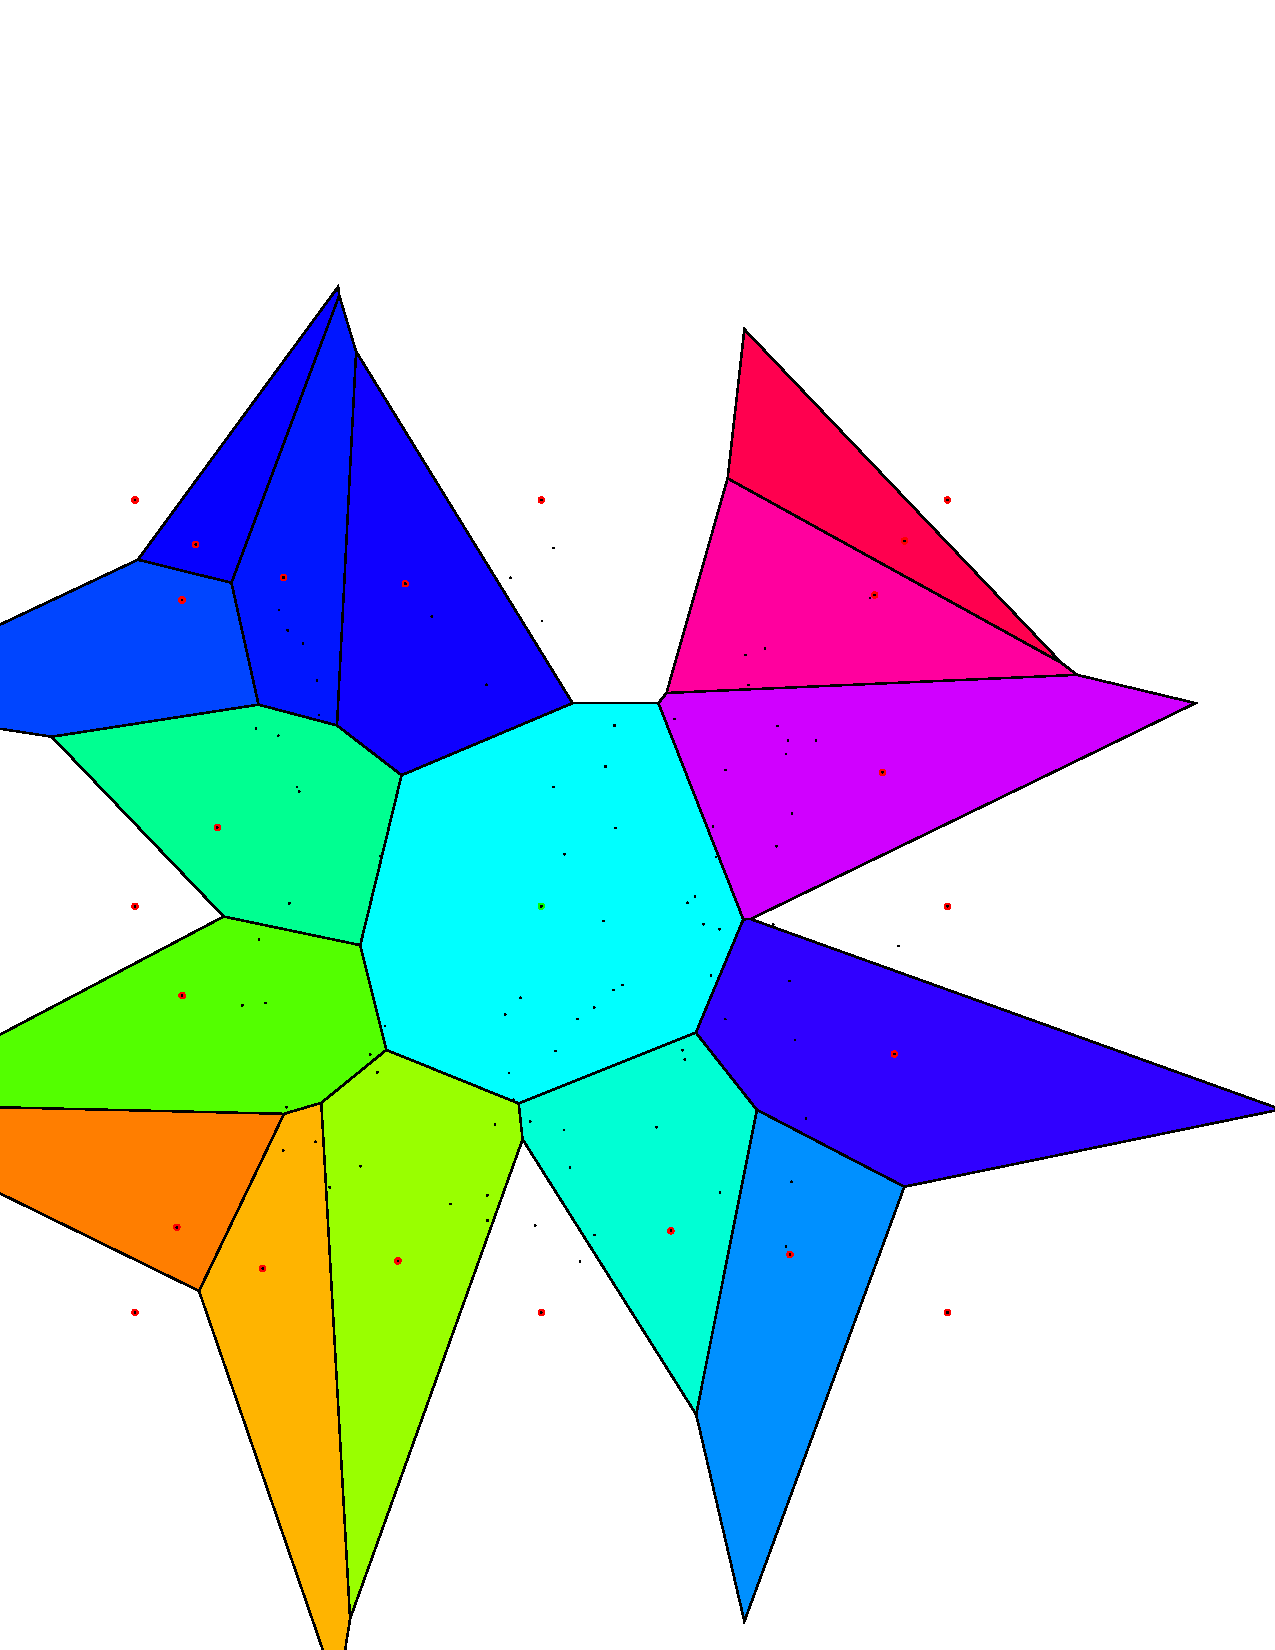
\includegraphics[trim={0 0 0 4cm},clip, width=0.45\textwidth]{../viz/100/voro0.pdf}}
   \subfloat {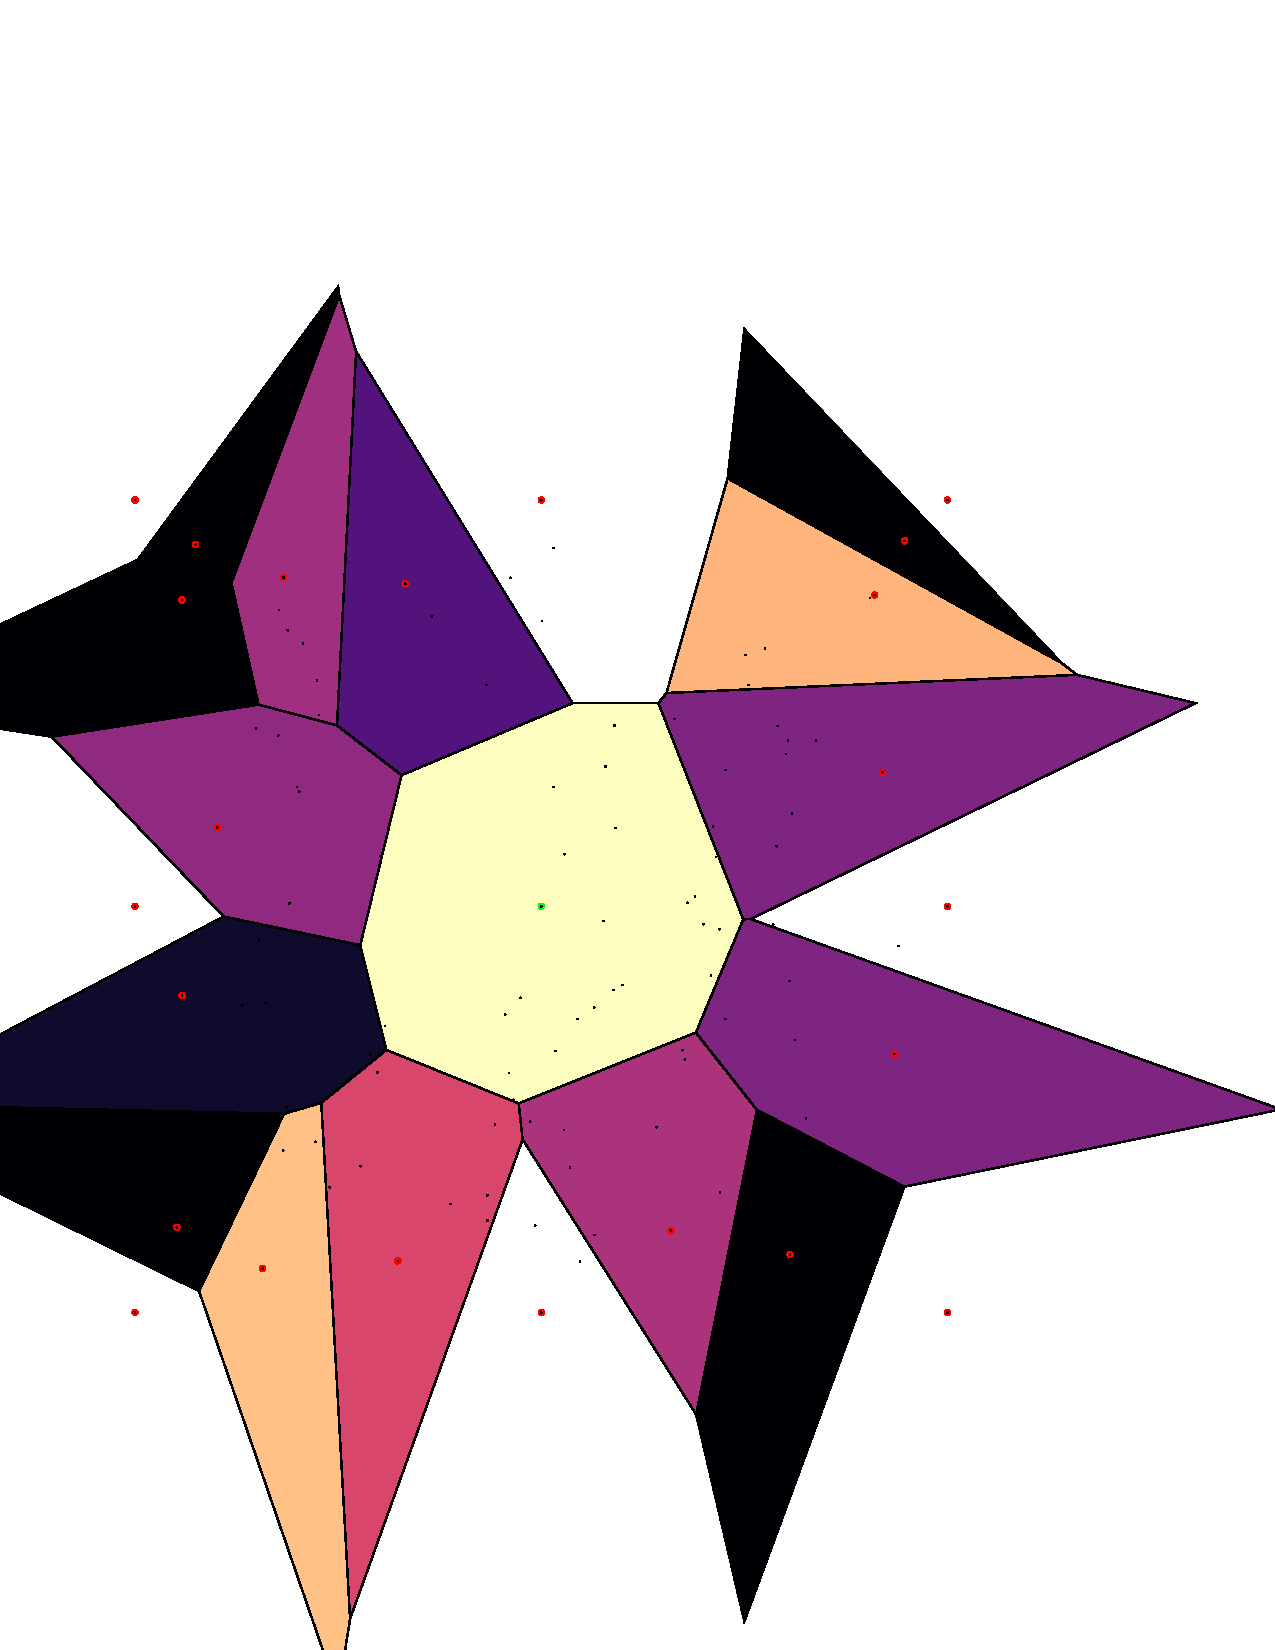
\includegraphics[trim={0 0 0 4cm},clip, width=0.45\textwidth]{../viz/100/voro_err0.pdf}}
   
   \subfloat {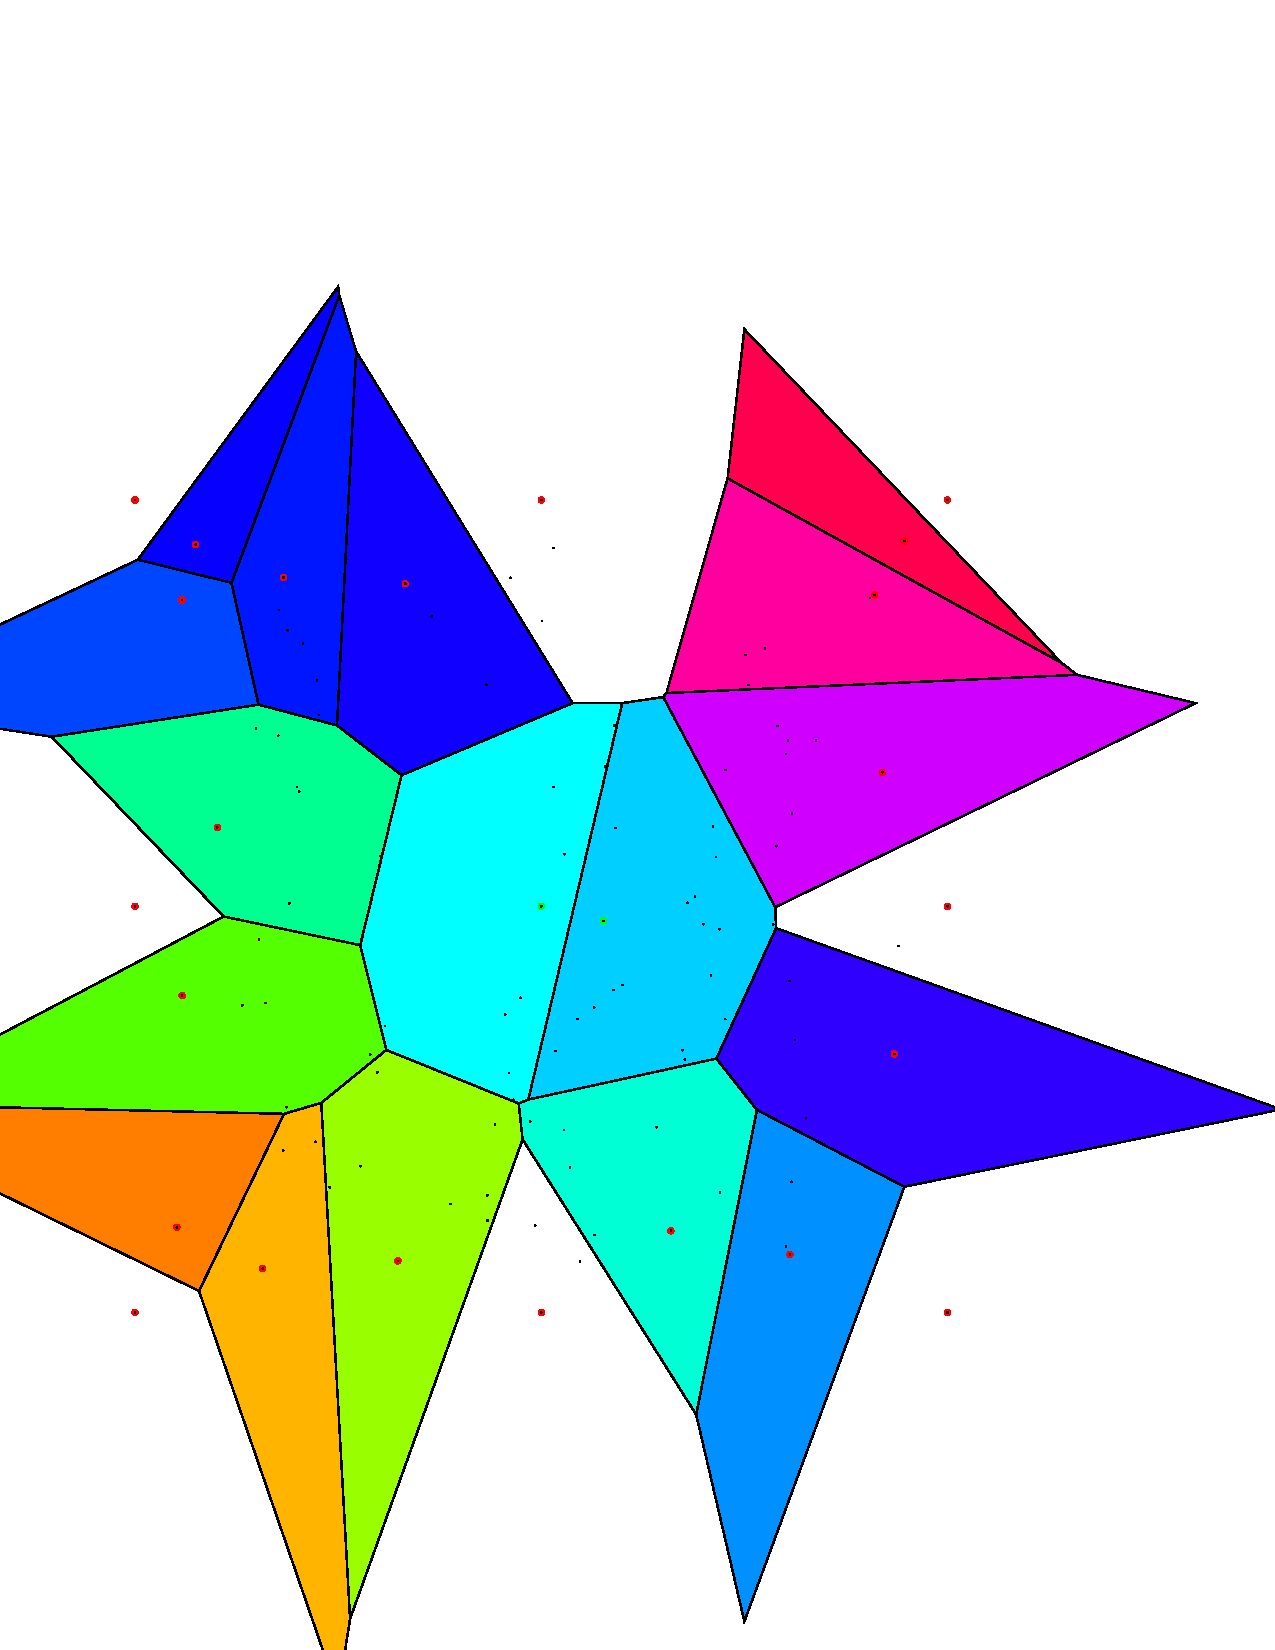
\includegraphics[trim={0 0 0 4cm},clip, width=0.45\textwidth]{../viz/100/voro1.pdf}}
   \subfloat {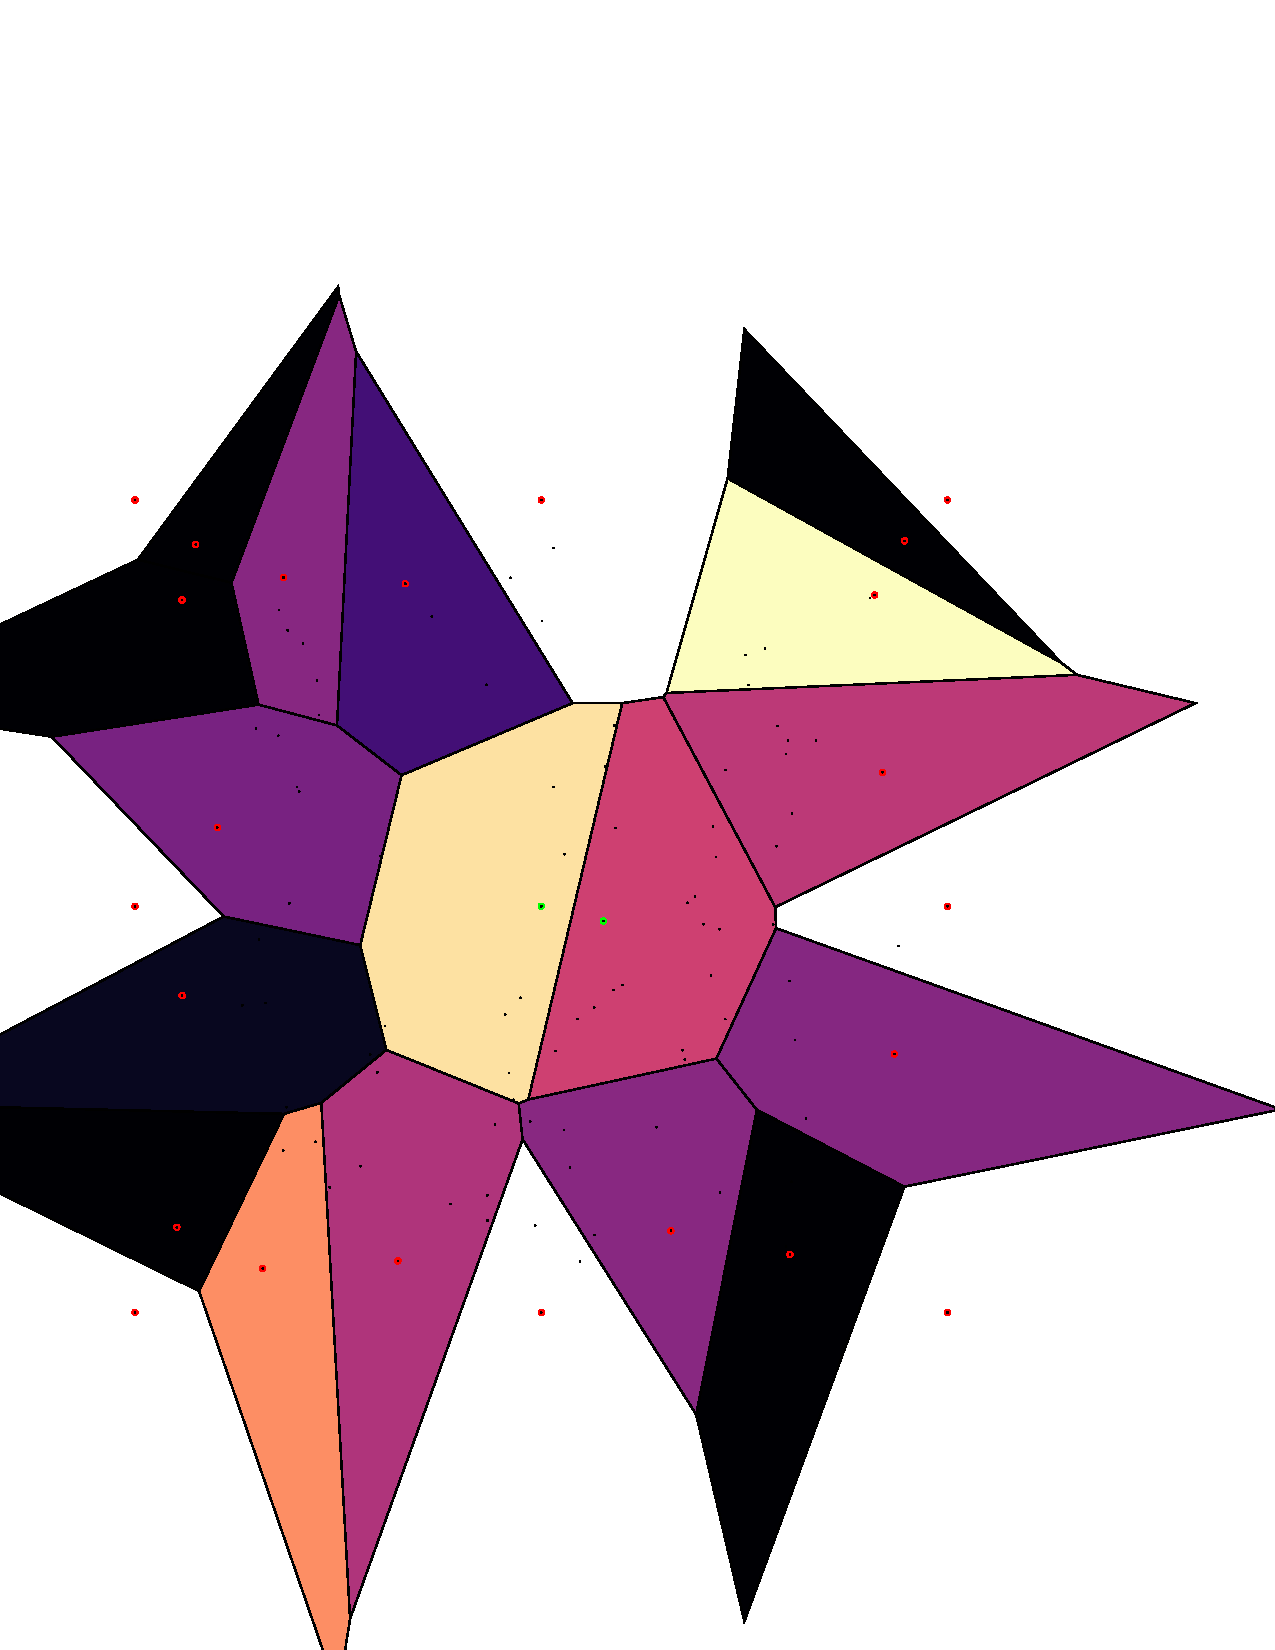
\includegraphics[trim={0 0 0 4cm},clip, width=0.45\textwidth]{../viz/100/voro_err1.pdf}}
\end{figure}
%======================================================

\newpage
\begin{figure}[!tbh]
\centering           
   \subfloat {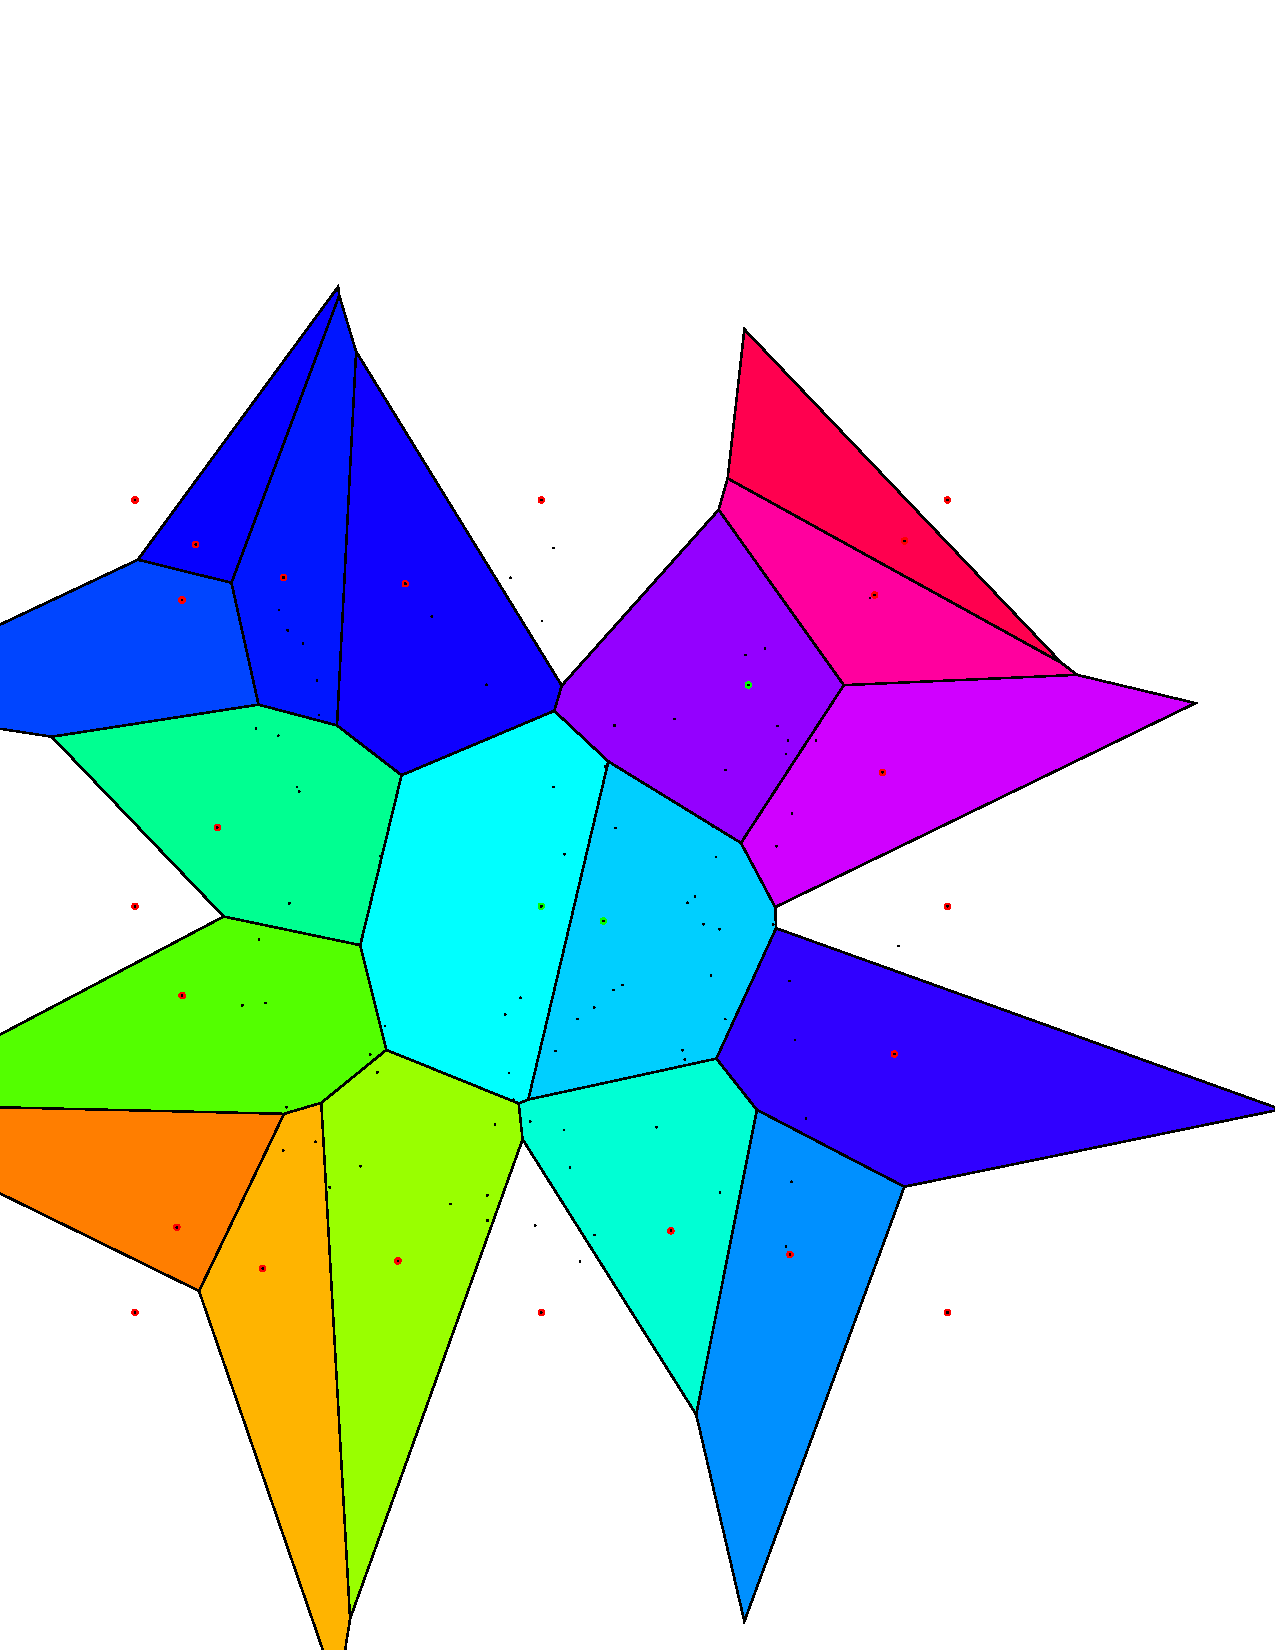
\includegraphics[trim={0 0 0 4cm},clip, width=0.45\textwidth]{../viz/100/voro2.pdf}}
   \subfloat {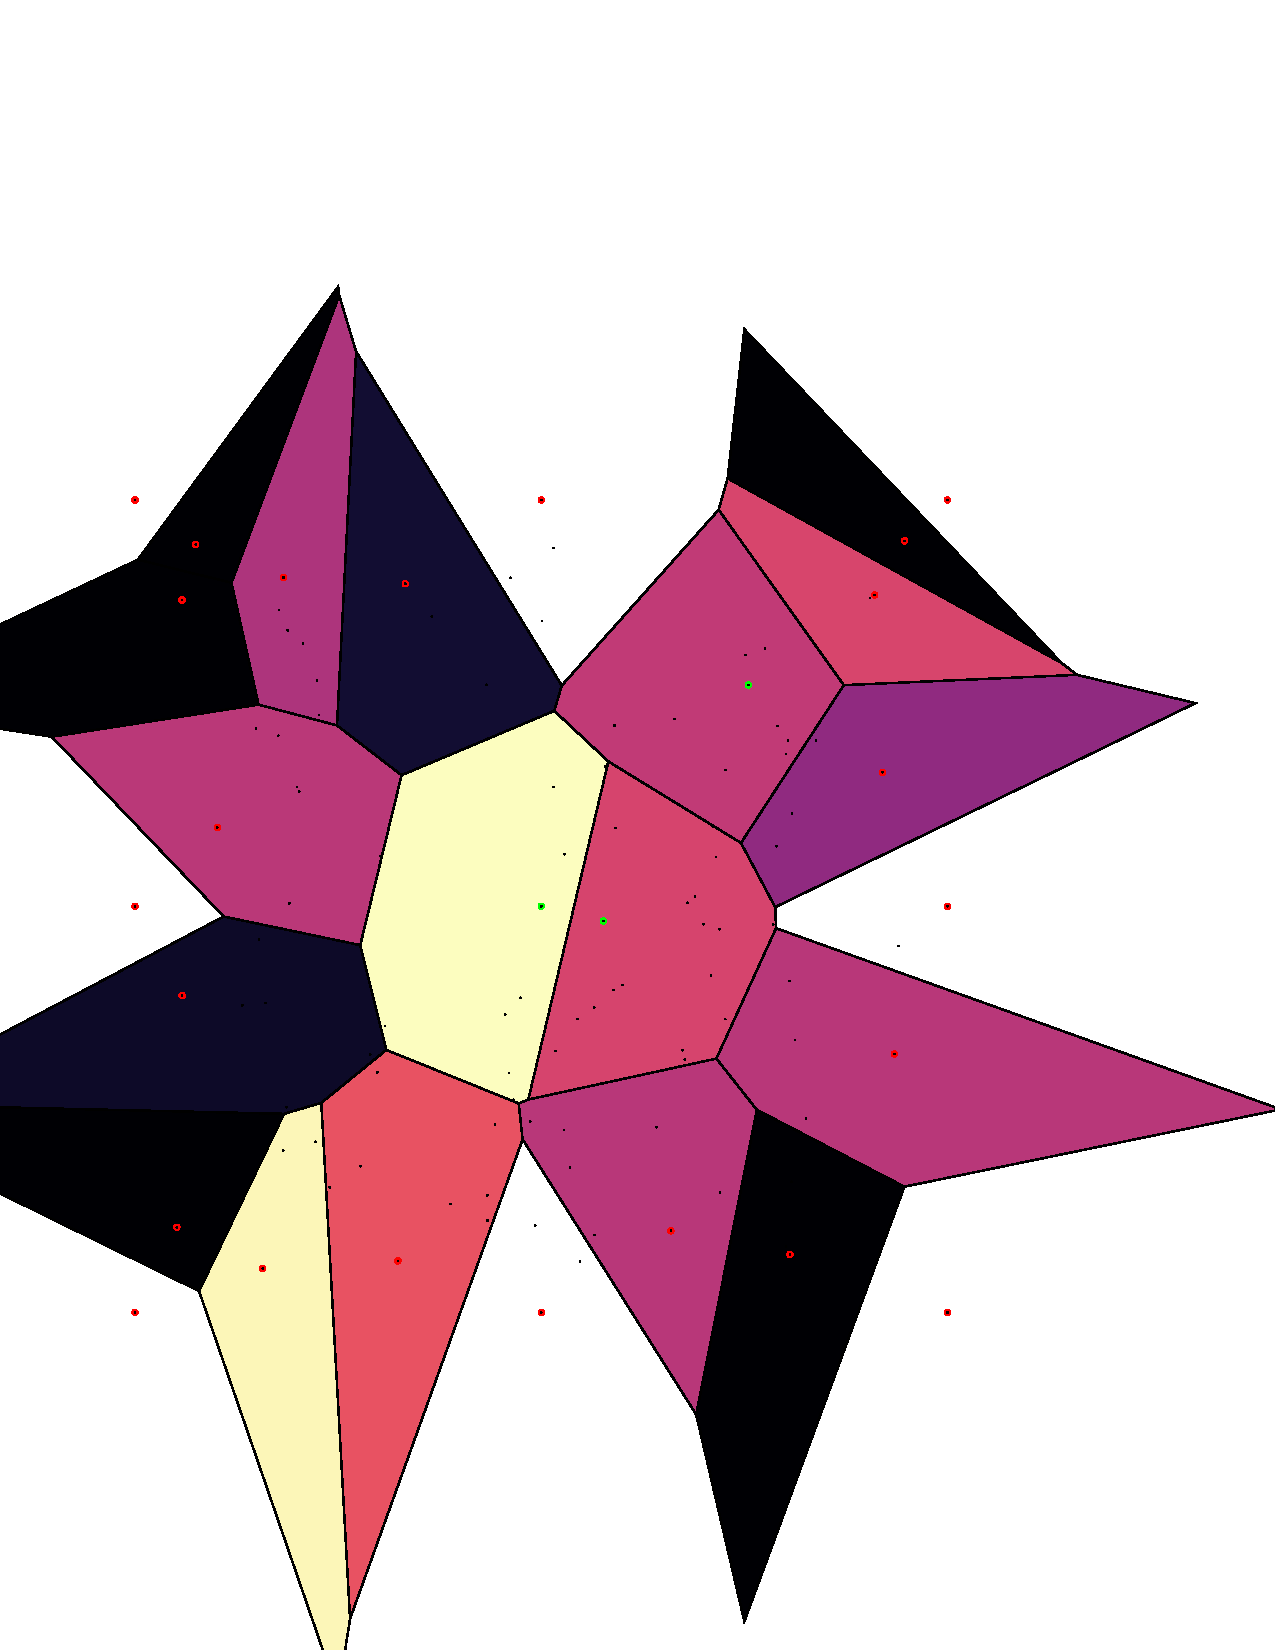
\includegraphics[trim={0 0 0 4cm},clip, width=0.45\textwidth]{../viz/100/voro_err2.pdf}}
   
   \subfloat {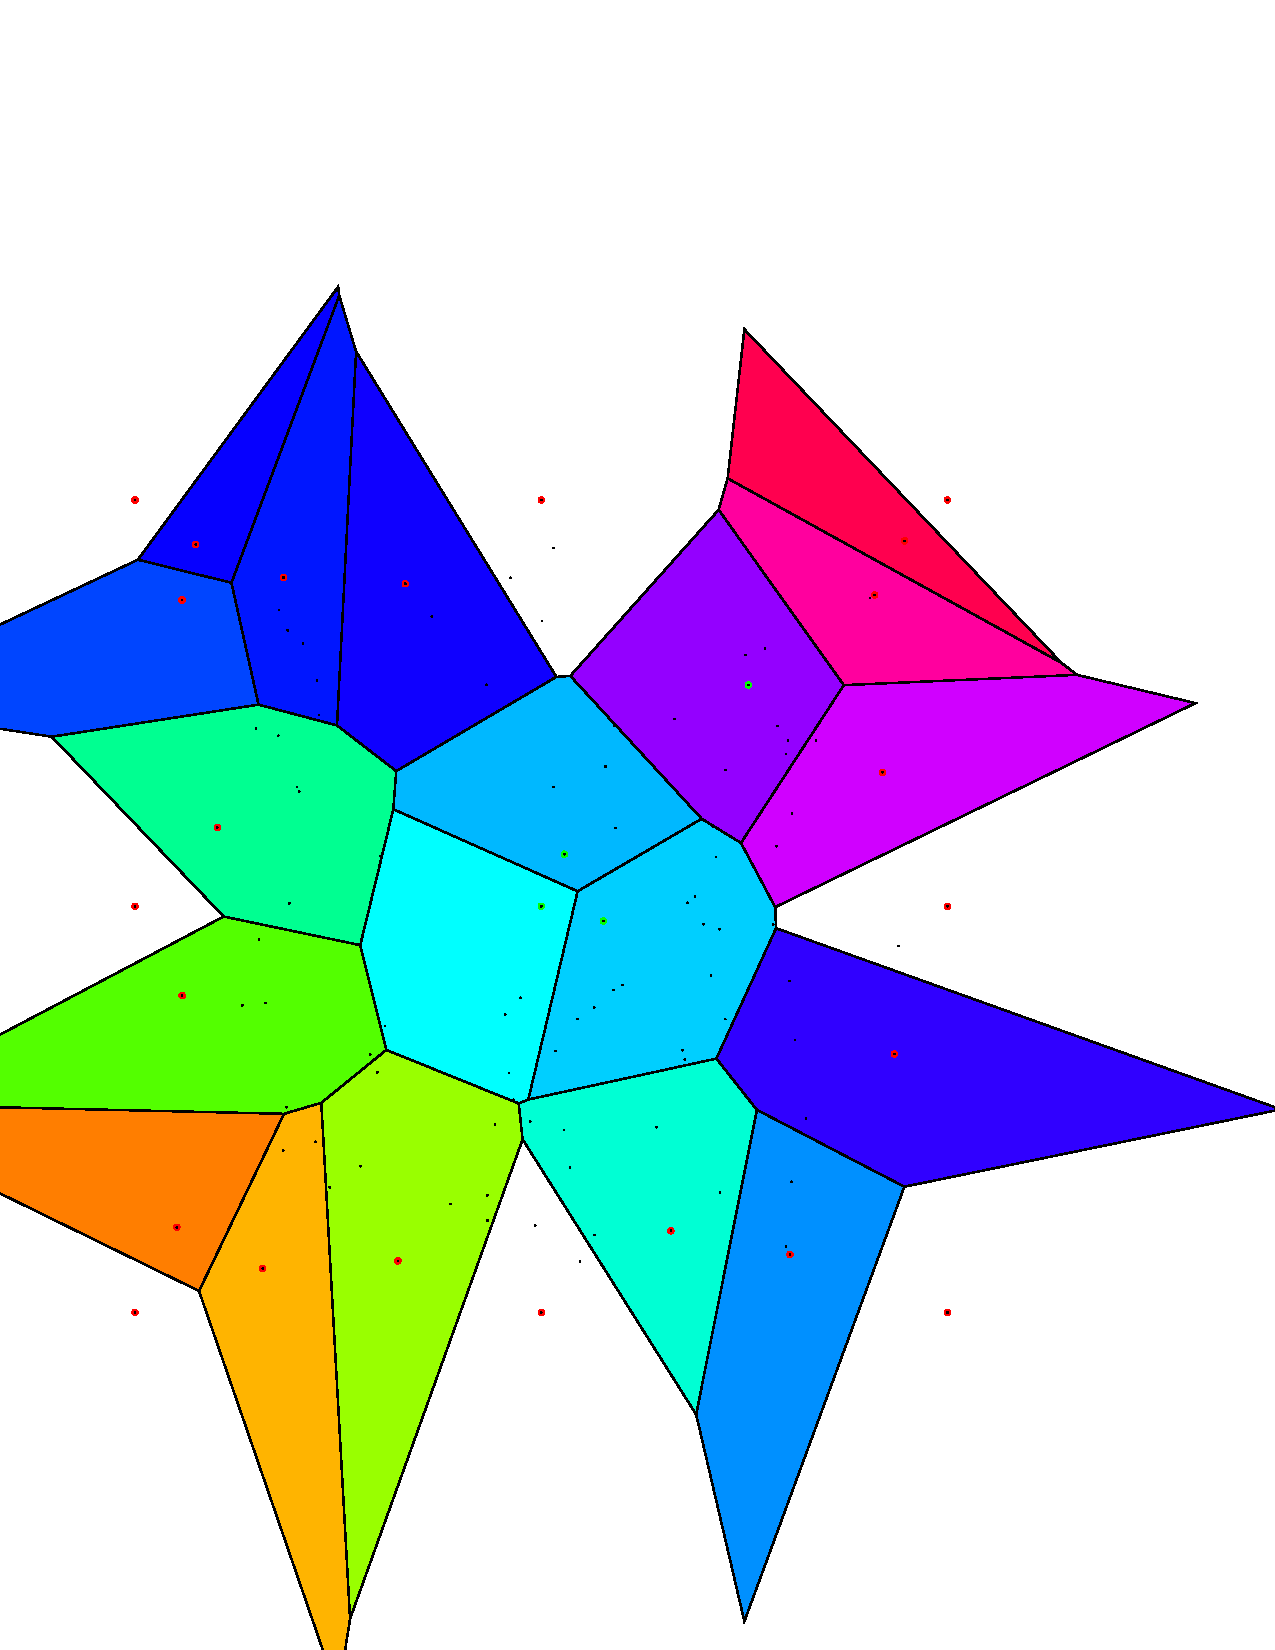
\includegraphics[trim={0 0 0 4cm},clip, width=0.45\textwidth]{../viz/100/voro3.pdf}}
   \subfloat {
\includegraphics[trim={0 0 0 4cm},clip, width=0.45\textwidth]{../viz/100/voro_err3.pdf}}
\end{figure}
%======================================================

\newpage
\begin{figure}[!tbh]
\centering           
   \subfloat {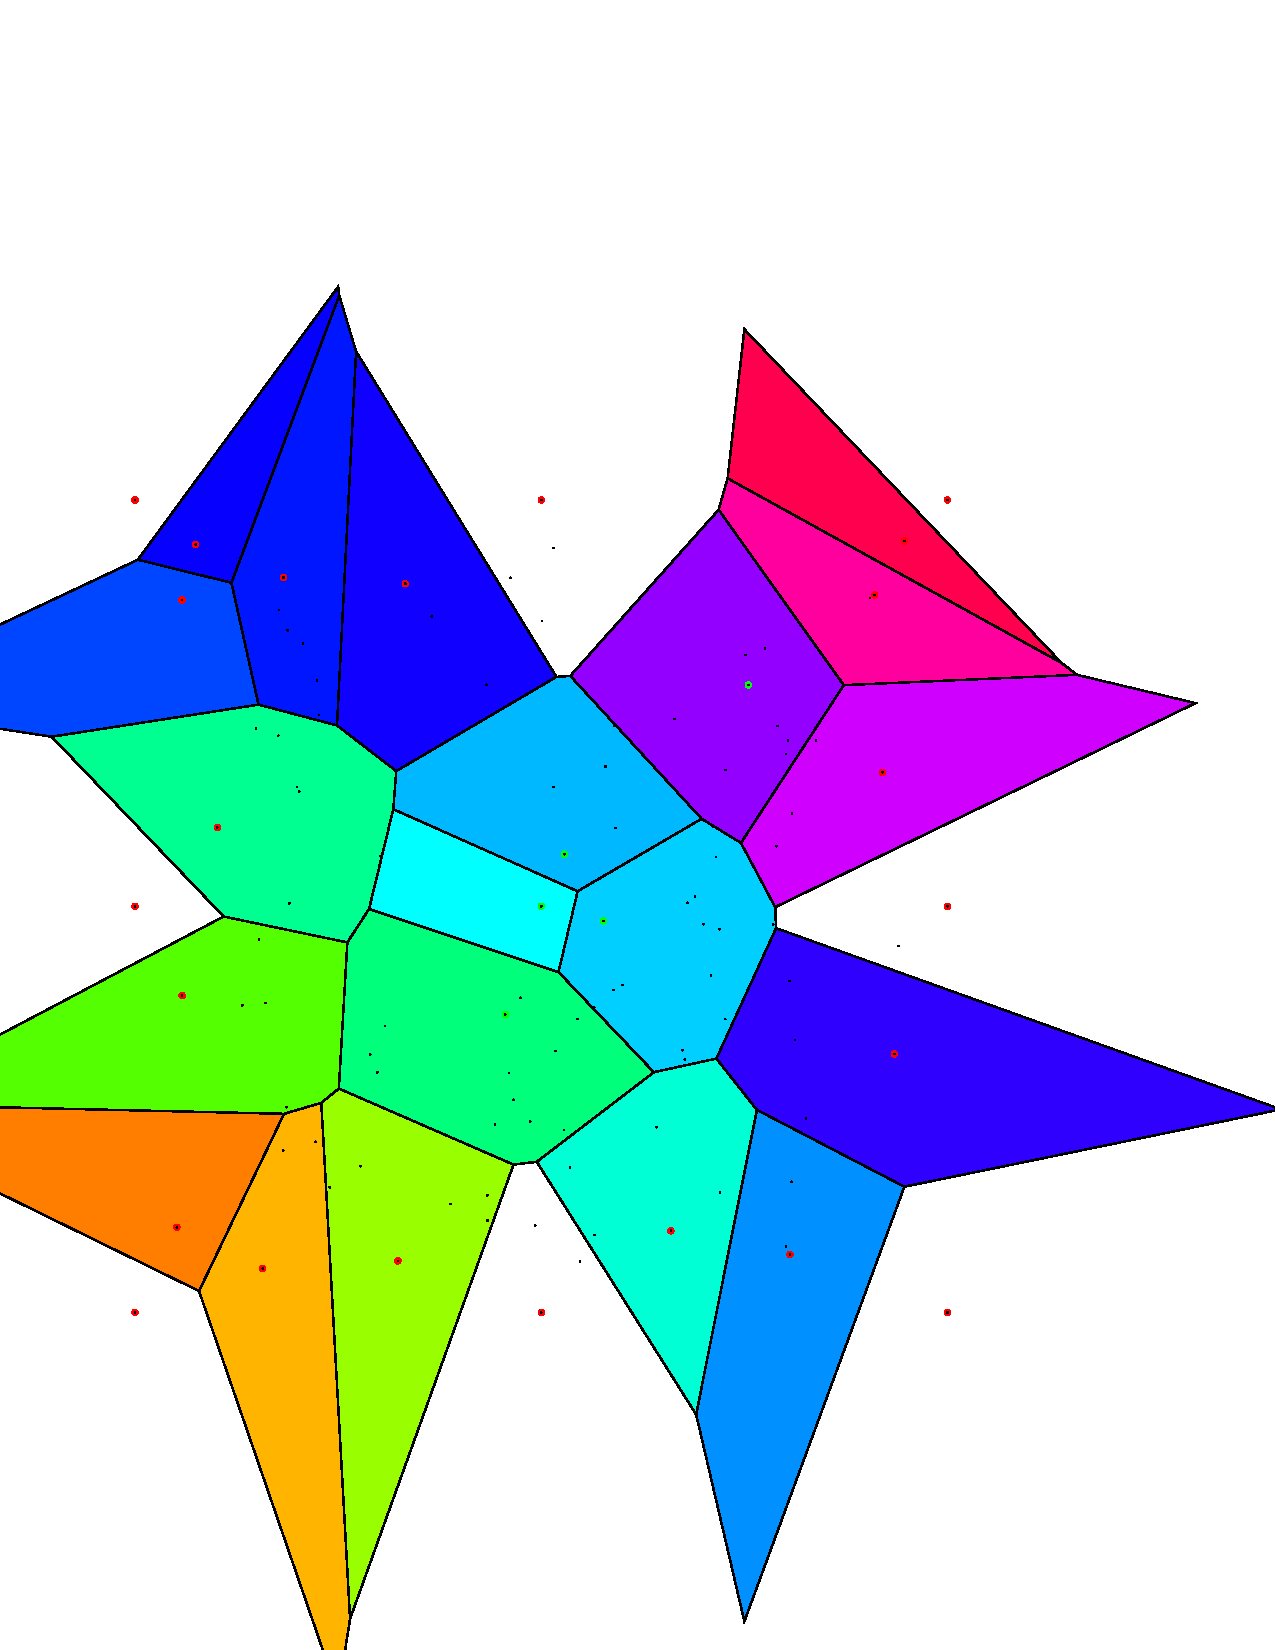
\includegraphics[trim={0 0 0 4cm},clip, width=0.45\textwidth]{../viz/100/voro4.pdf}}
   \subfloat {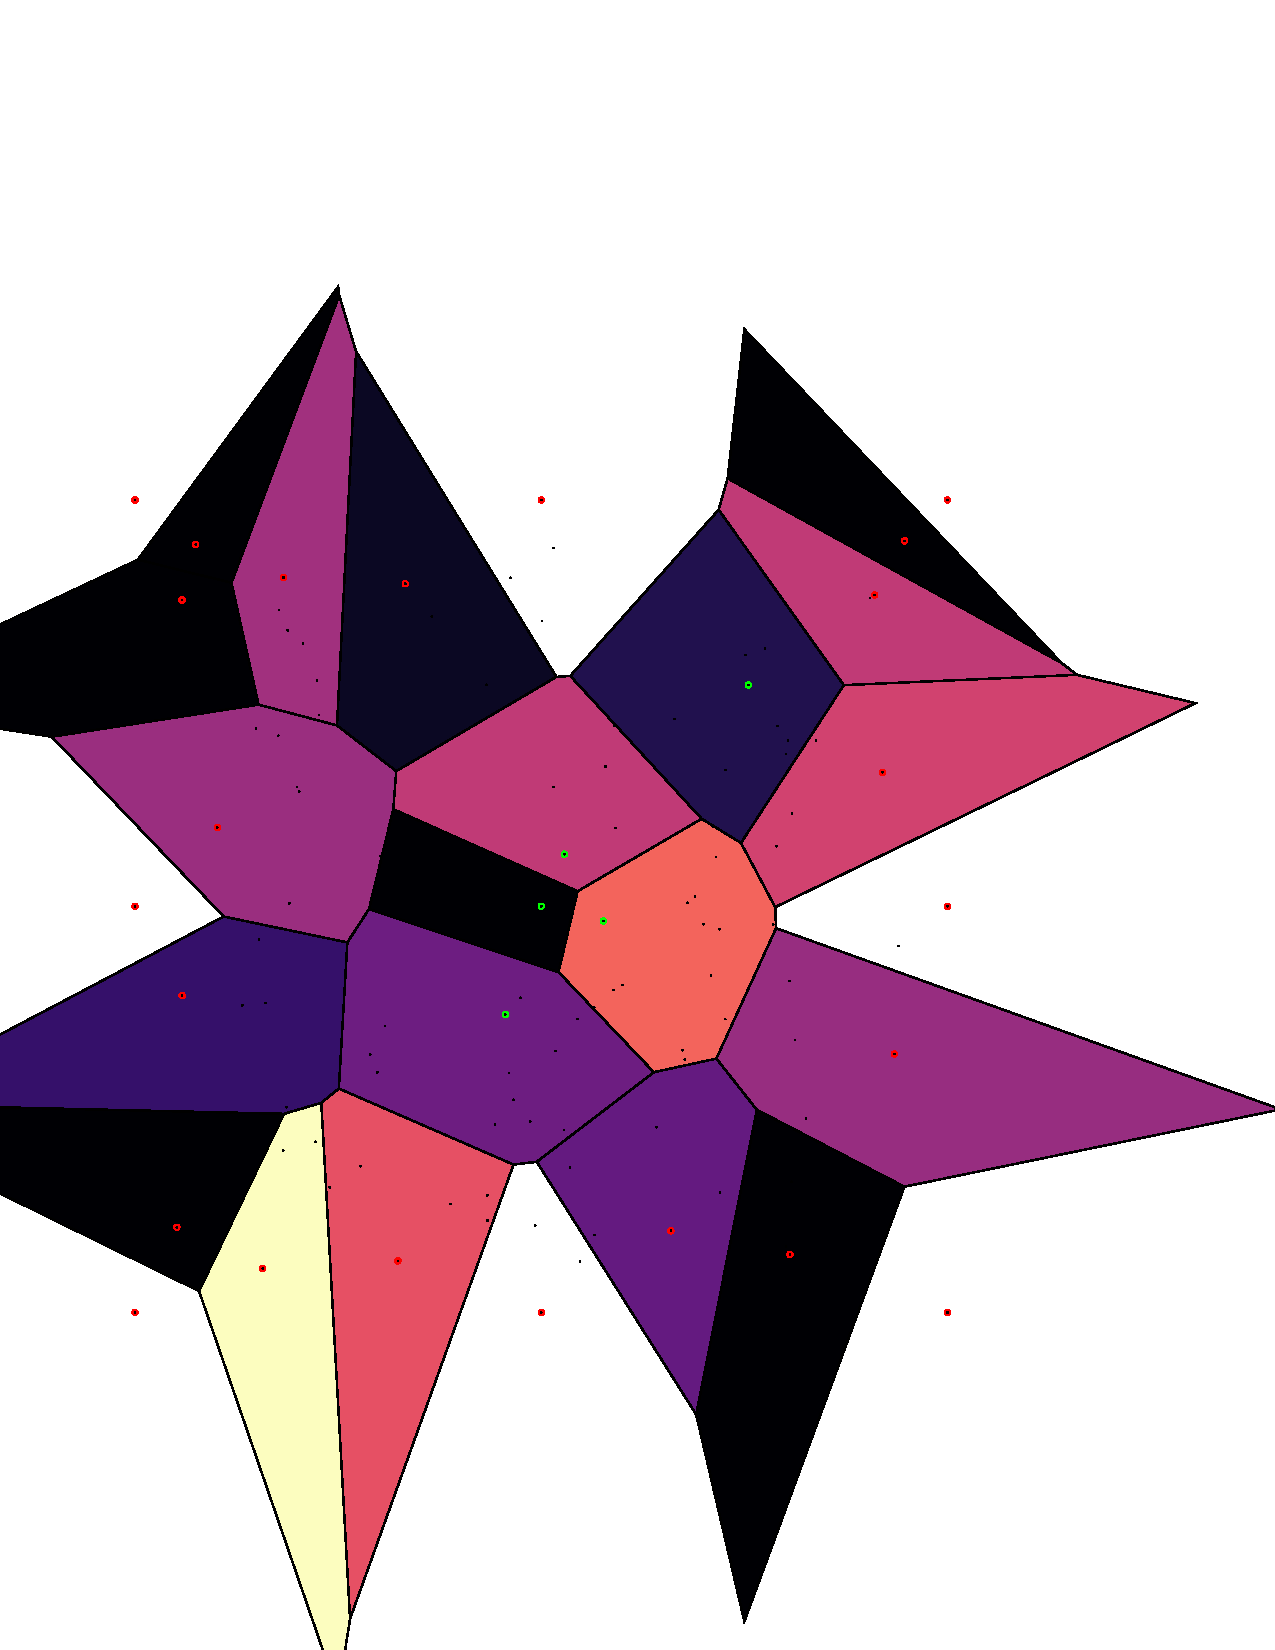
\includegraphics[trim={0 0 0 4cm},clip, width=0.45\textwidth]{../viz/100/voro_err4.pdf}}
   
   \subfloat {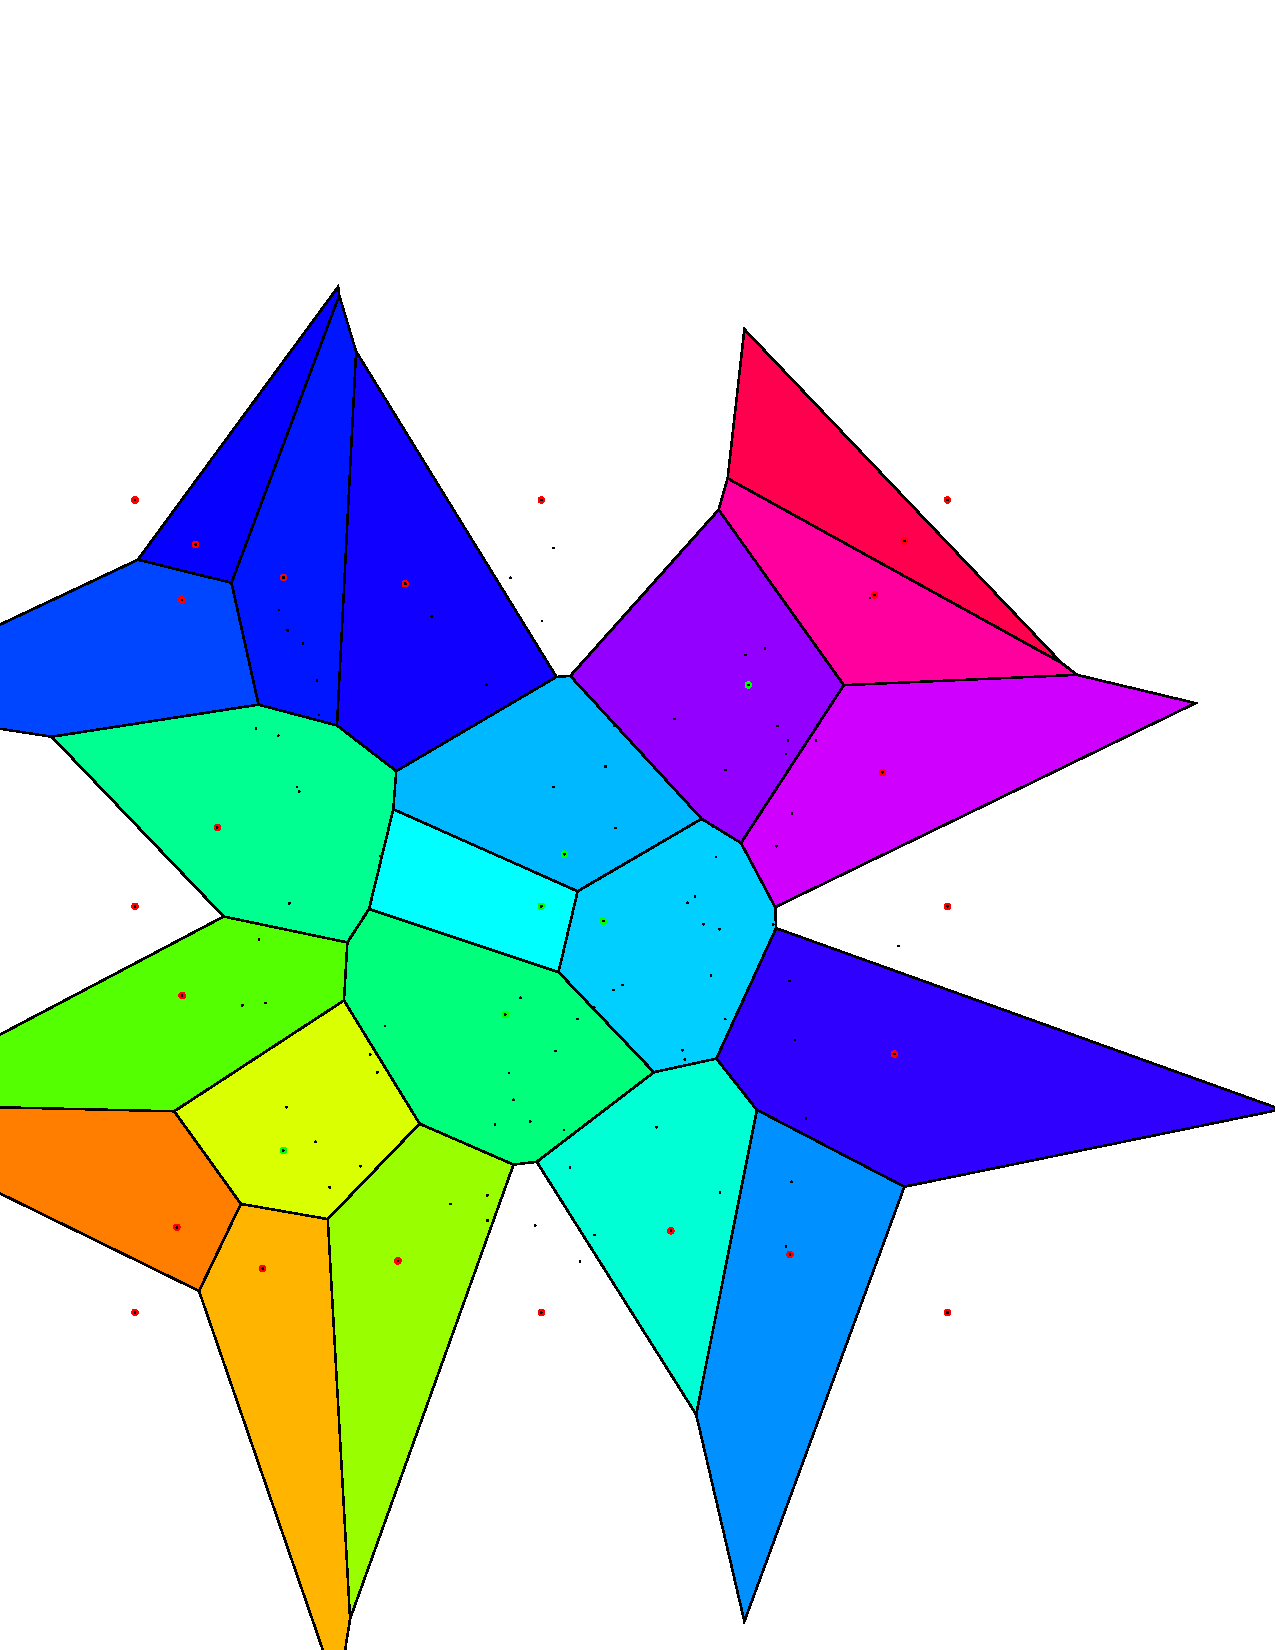
\includegraphics[trim={0 0 0 4cm},clip, width=0.45\textwidth]{../viz/100/voro5.pdf}}
   \subfloat {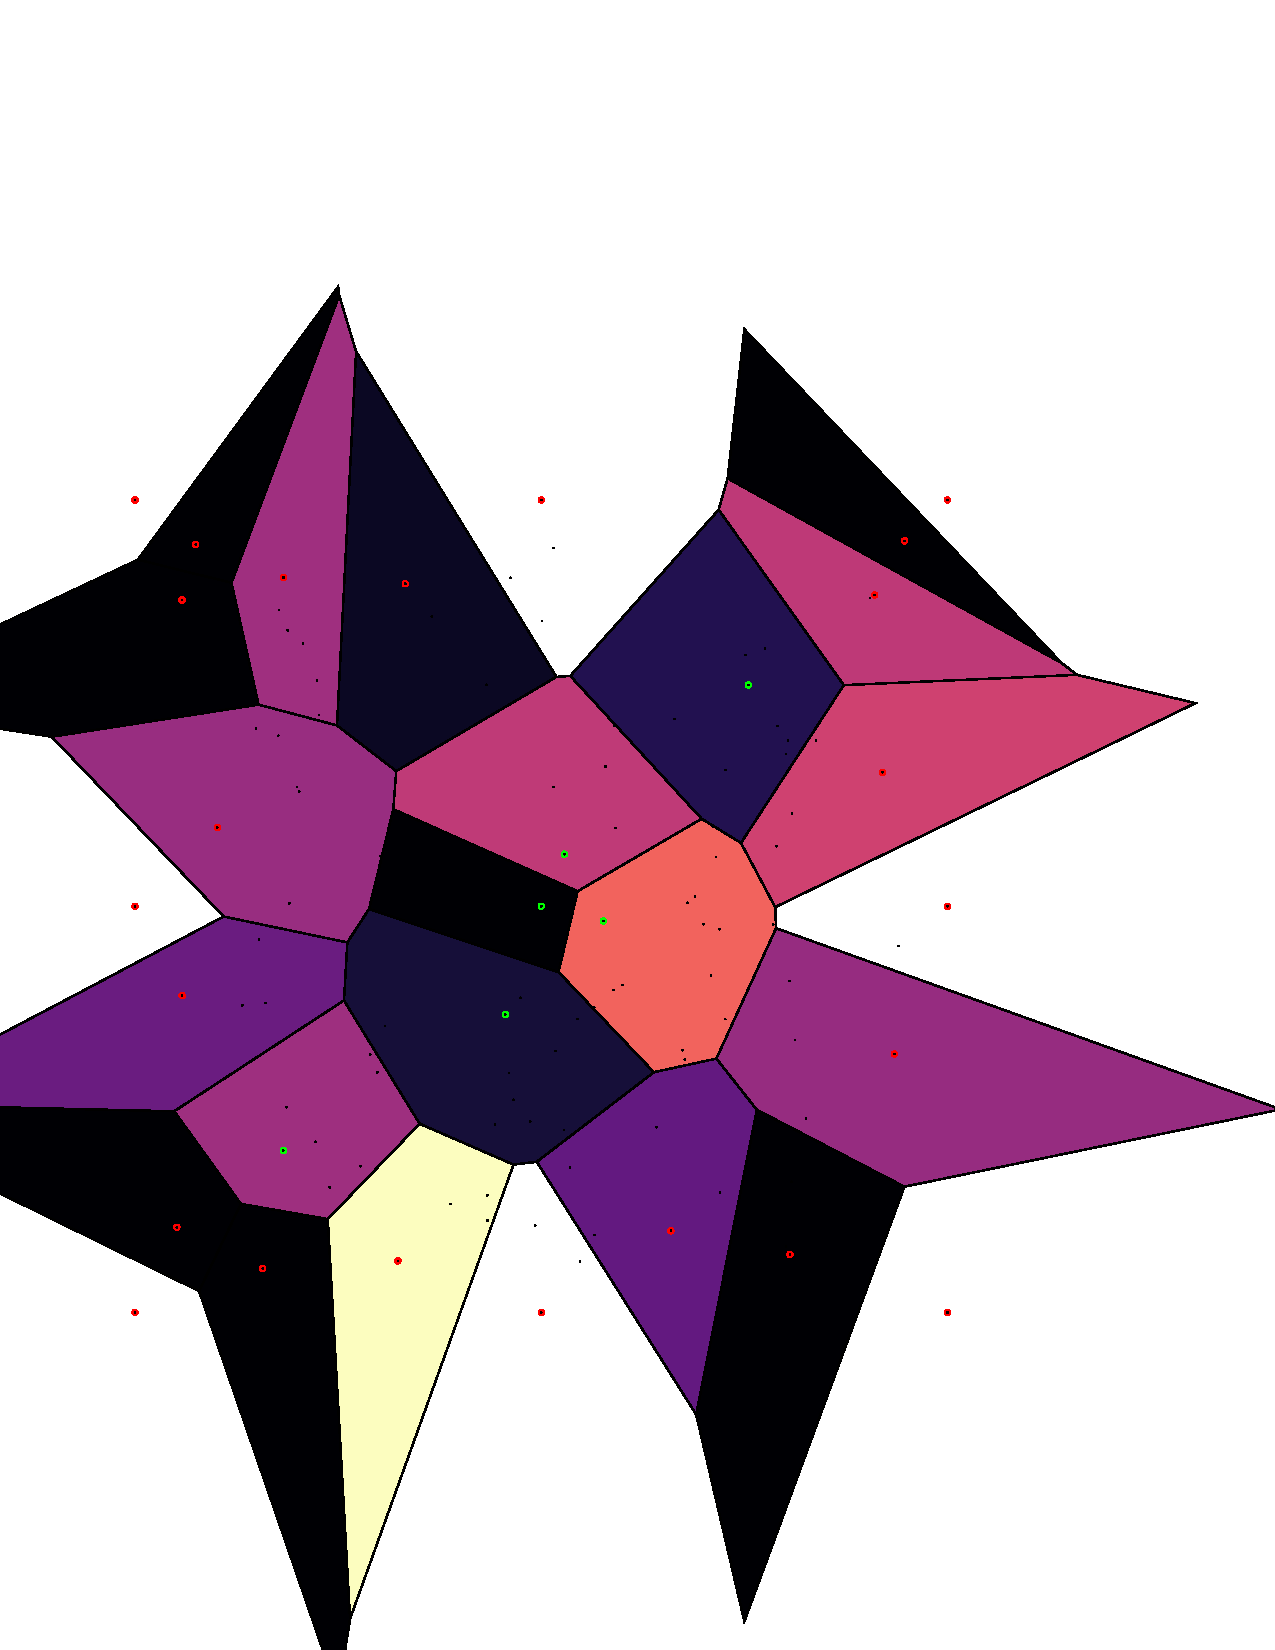
\includegraphics[trim={0 0 0 4cm},clip, width=0.45\textwidth]{../viz/100/voro_err5.pdf}}
\end{figure}
%======================================================

\newpage
\begin{figure}[!tbh]
\centering           
   \subfloat {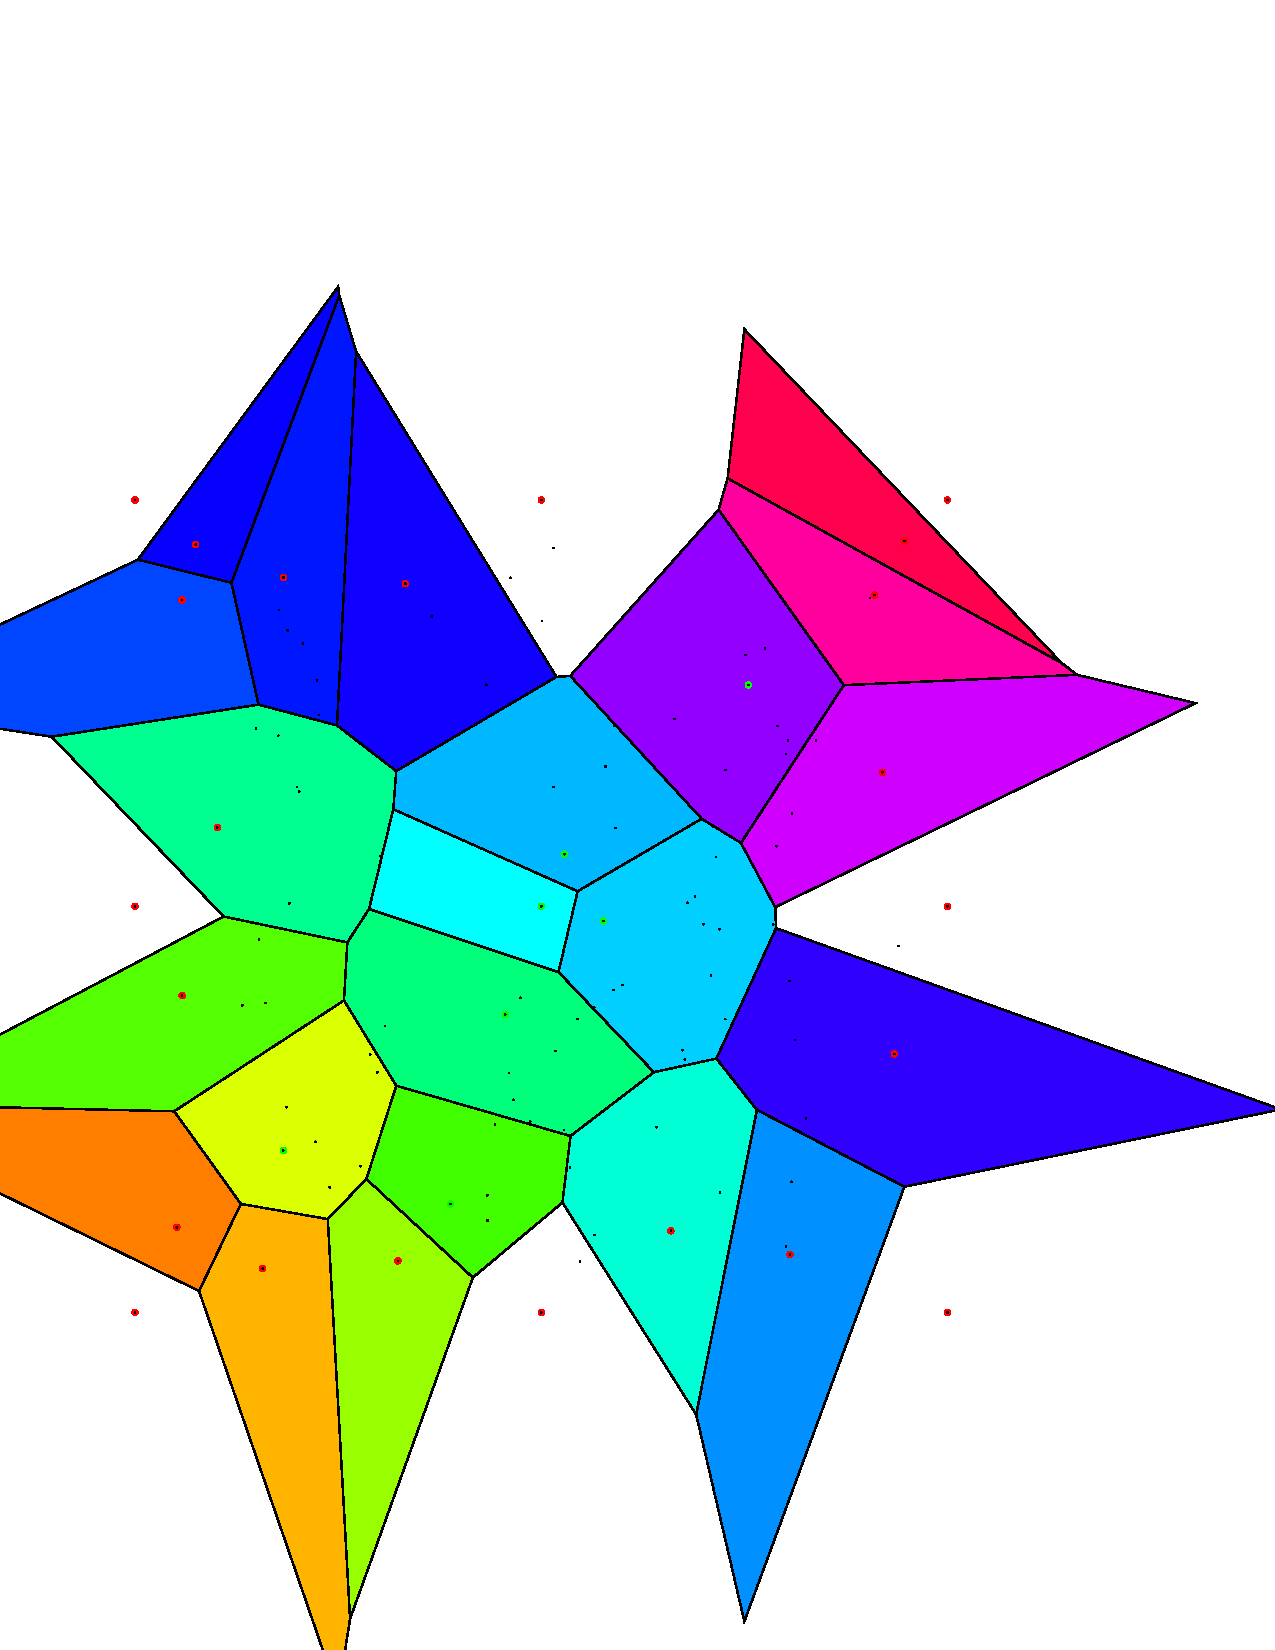
\includegraphics[trim={0 0 0 4cm},clip, width=0.45\textwidth]{../viz/100/voro6.pdf}}
   \subfloat {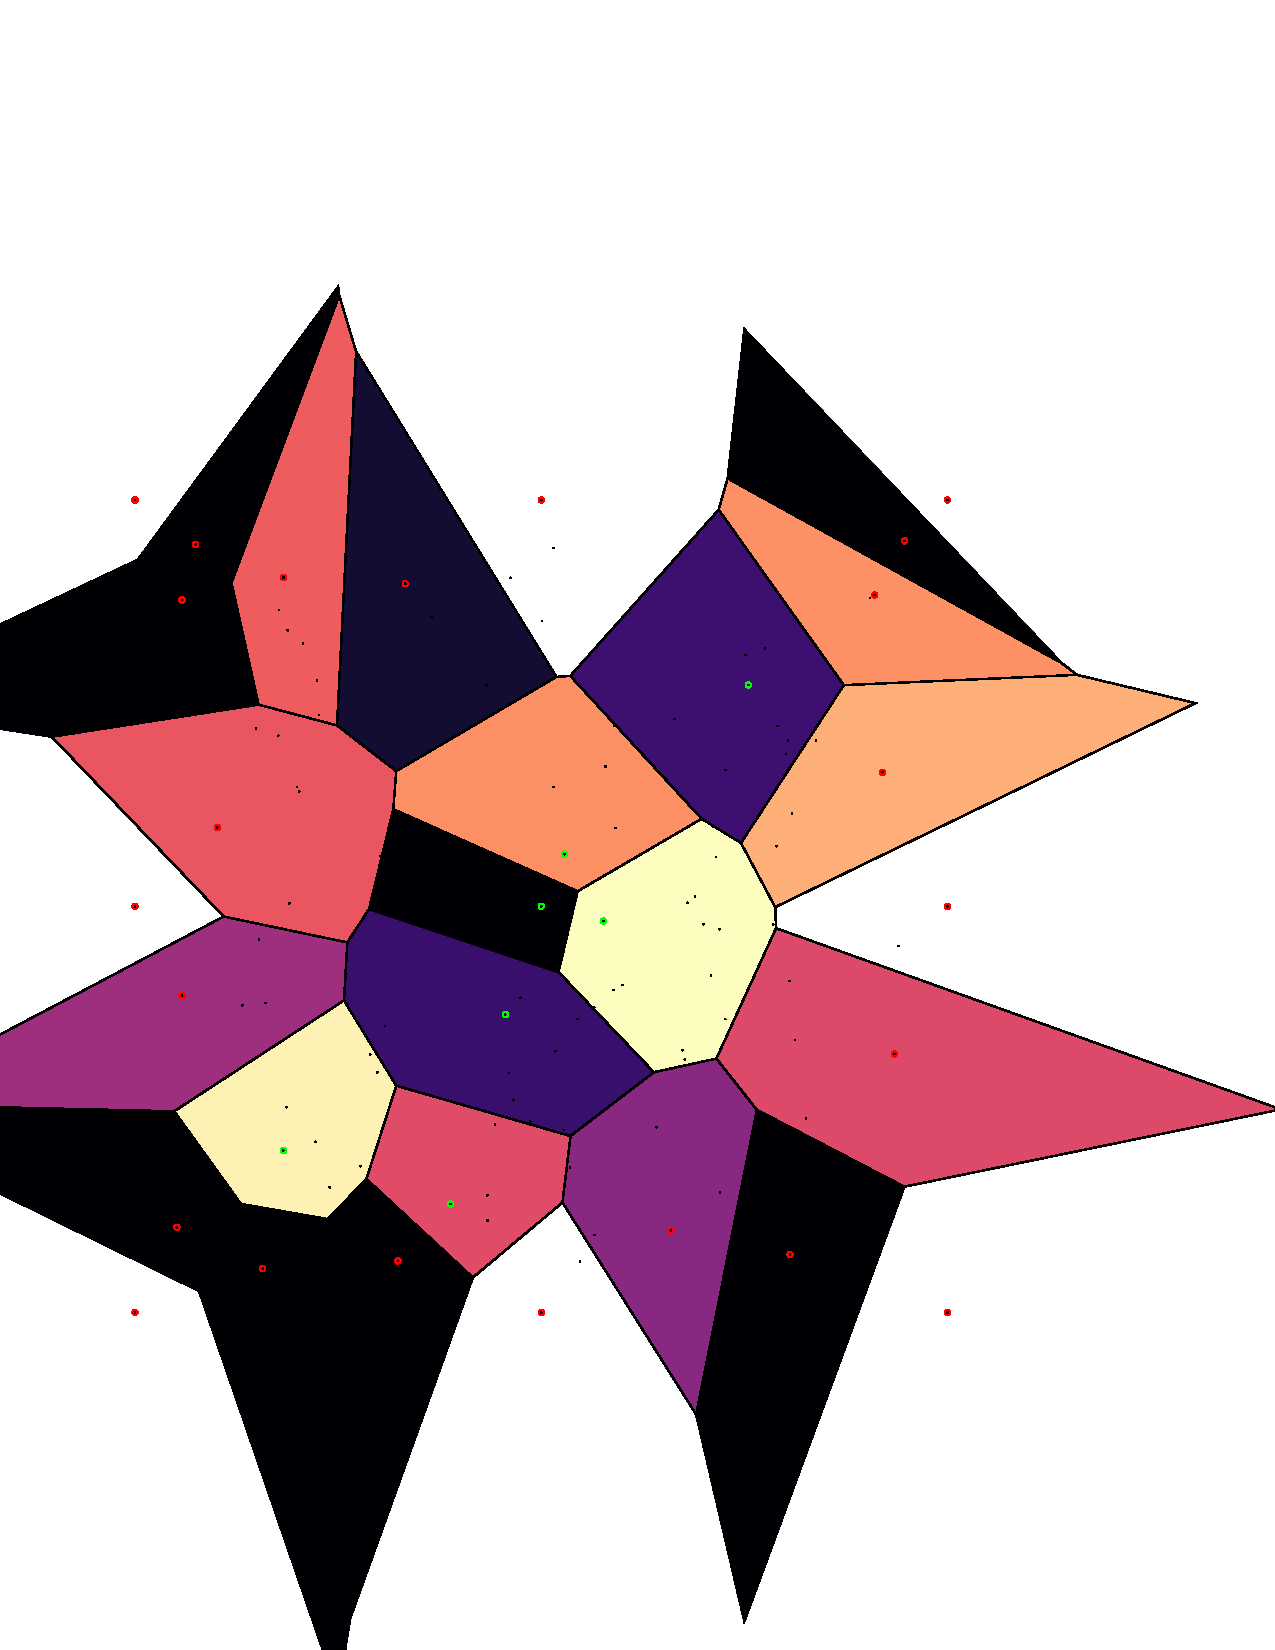
\includegraphics[trim={0 0 0 4cm},clip, width=0.45\textwidth]{../viz/100/voro_err6.pdf}}
   
   \subfloat {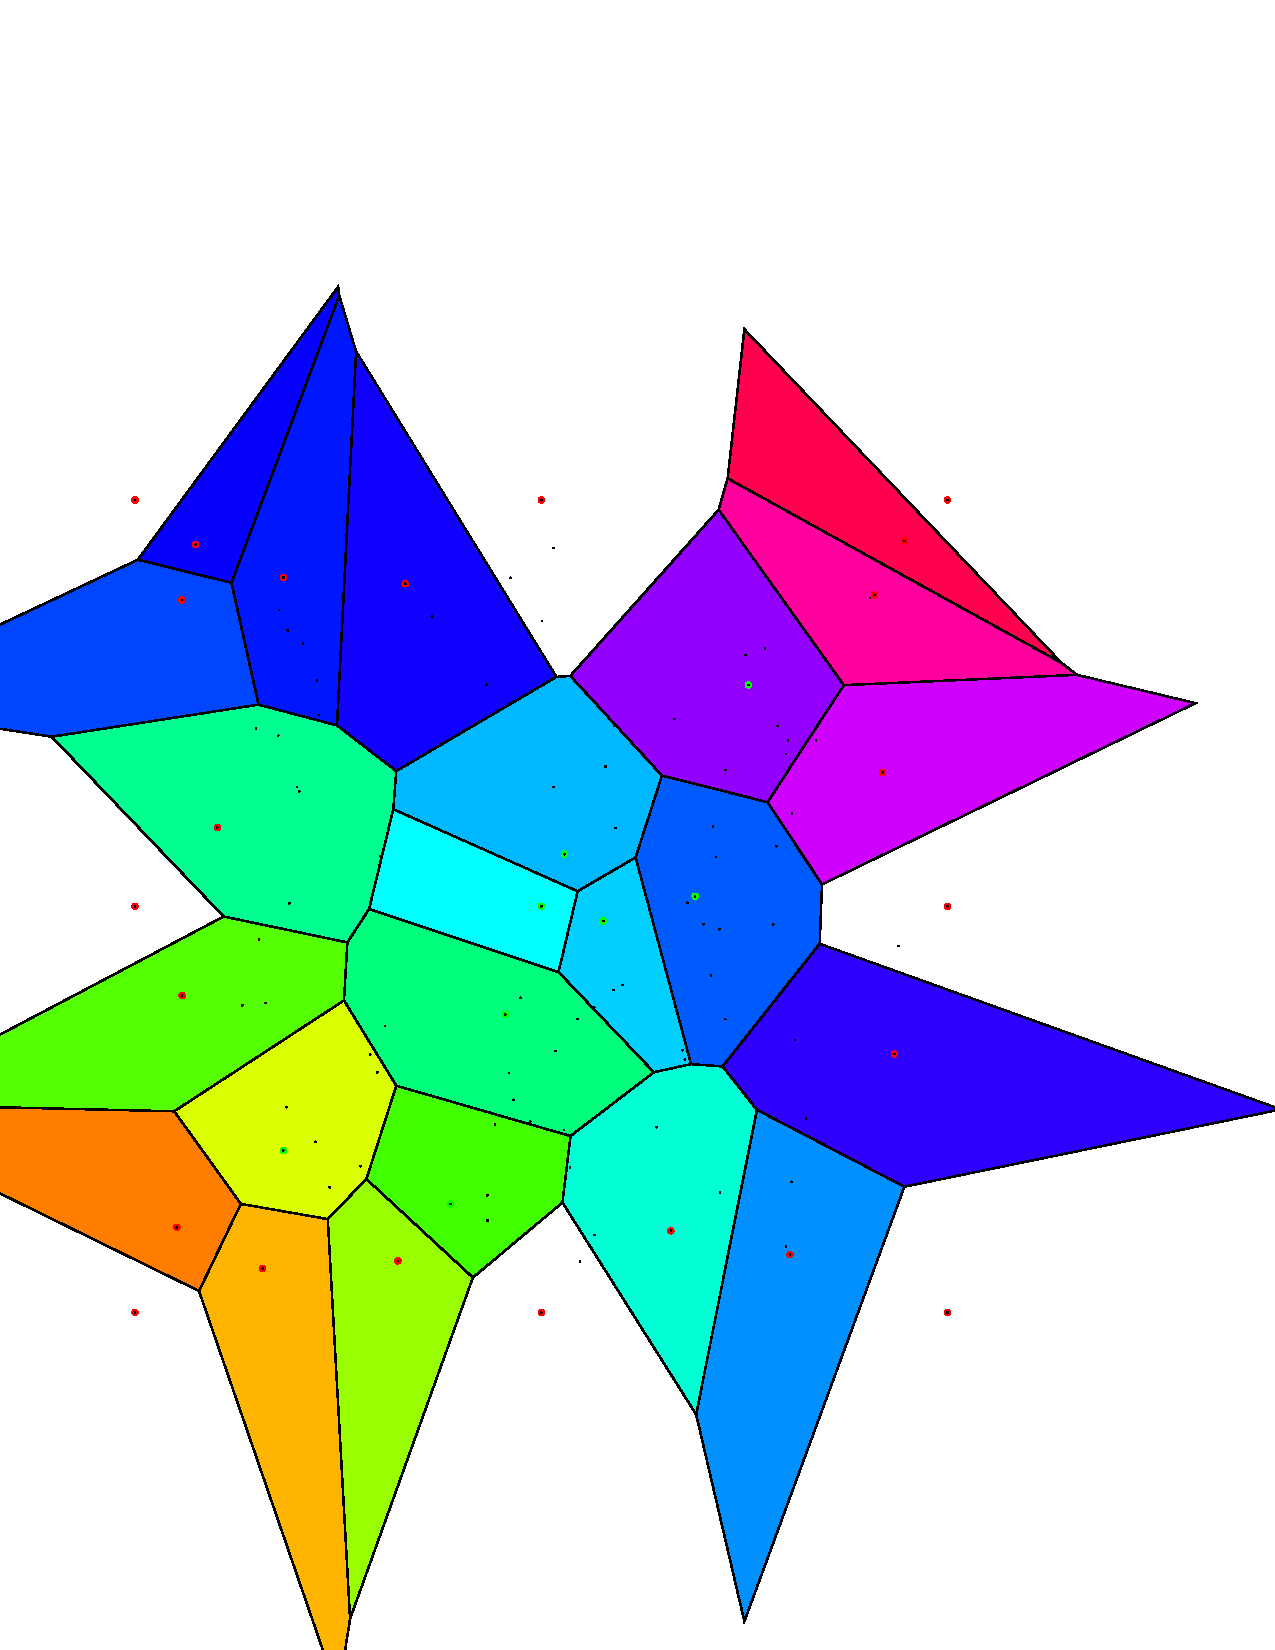
\includegraphics[trim={0 0 0 4cm},clip, width=0.45\textwidth]{../viz/100/voro7.pdf}}
   \subfloat {
\includegraphics[trim={0 0 0 4cm},clip, width=0.45\textwidth]{../viz/100/voro_err7.pdf}}
\end{figure}
%======================================================

\newpage
\begin{figure}[!tbh]
\centering           
   \subfloat {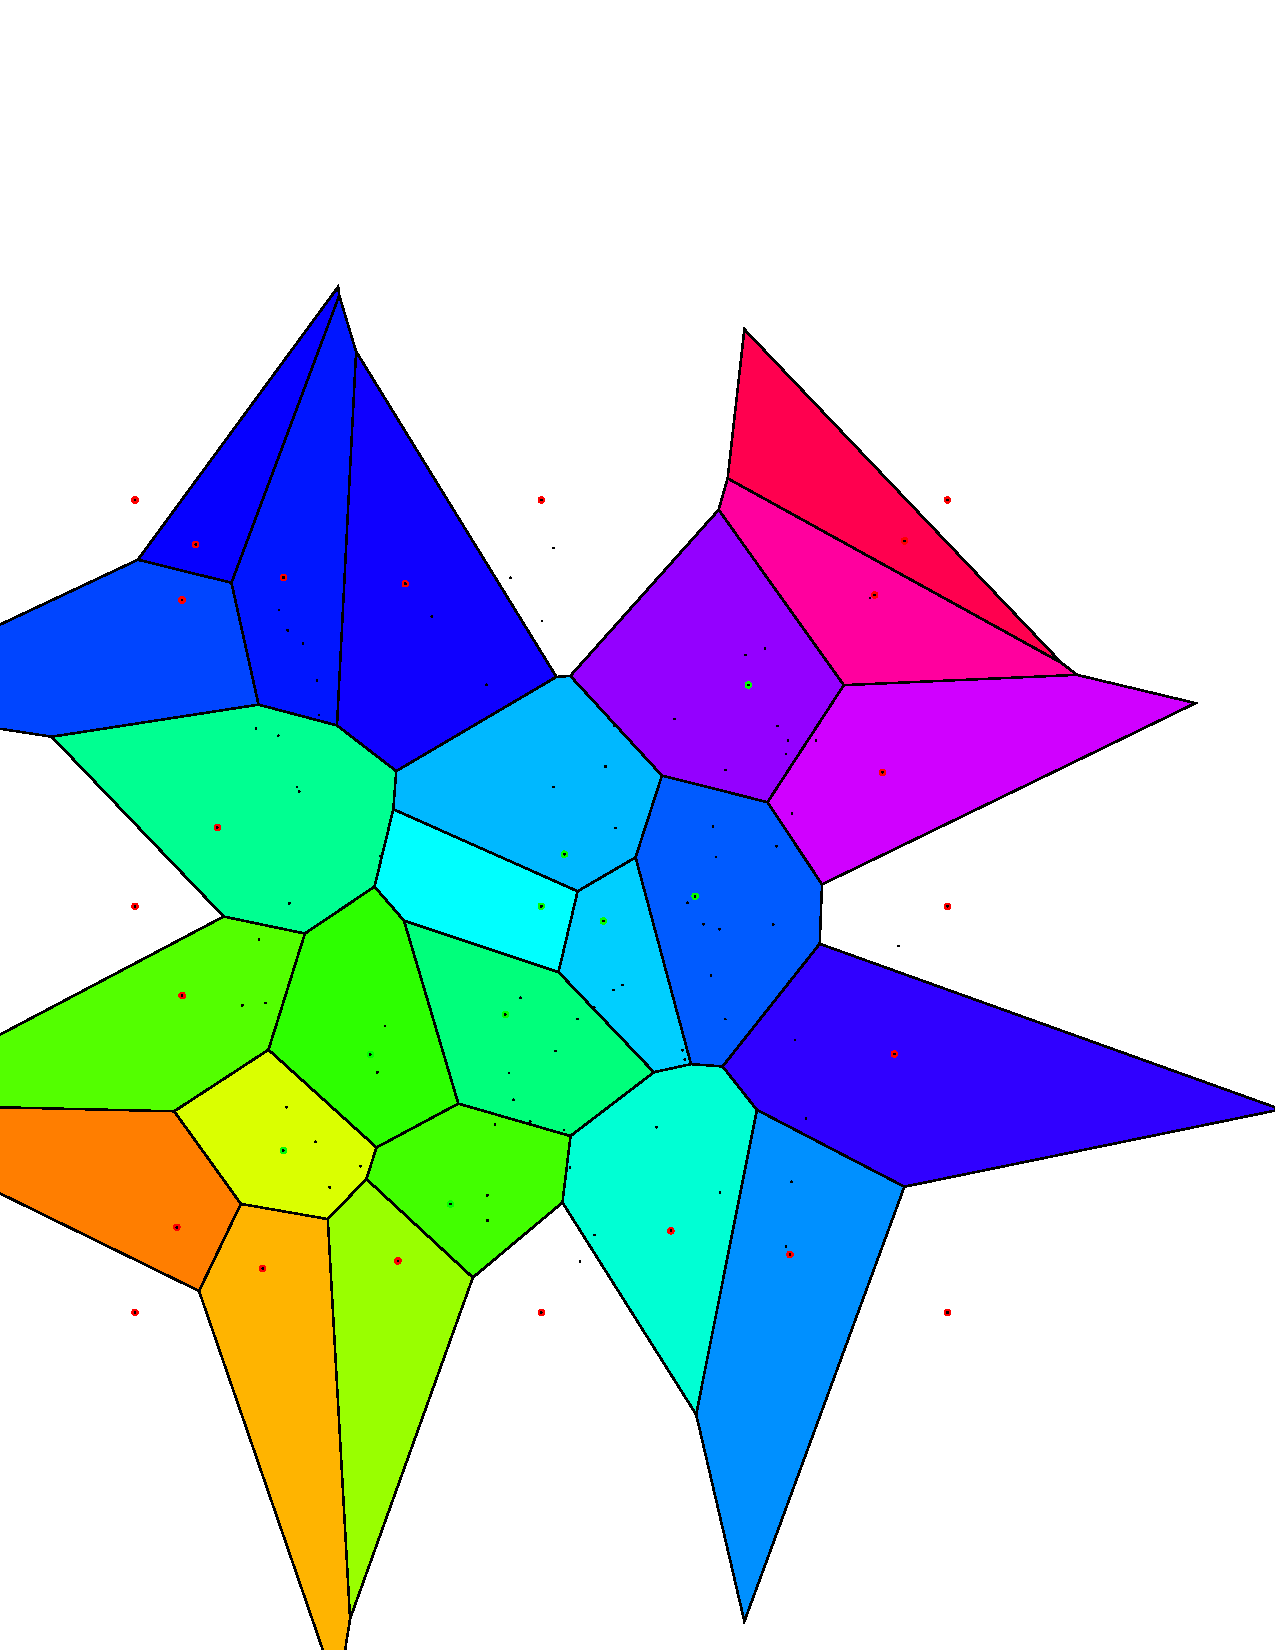
\includegraphics[trim={0 0 0 4cm},clip, width=0.45\textwidth]{../viz/100/voro8.pdf}}
   \subfloat {
\includegraphics[trim={0 0 0 4cm},clip, width=0.45\textwidth]{../viz/100/voro_err8.pdf}}
   
   \subfloat {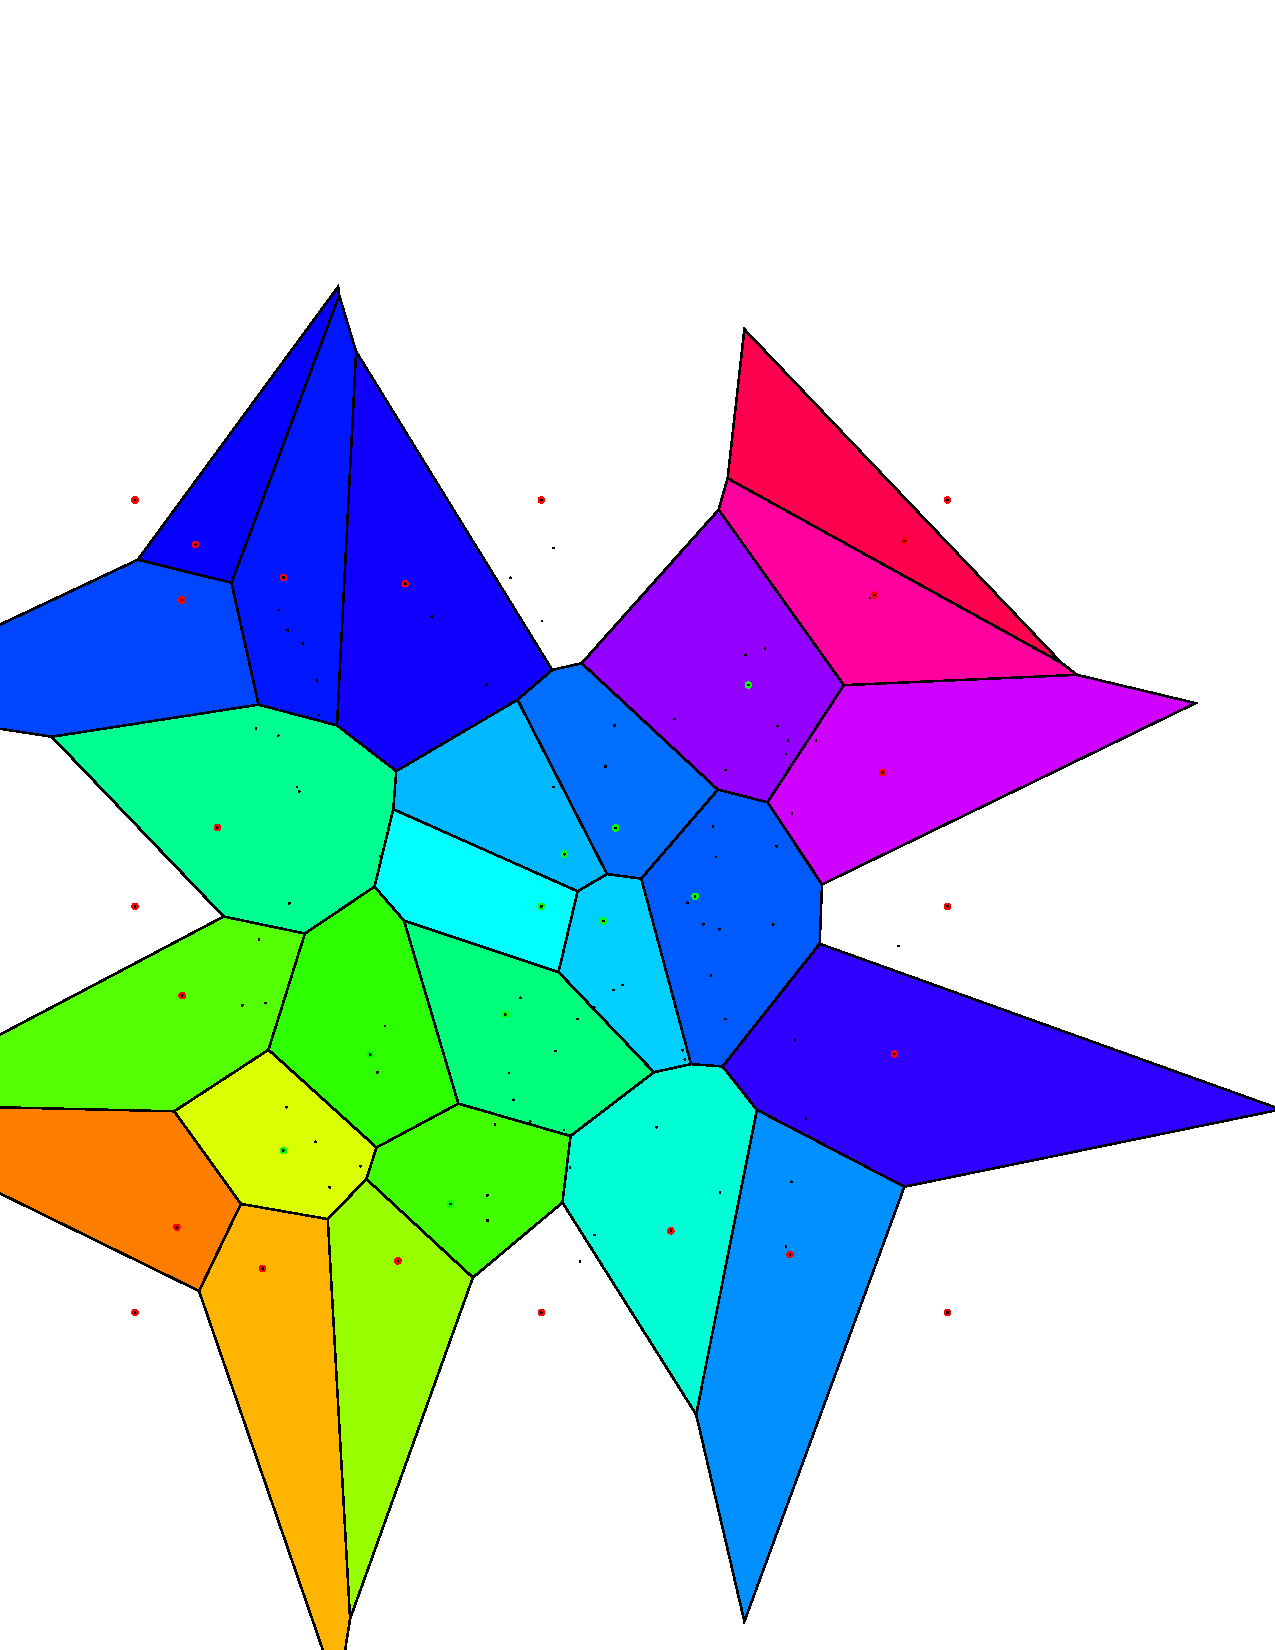
\includegraphics[trim={0 0 0 4cm},clip, width=0.45\textwidth]{../viz/100/voro9.pdf}}
   \subfloat {
\includegraphics[trim={0 0 0 4cm},clip, width=0.45\textwidth]{../viz/100/voro_err9.pdf}}
\end{figure}
%======================================================

\newpage
\begin{figure}[!tbh]
\centering           
   \subfloat {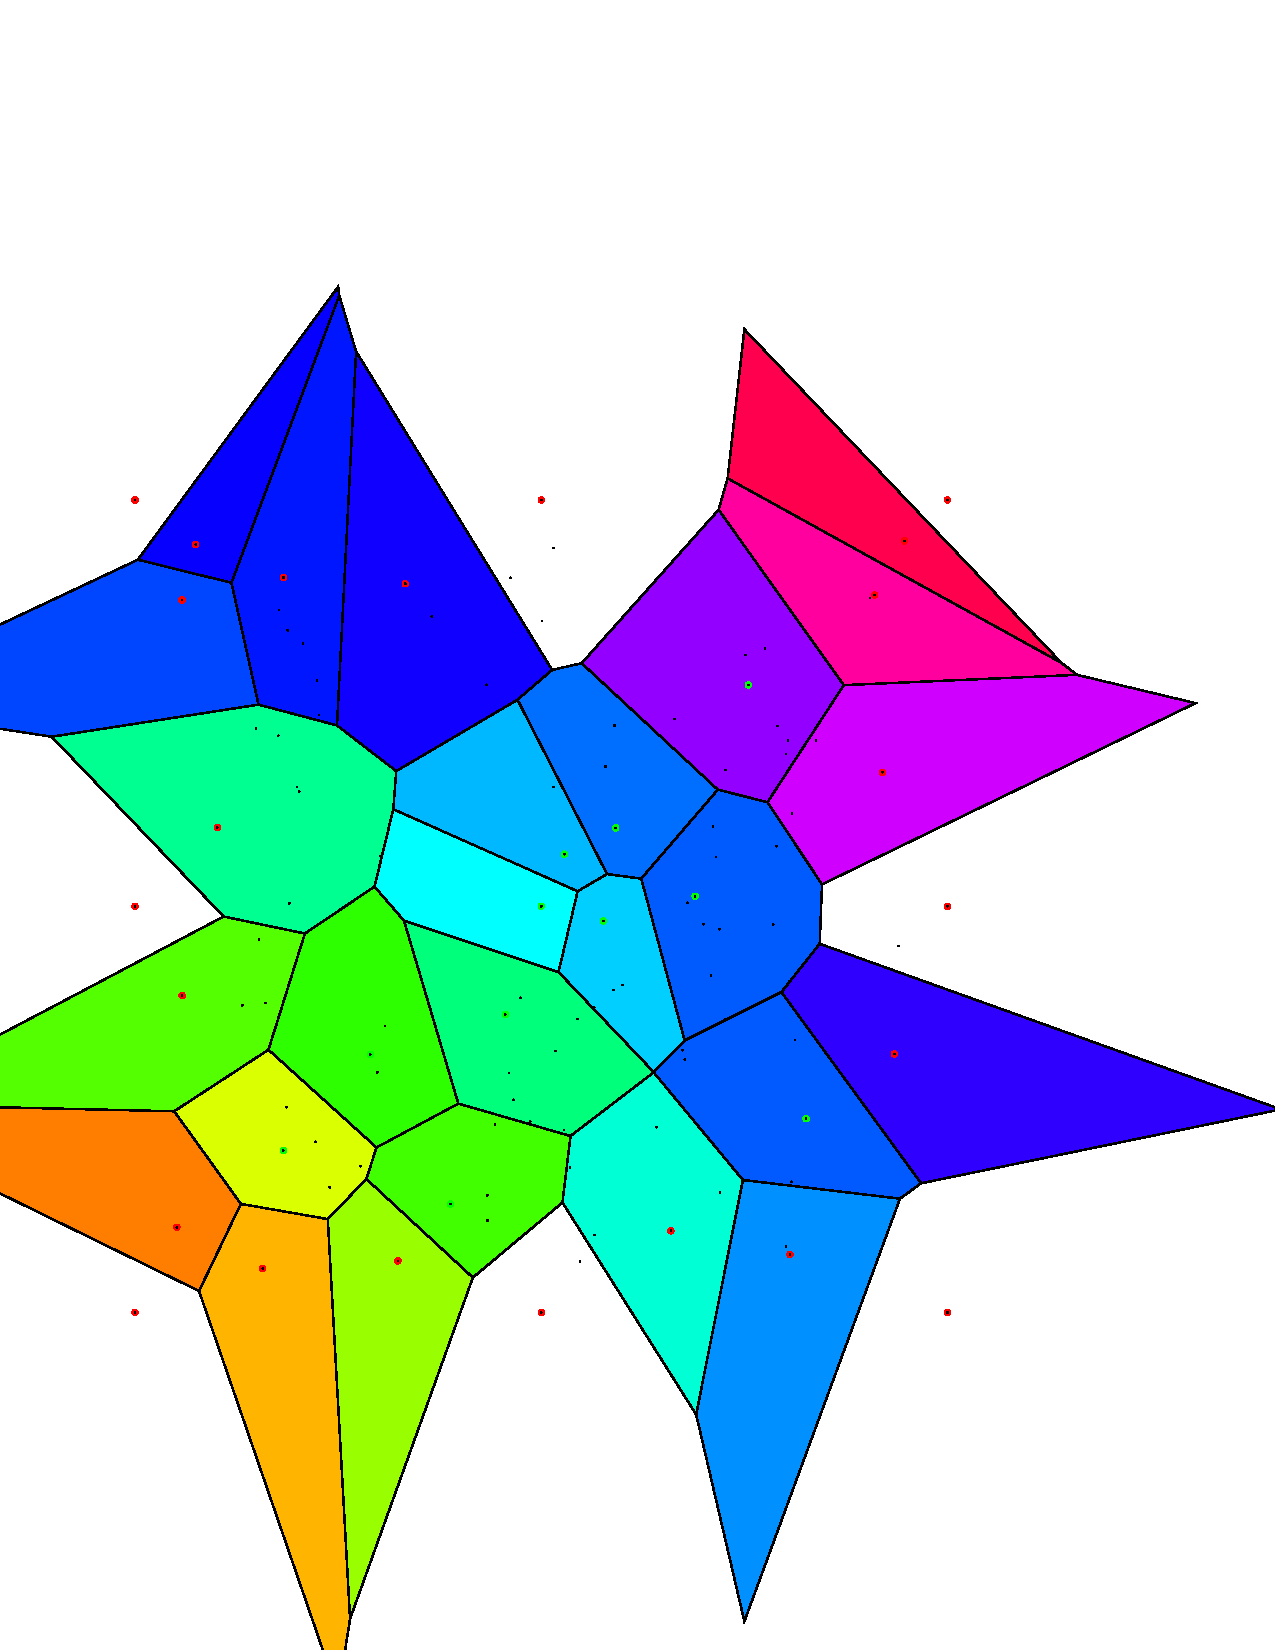
\includegraphics[trim={0 0 0 4cm},clip, width=0.45\textwidth]{../viz/100/voro10.pdf}}
   \subfloat {
\includegraphics[trim={0 0 0 4cm},clip, width=0.45\textwidth]{../viz/100/voro_err10.pdf}}
   
   \subfloat {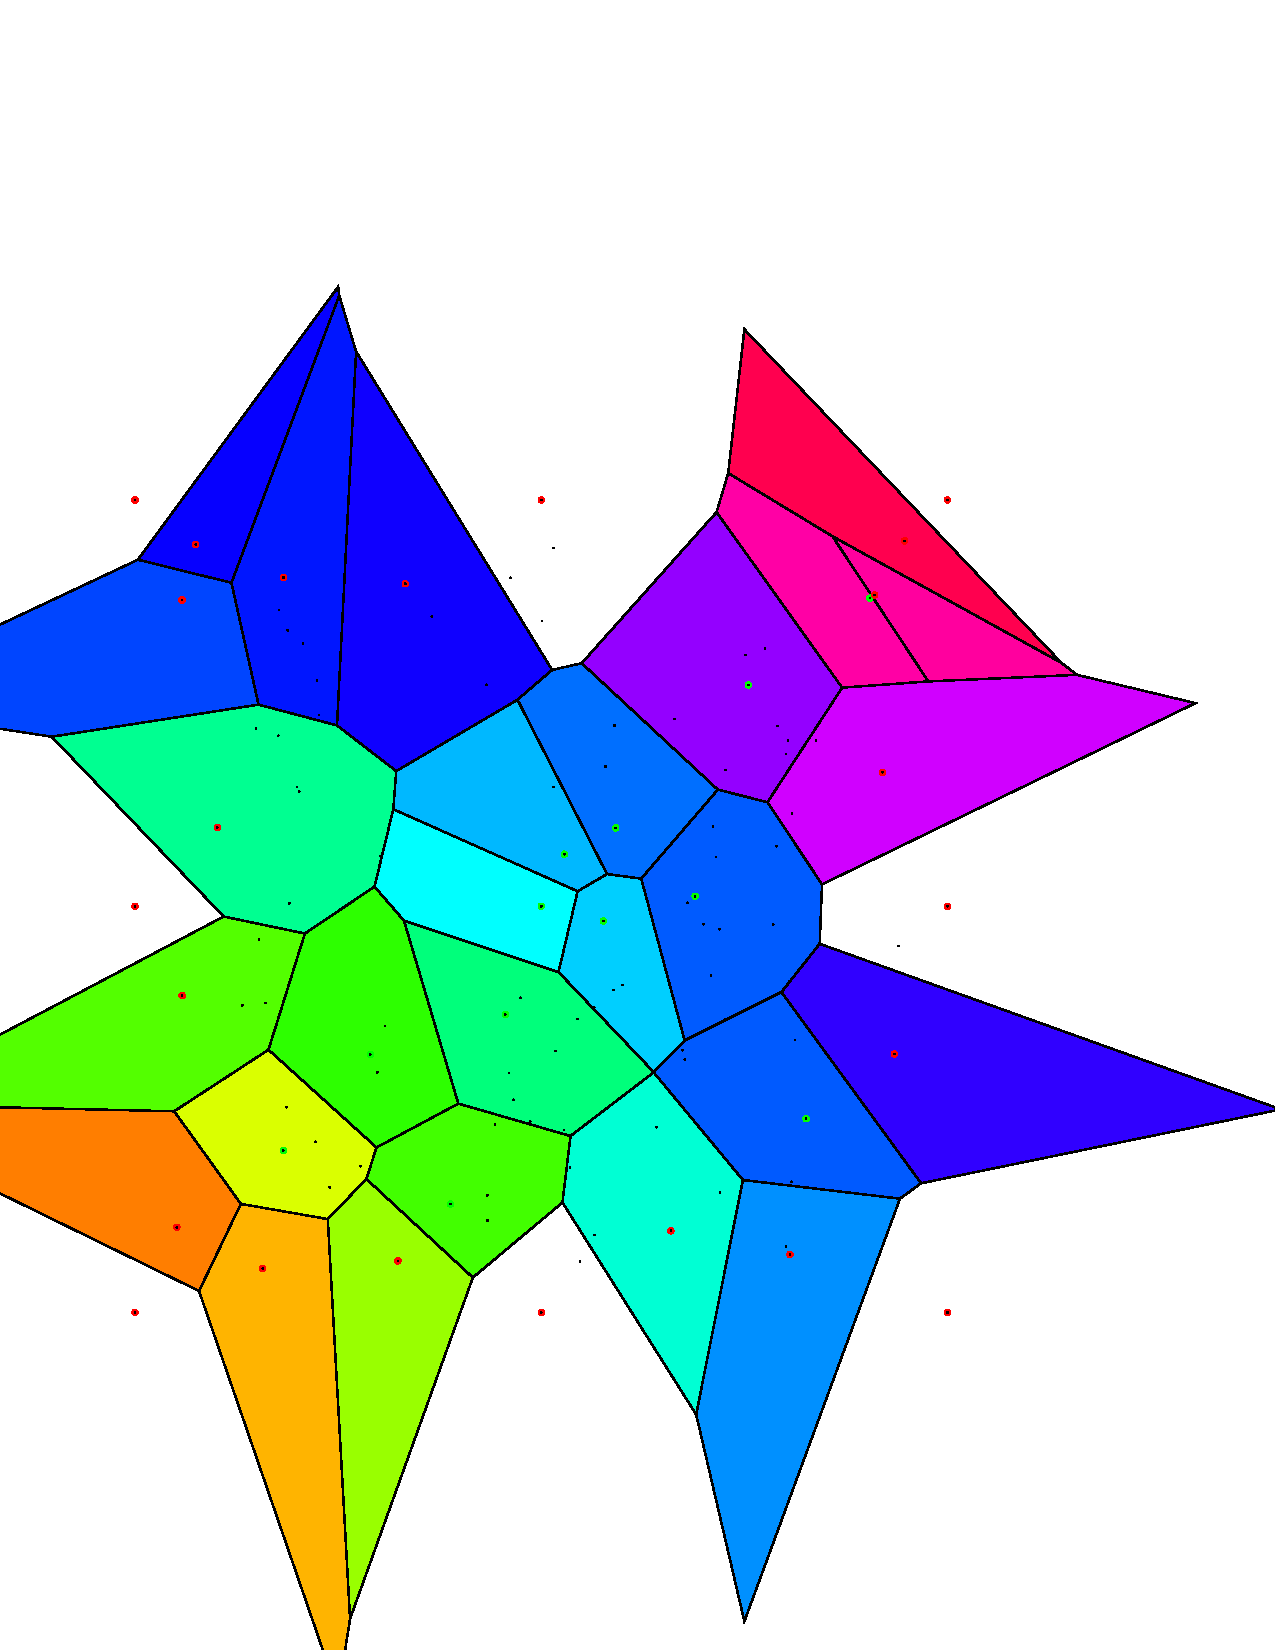
\includegraphics[trim={0 0 0 4cm},clip, width=0.45\textwidth]{../viz/100/voro11.pdf}}
   \subfloat {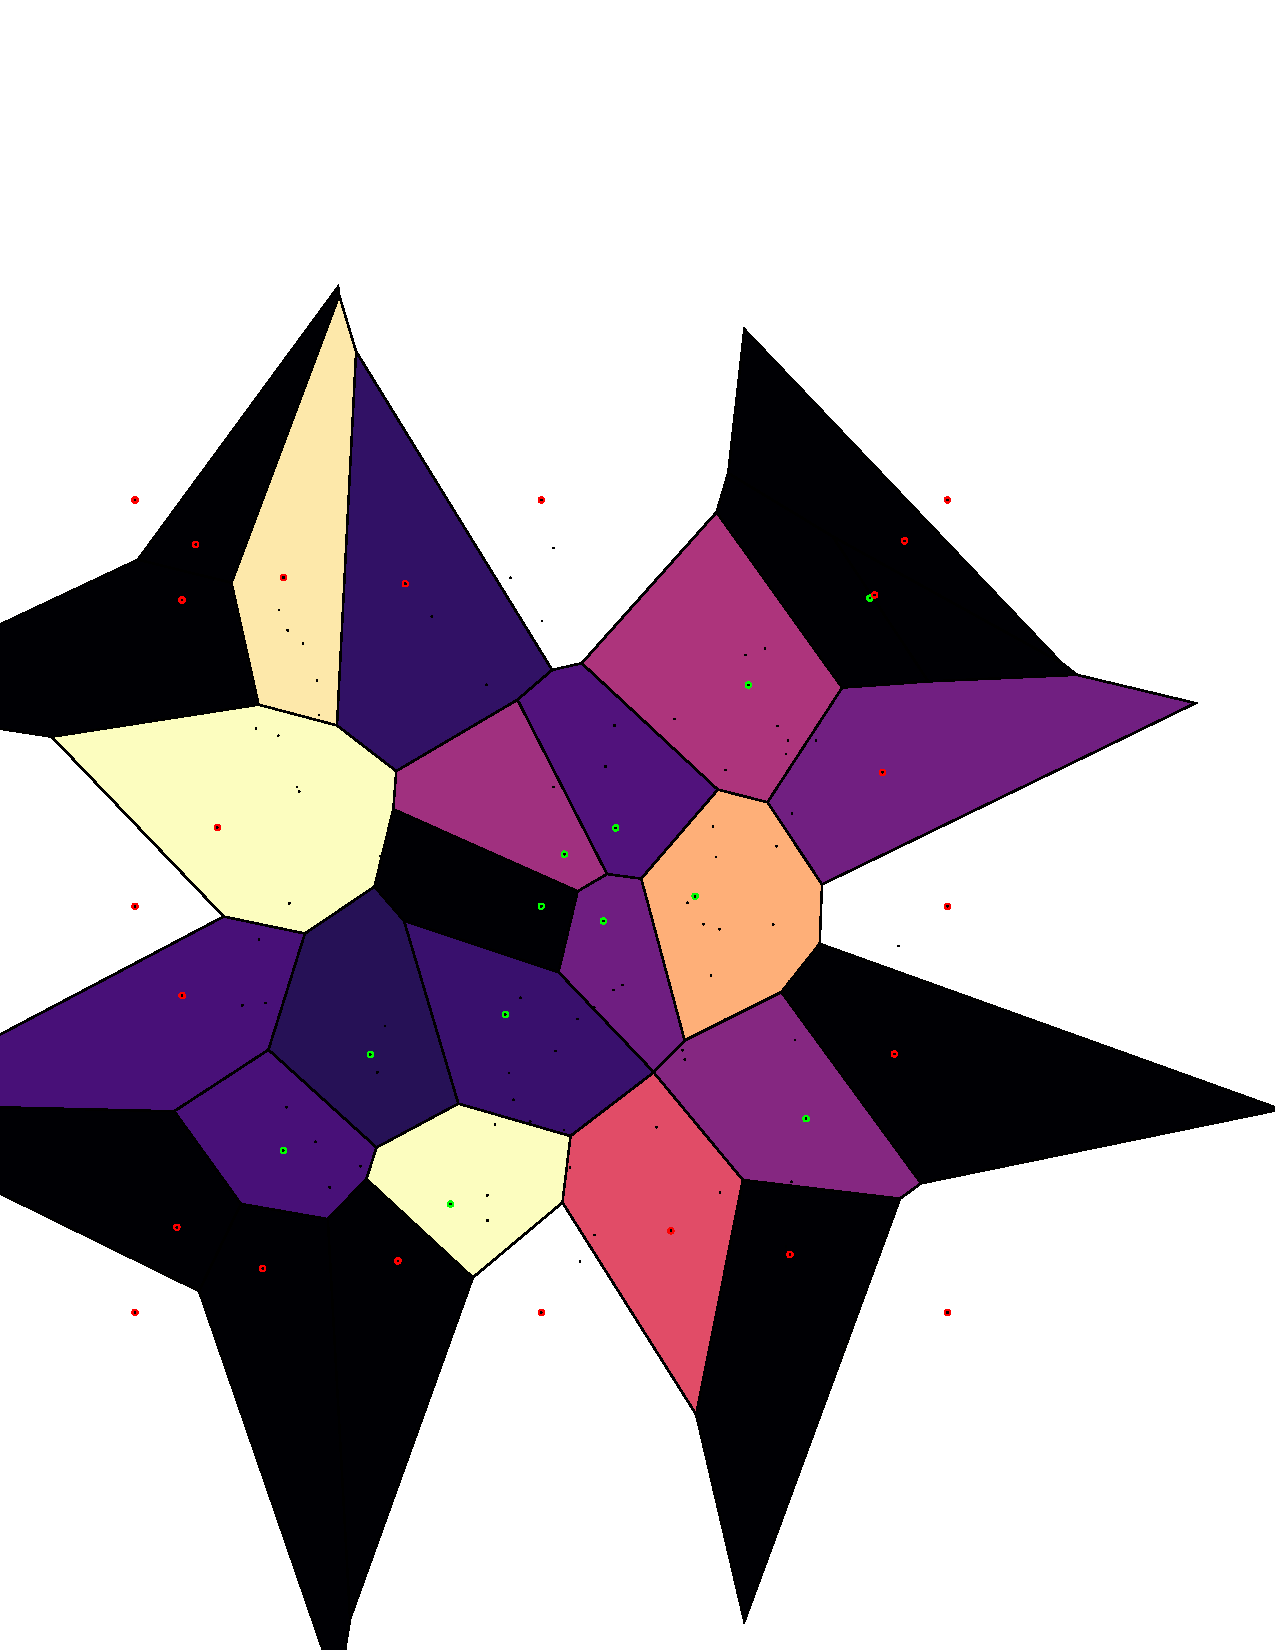
\includegraphics[trim={0 0 0 4cm},clip, width=0.45\textwidth]{../viz/100/voro_err11.pdf}}
\end{figure}
%======================================================

\newpage
\begin{figure}[!tbh]
\centering           
   \subfloat {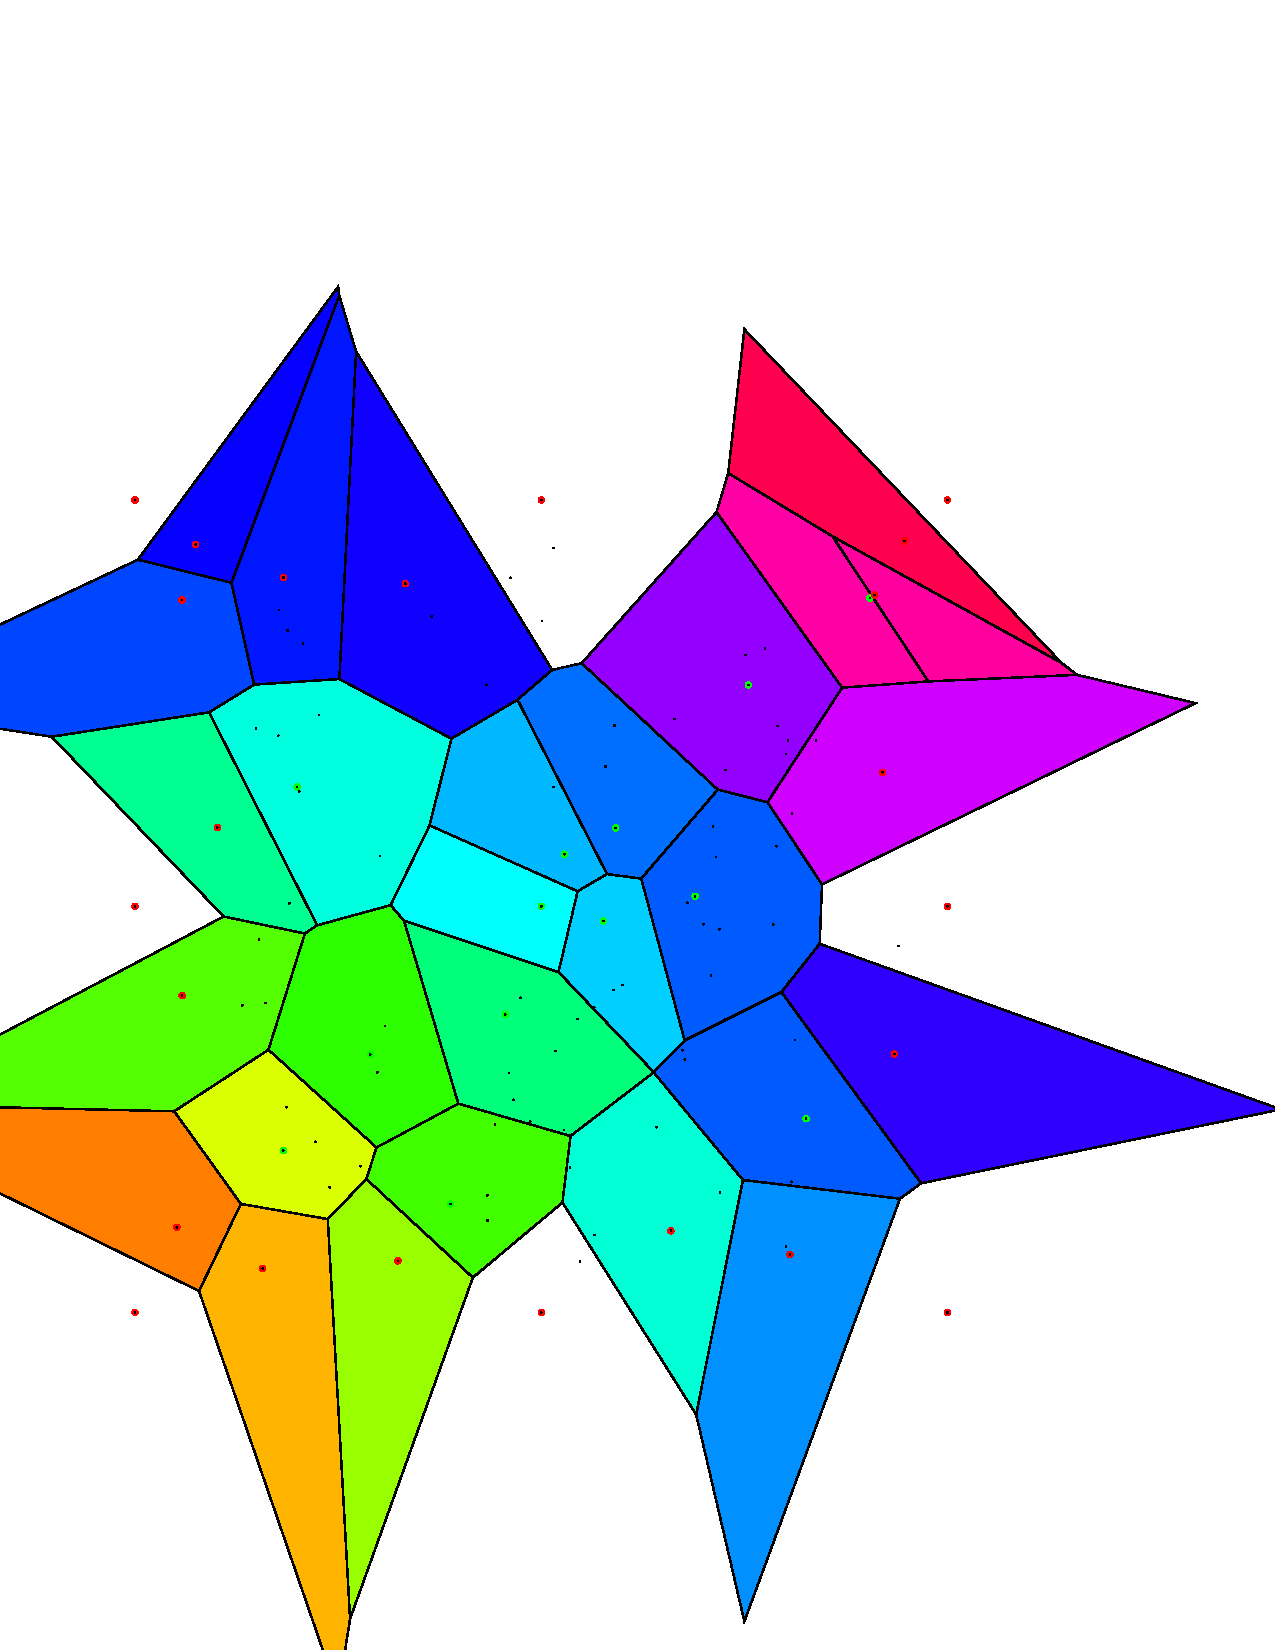
\includegraphics[trim={0 0 0 4cm},clip, width=0.45\textwidth]{../viz/100/voro12.pdf}}
   \subfloat {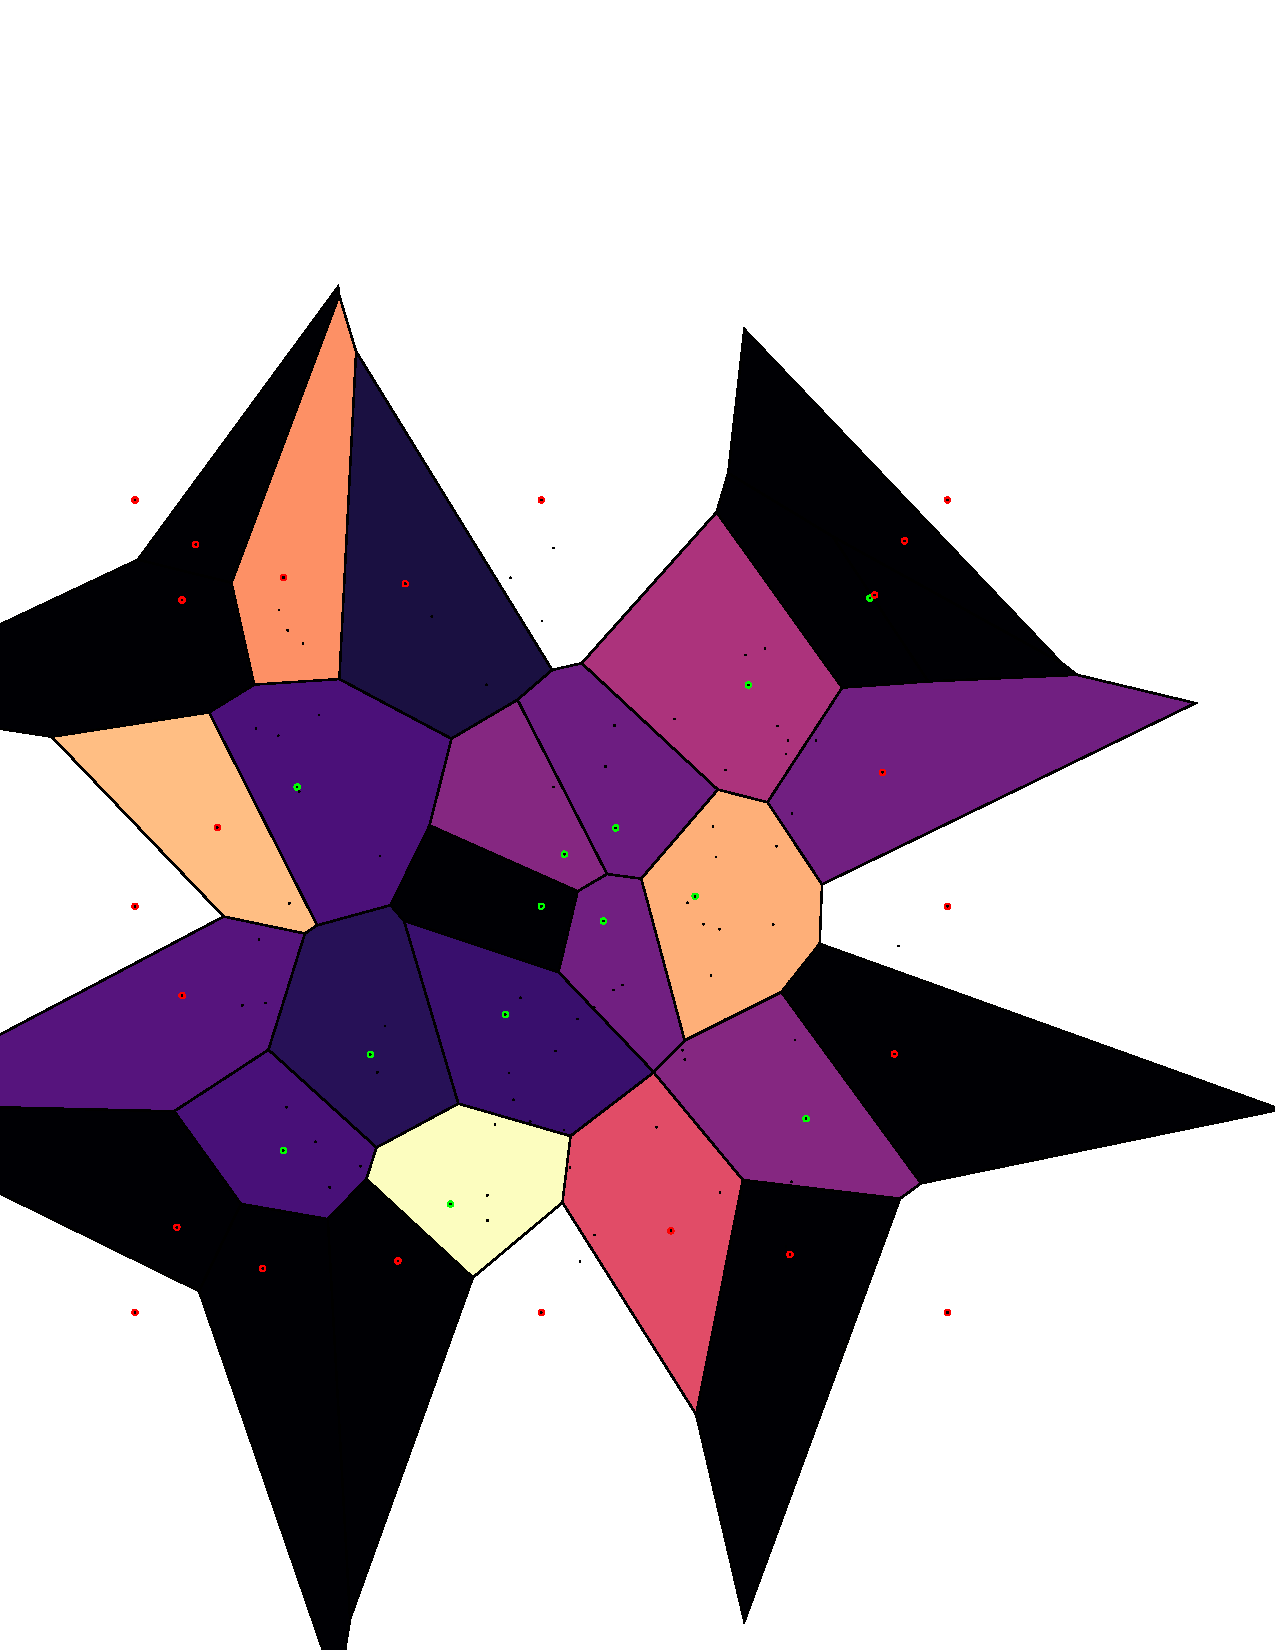
\includegraphics[trim={0 0 0 4cm},clip, width=0.45\textwidth]{../viz/100/voro_err12.pdf}}
   
   \subfloat {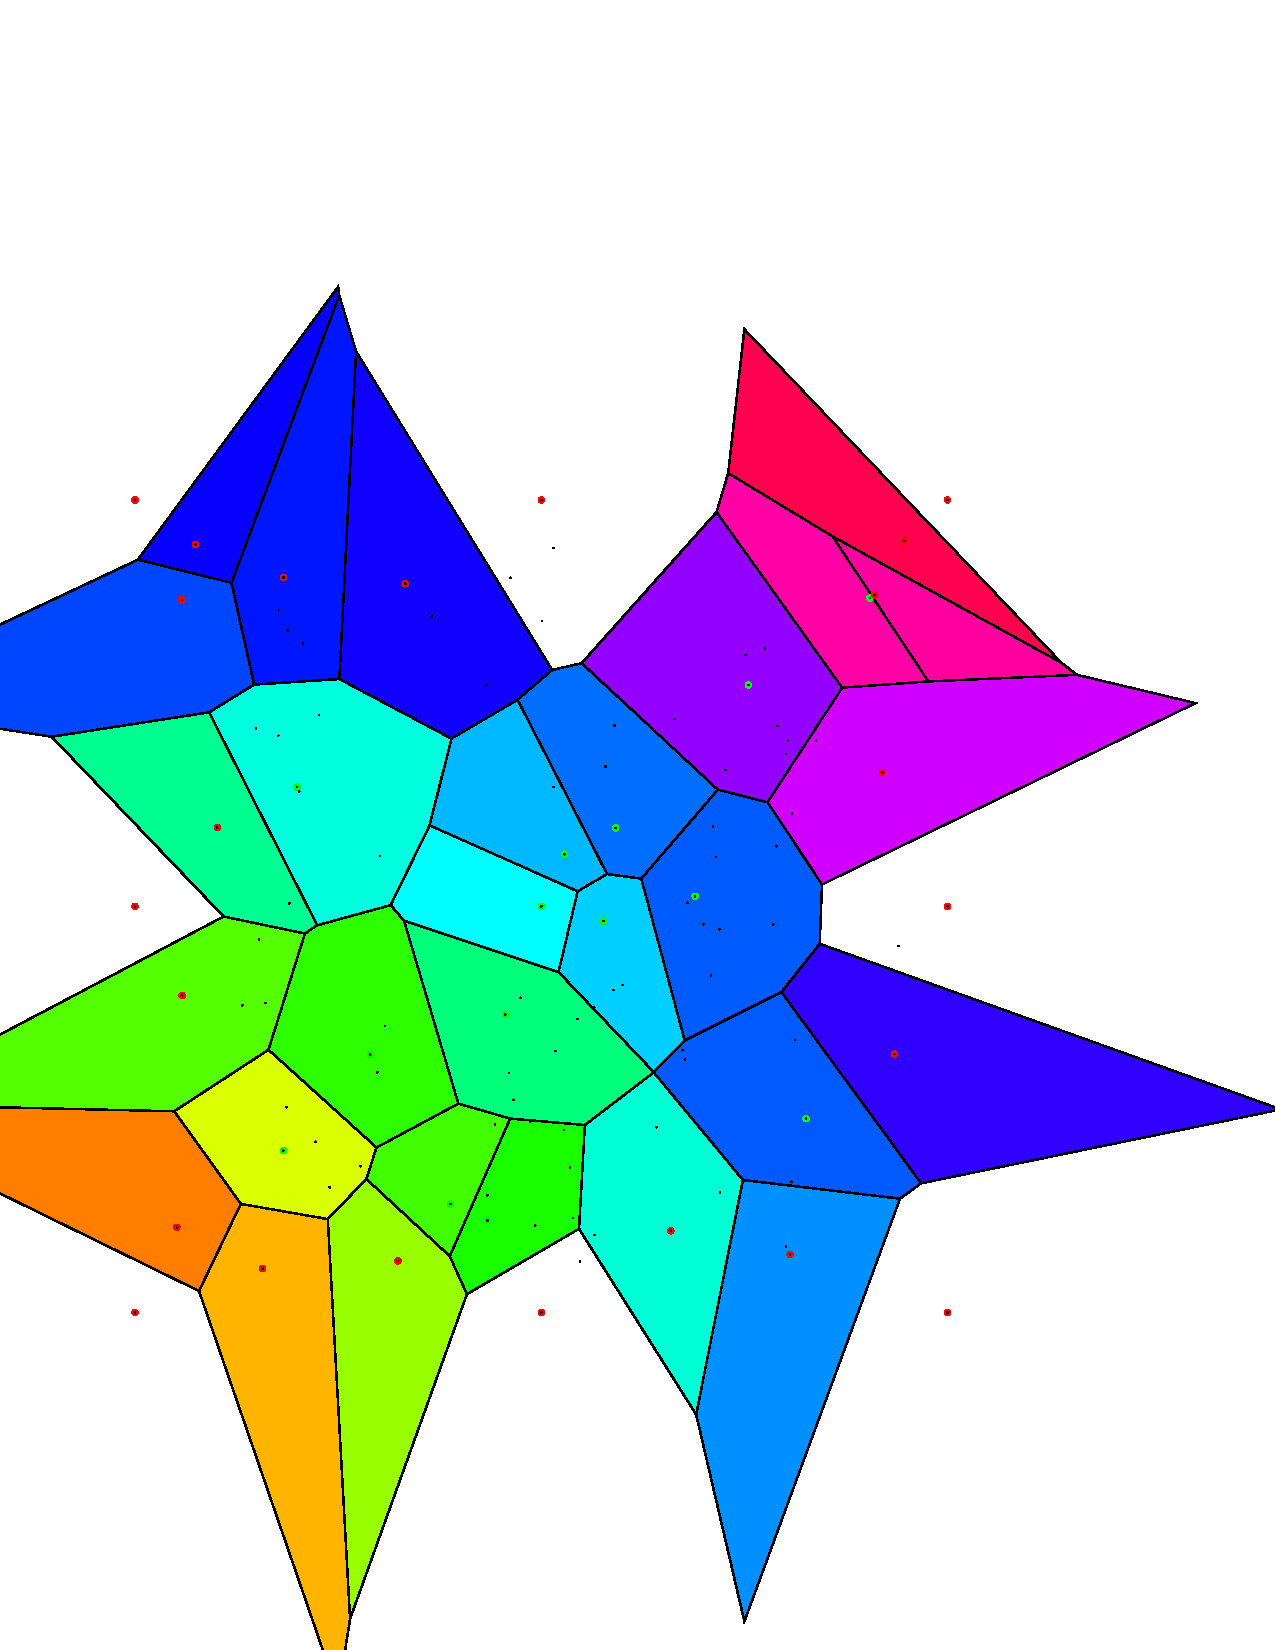
\includegraphics[trim={0 0 0 4cm},clip, width=0.45\textwidth]{../viz/100/voro13.pdf}}
   \subfloat {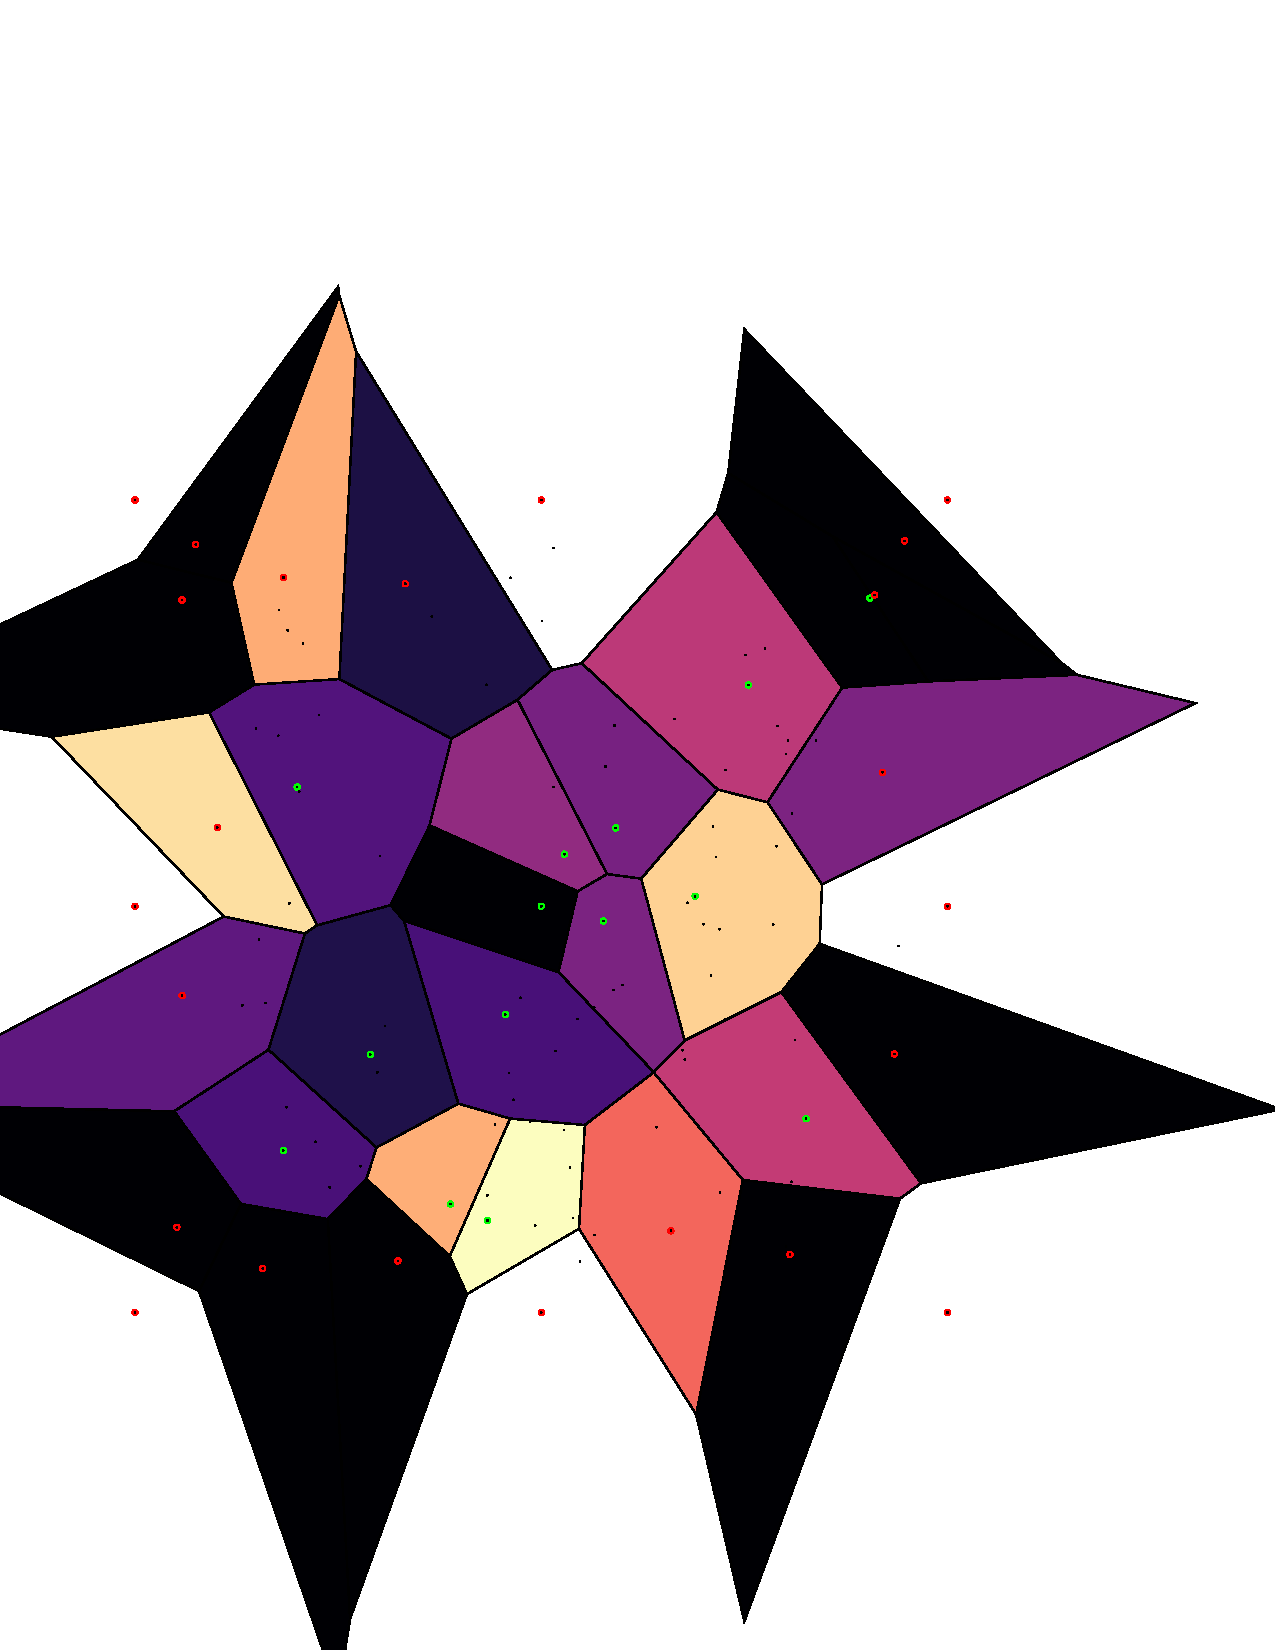
\includegraphics[trim={0 0 0 4cm},clip, width=0.45\textwidth]{../viz/100/voro_err13.pdf}}
\end{figure}
%======================================================

\newpage
\begin{figure}[!tbh]
\centering           
   \subfloat {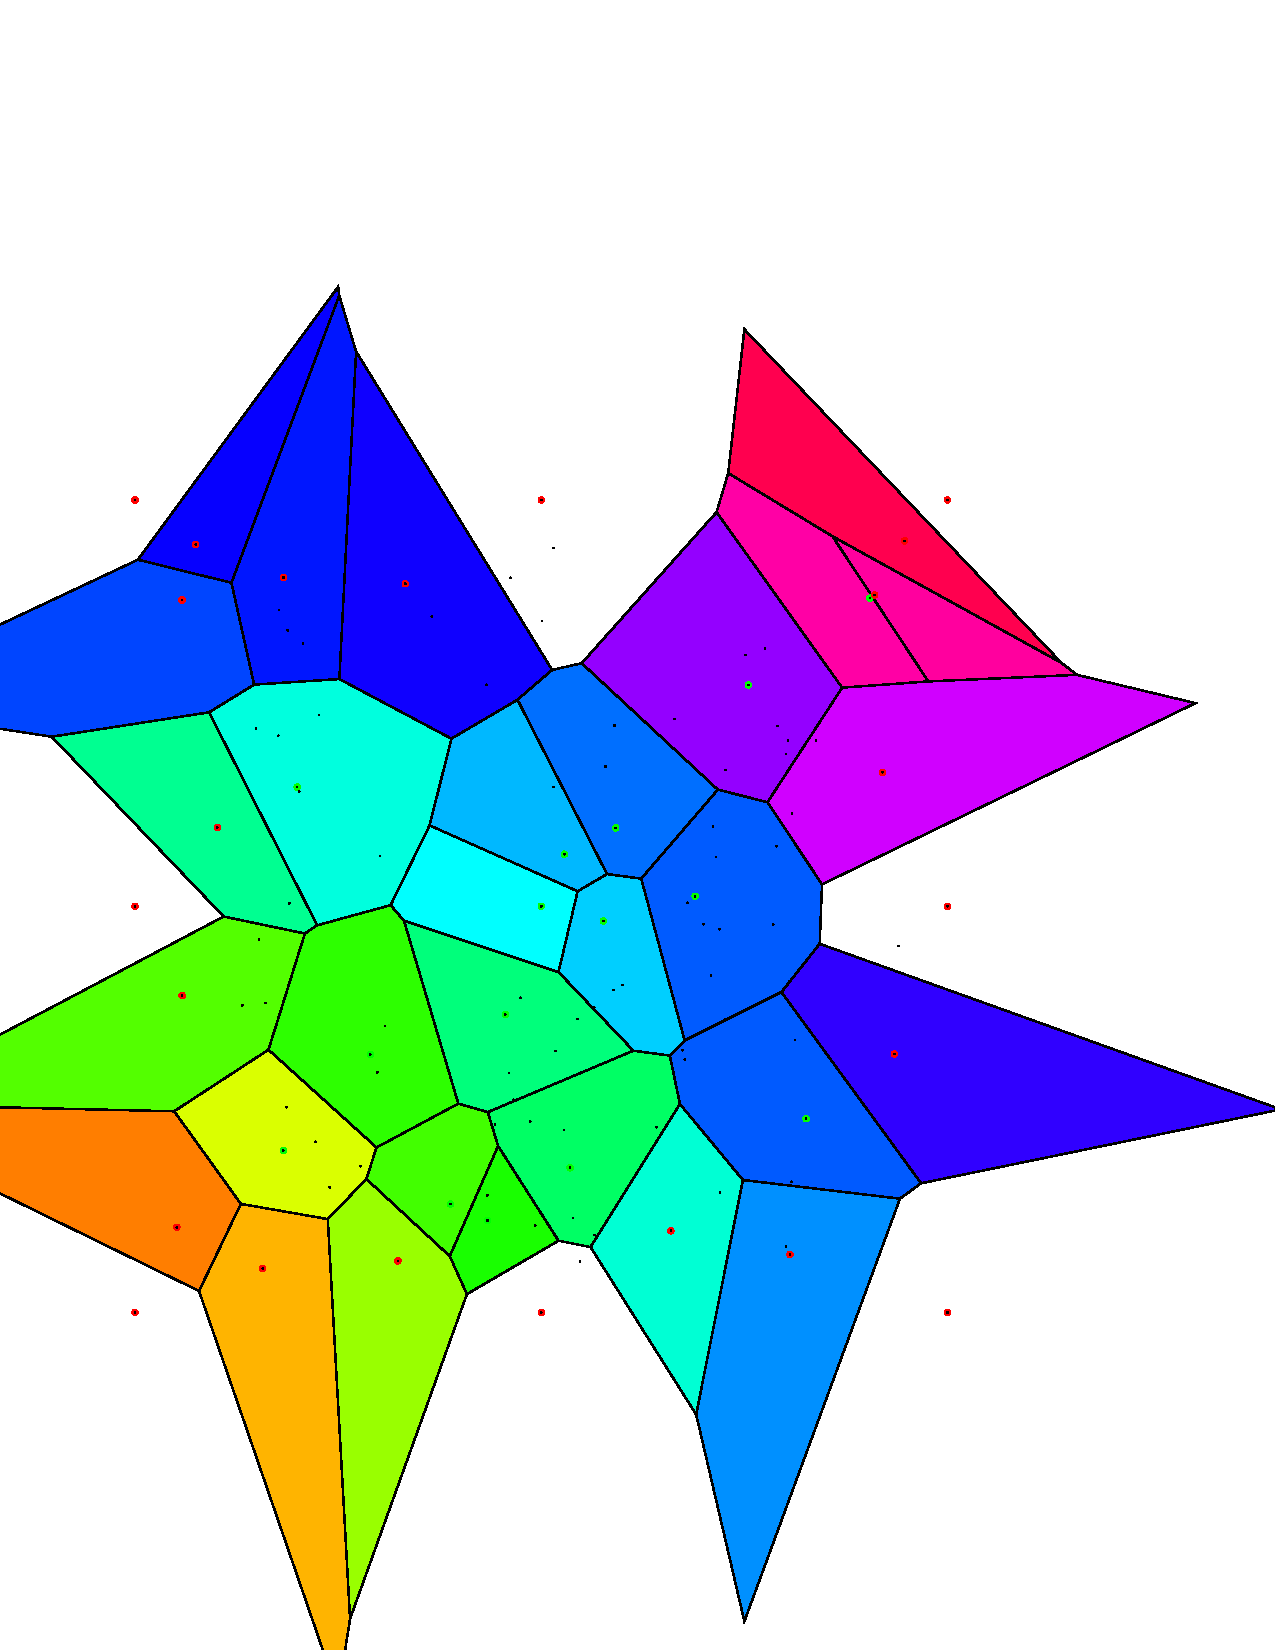
\includegraphics[trim={0 0 0 4cm},clip, width=0.45\textwidth]{../viz/100/voro14.pdf}}
   \subfloat {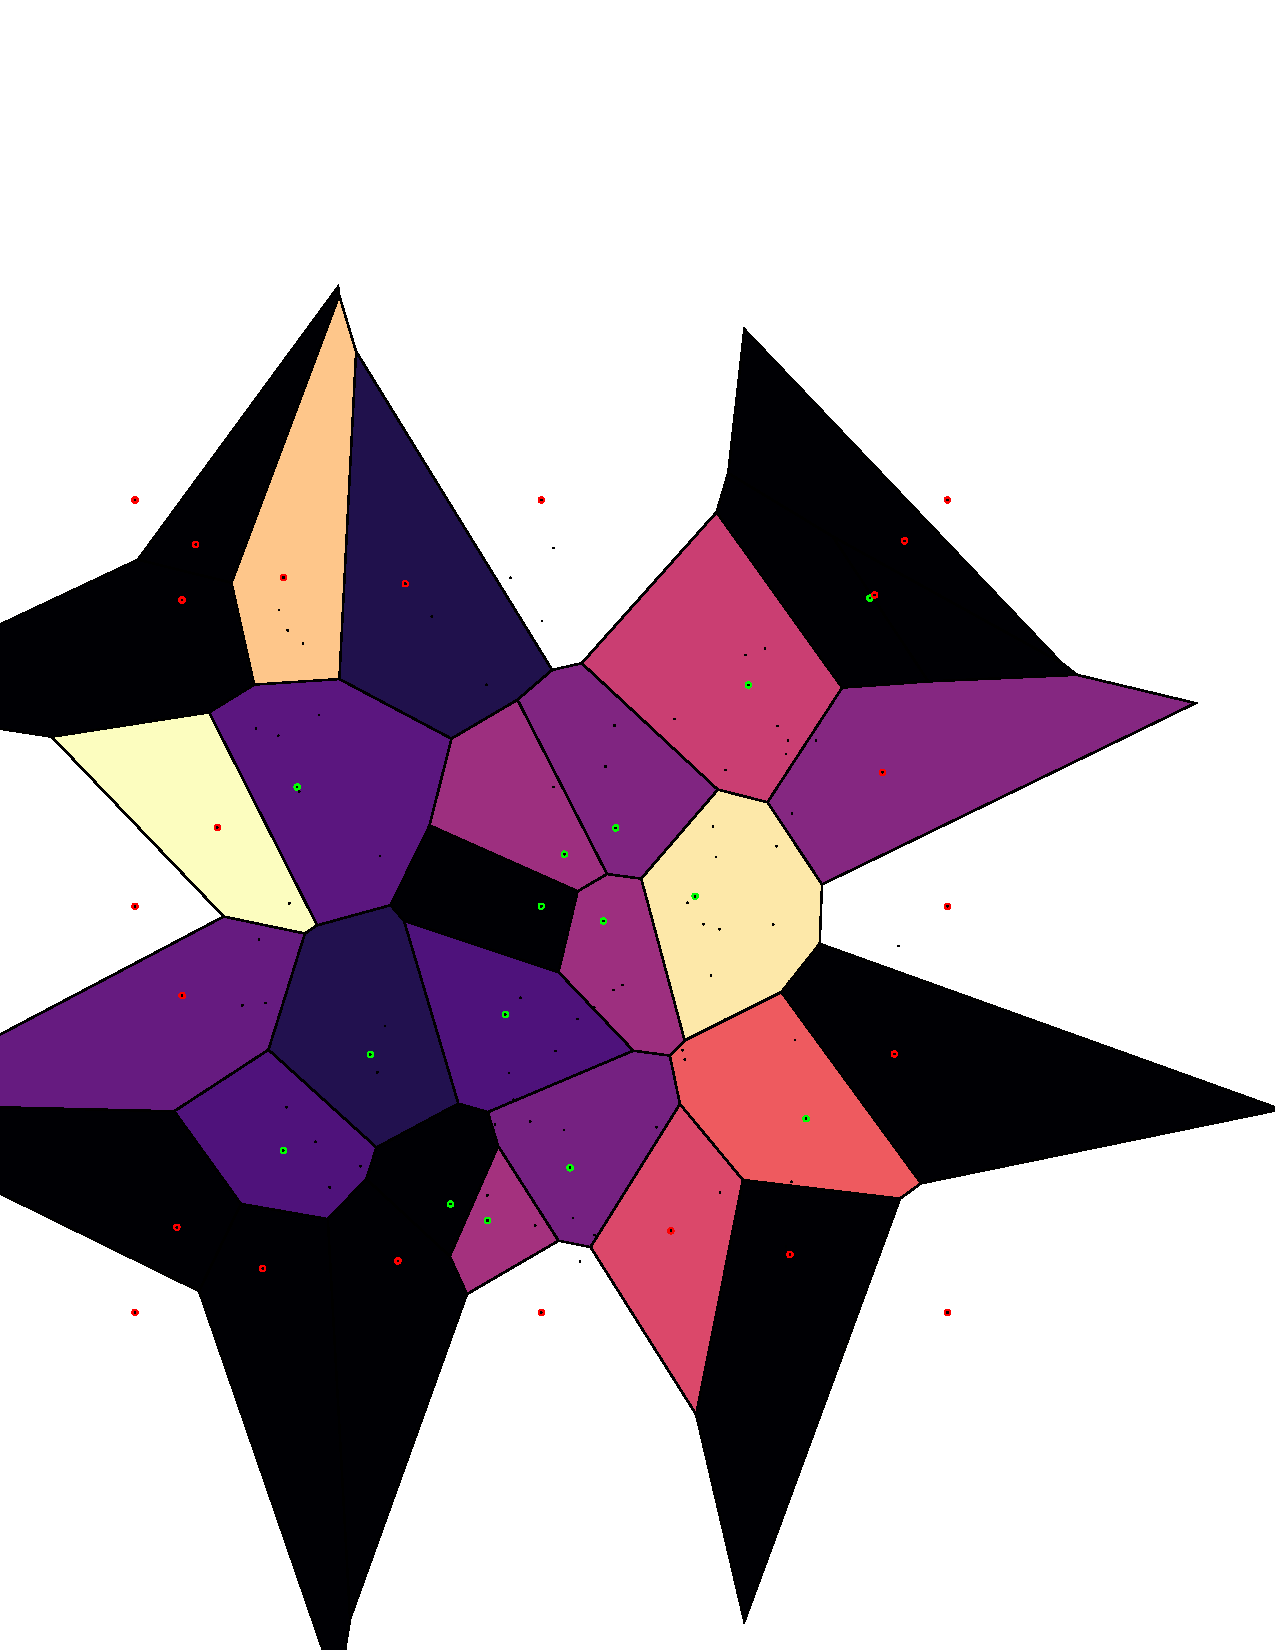
\includegraphics[trim={0 0 0 4cm},clip, width=0.45\textwidth]{../viz/100/voro_err14.pdf}}
   
   \subfloat {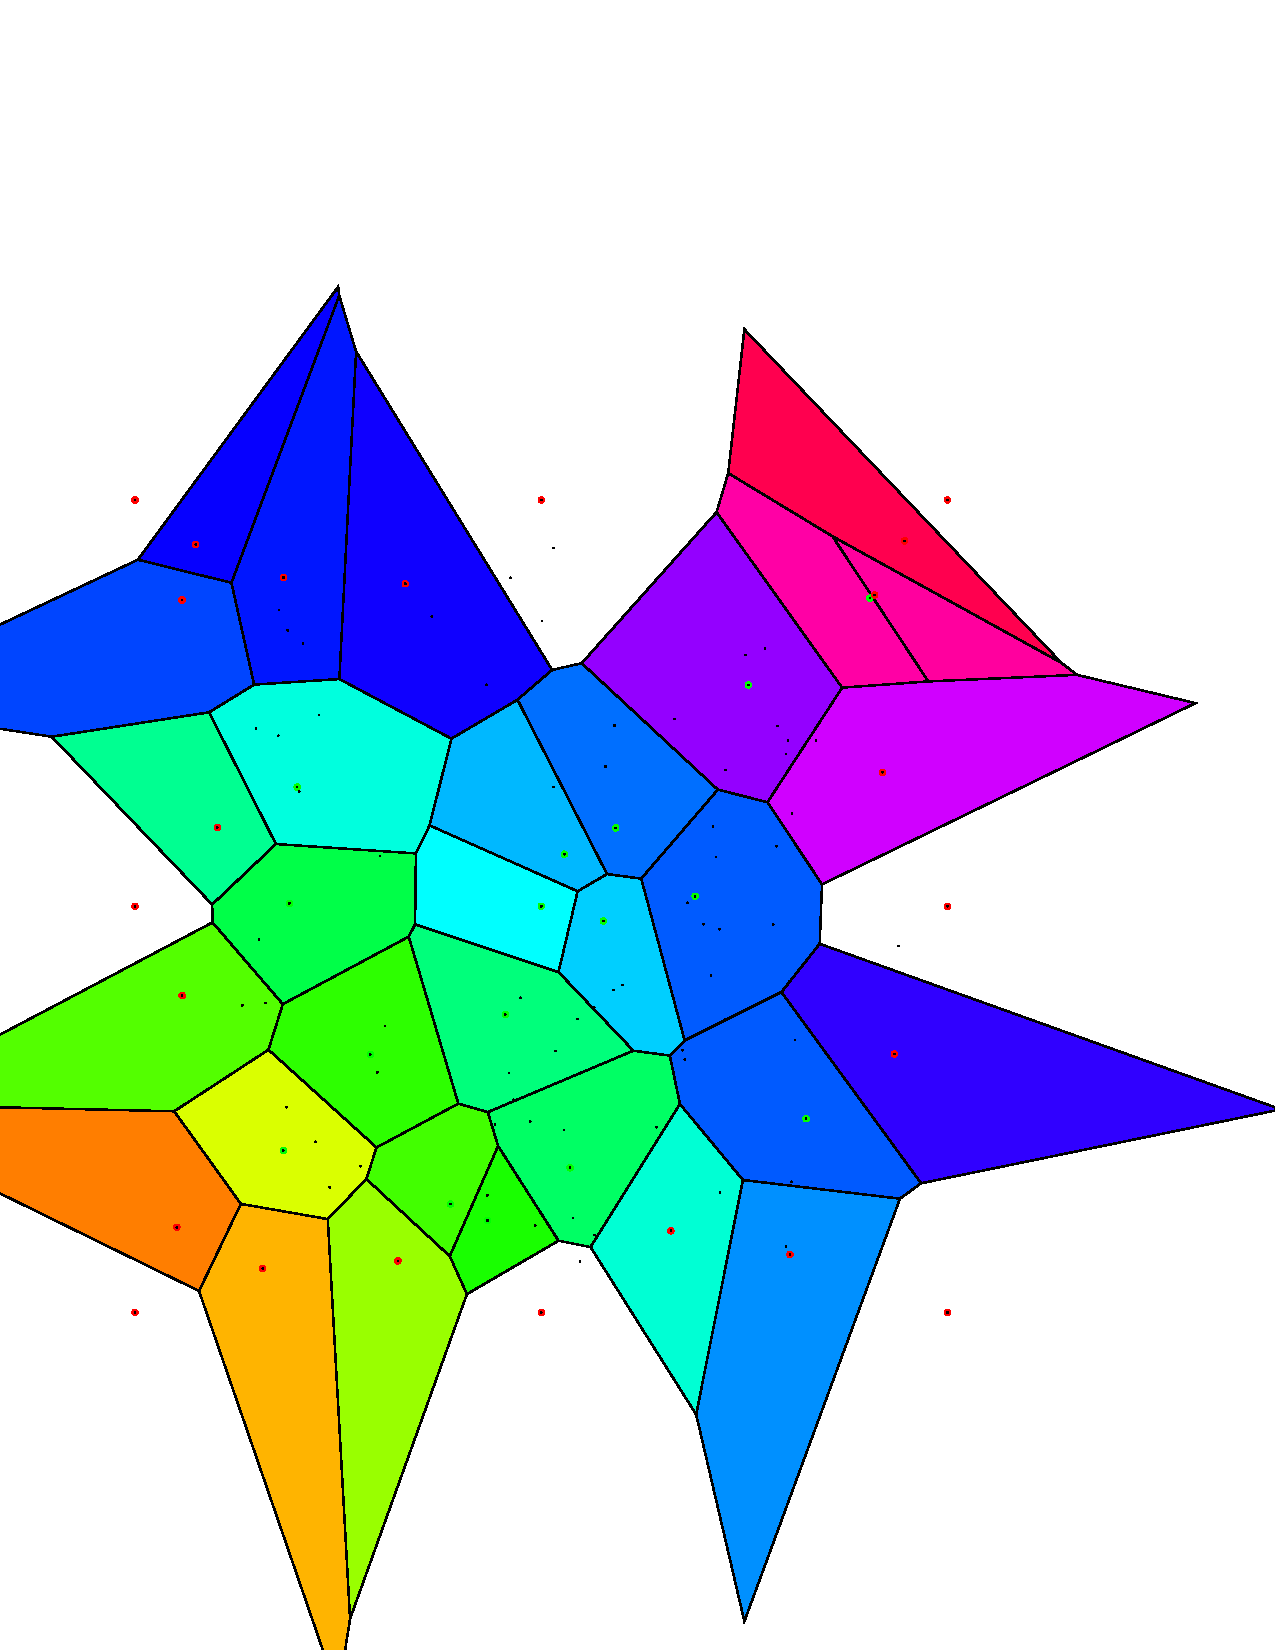
\includegraphics[trim={0 0 0 4cm},clip, width=0.45\textwidth]{../viz/100/voro15.pdf}}
   \subfloat {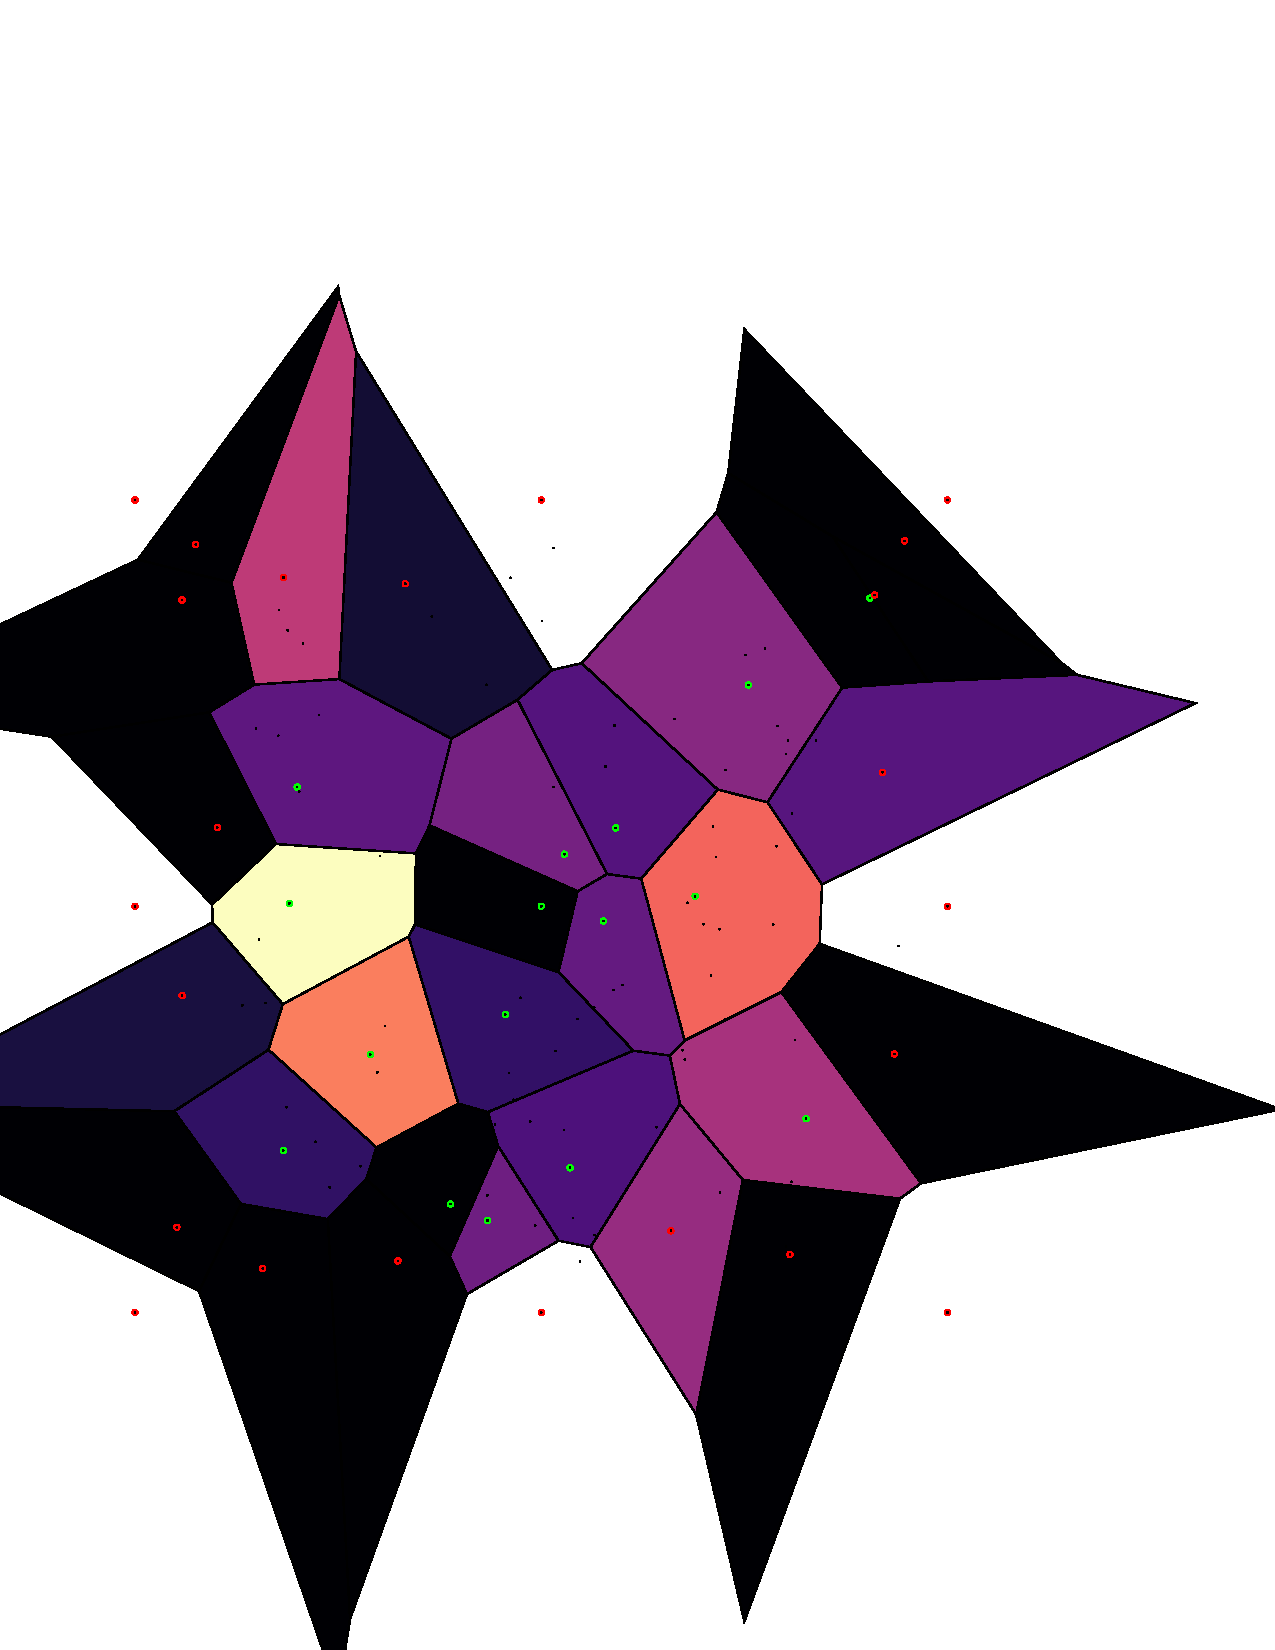
\includegraphics[trim={0 0 0 4cm},clip, width=0.45\textwidth]{../viz/100/voro_err15.pdf}}
\end{figure}
%======================================================

\newpage
\begin{figure}[!tbh]
\centering           
   \subfloat {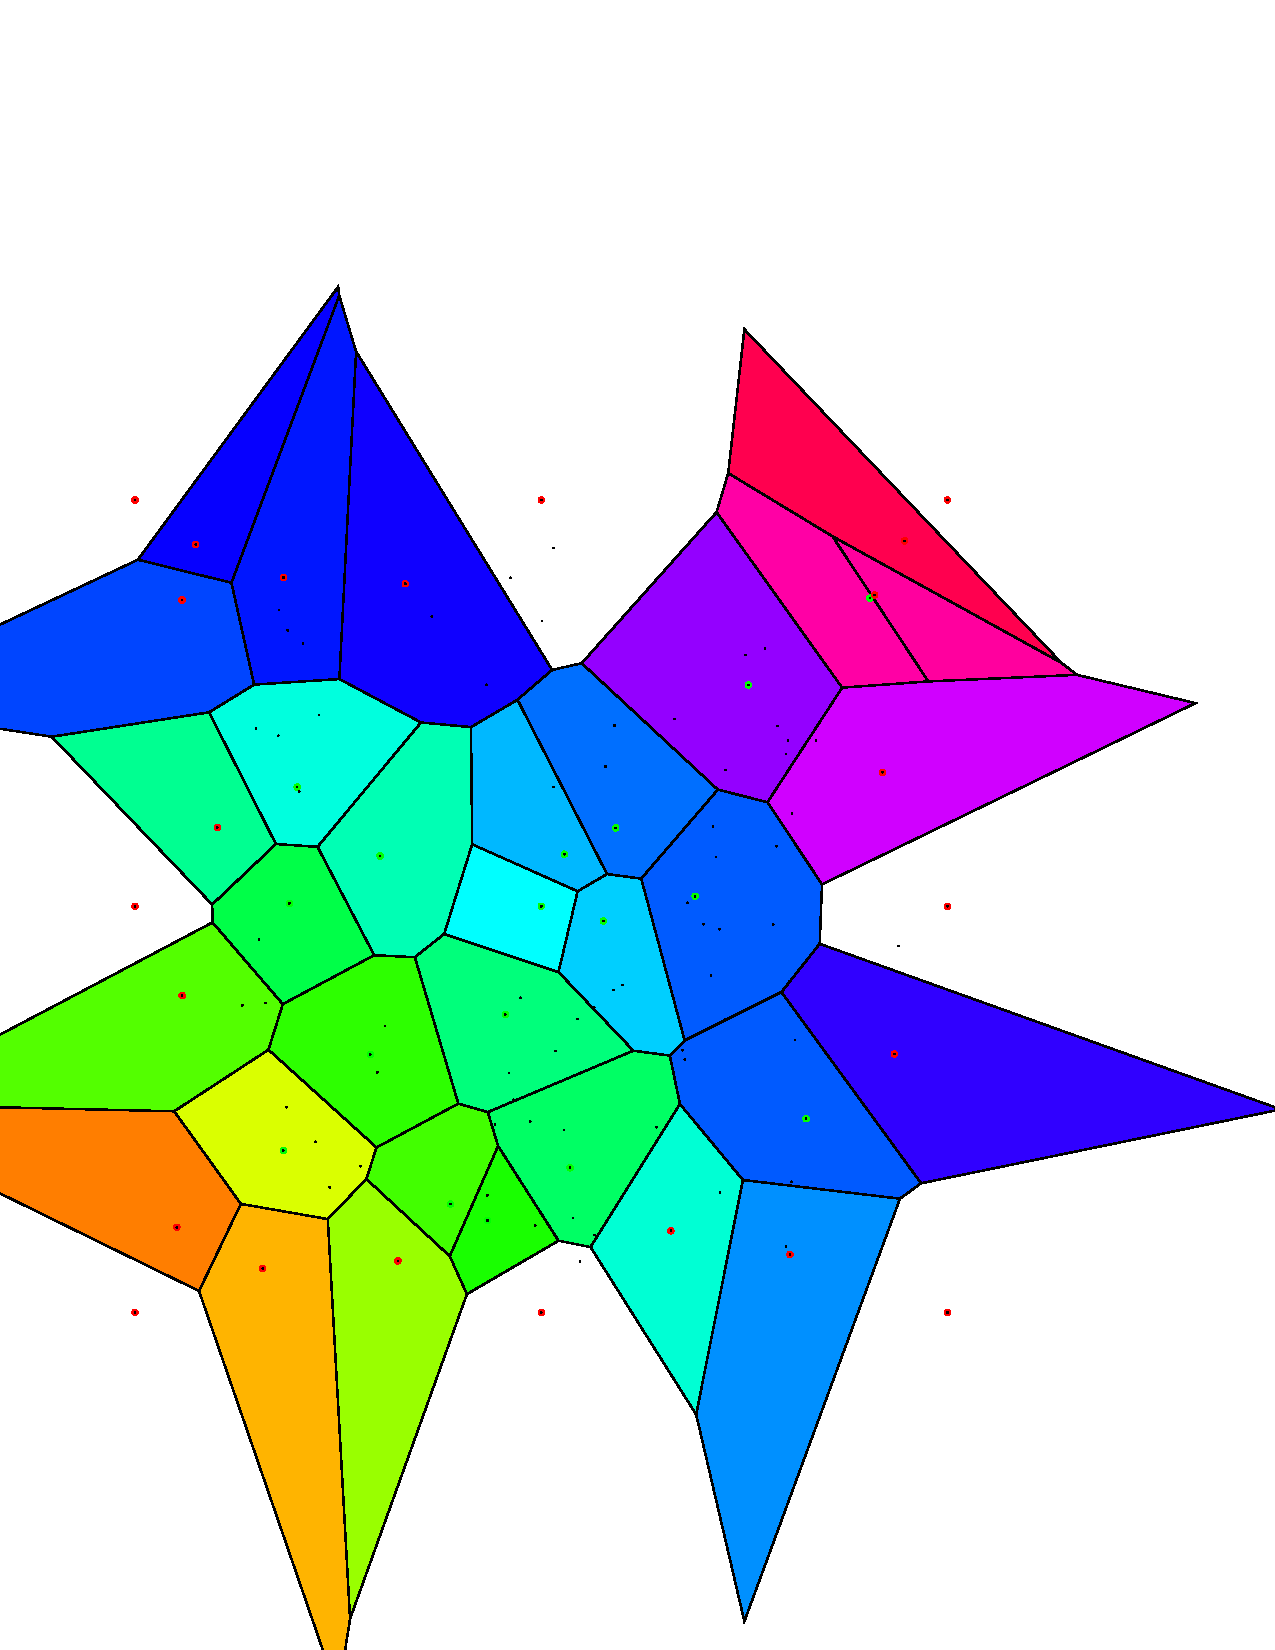
\includegraphics[trim={0 0 0 4cm},clip, width=0.45\textwidth]{../viz/100/voro16.pdf}}
   \subfloat {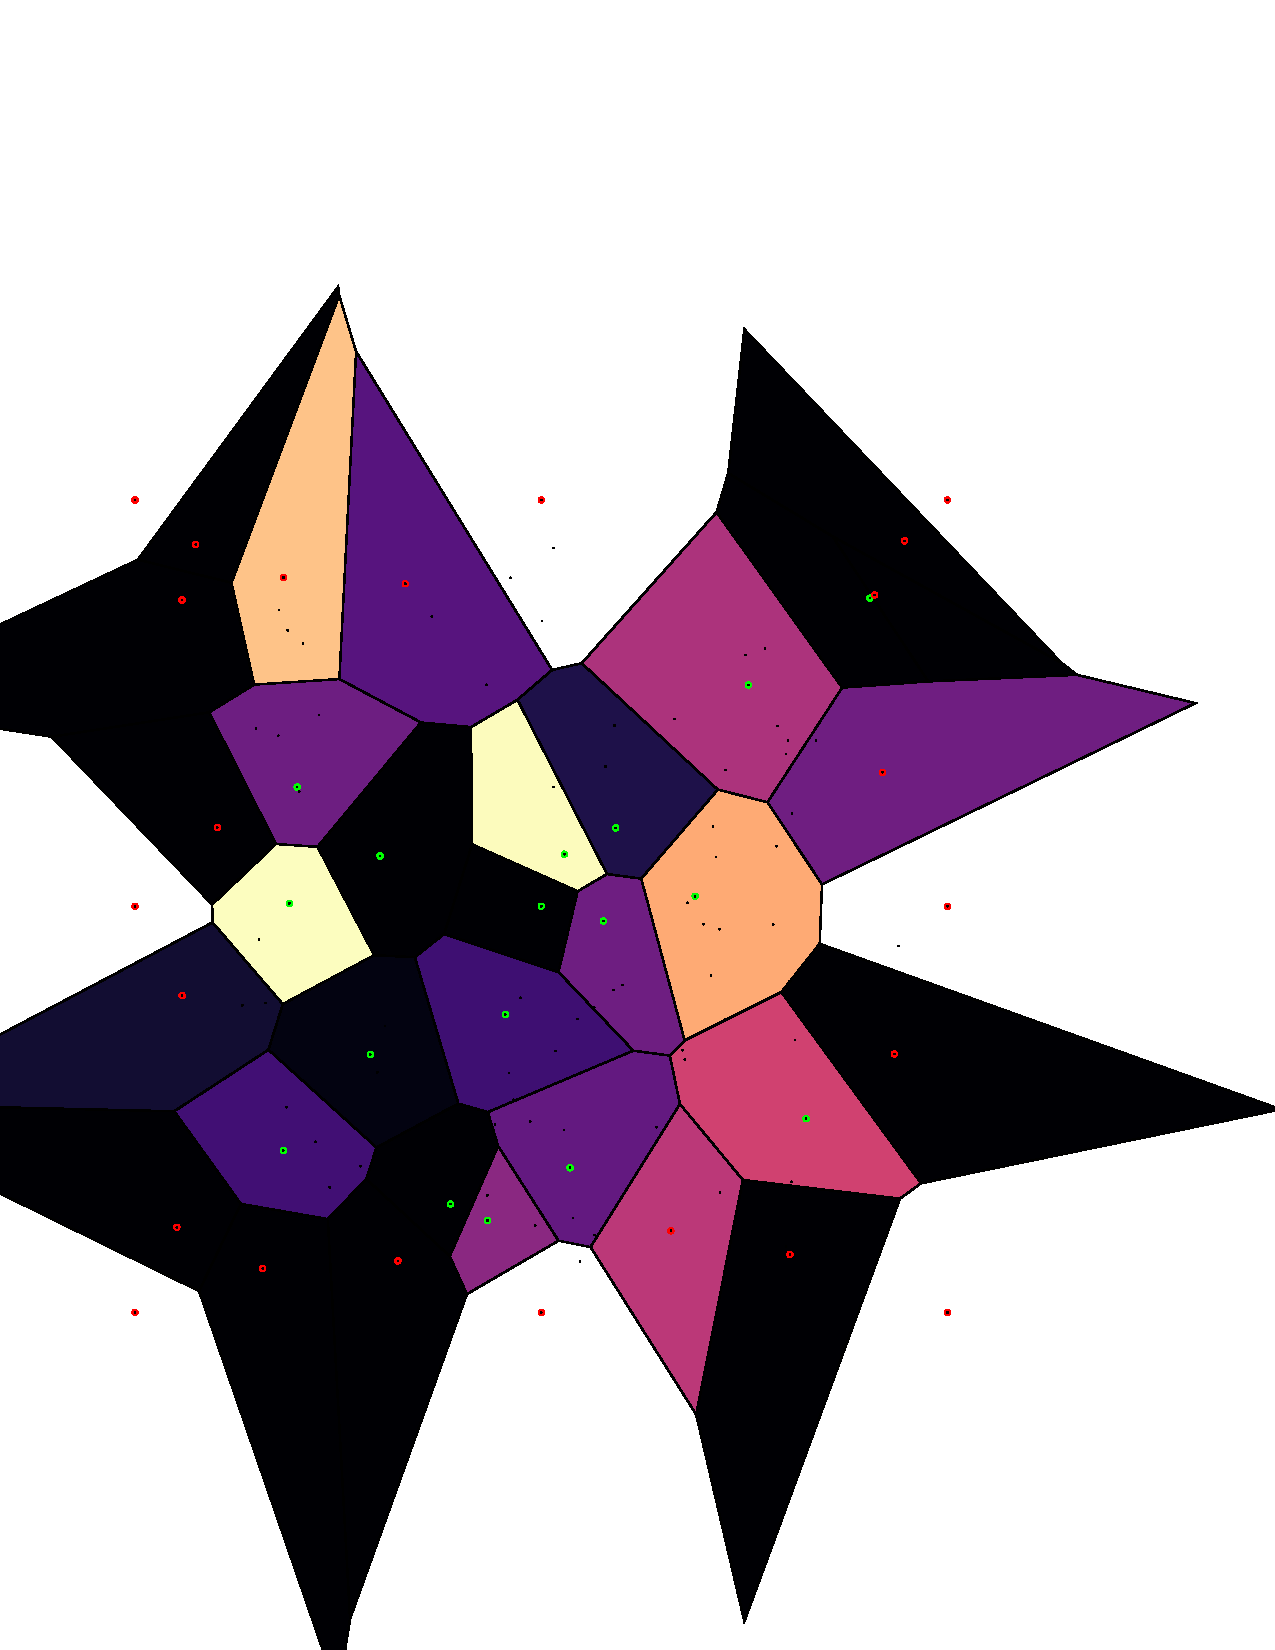
\includegraphics[trim={0 0 0 4cm},clip, width=0.45\textwidth]{../viz/100/voro_err16.pdf}}
   
   \subfloat {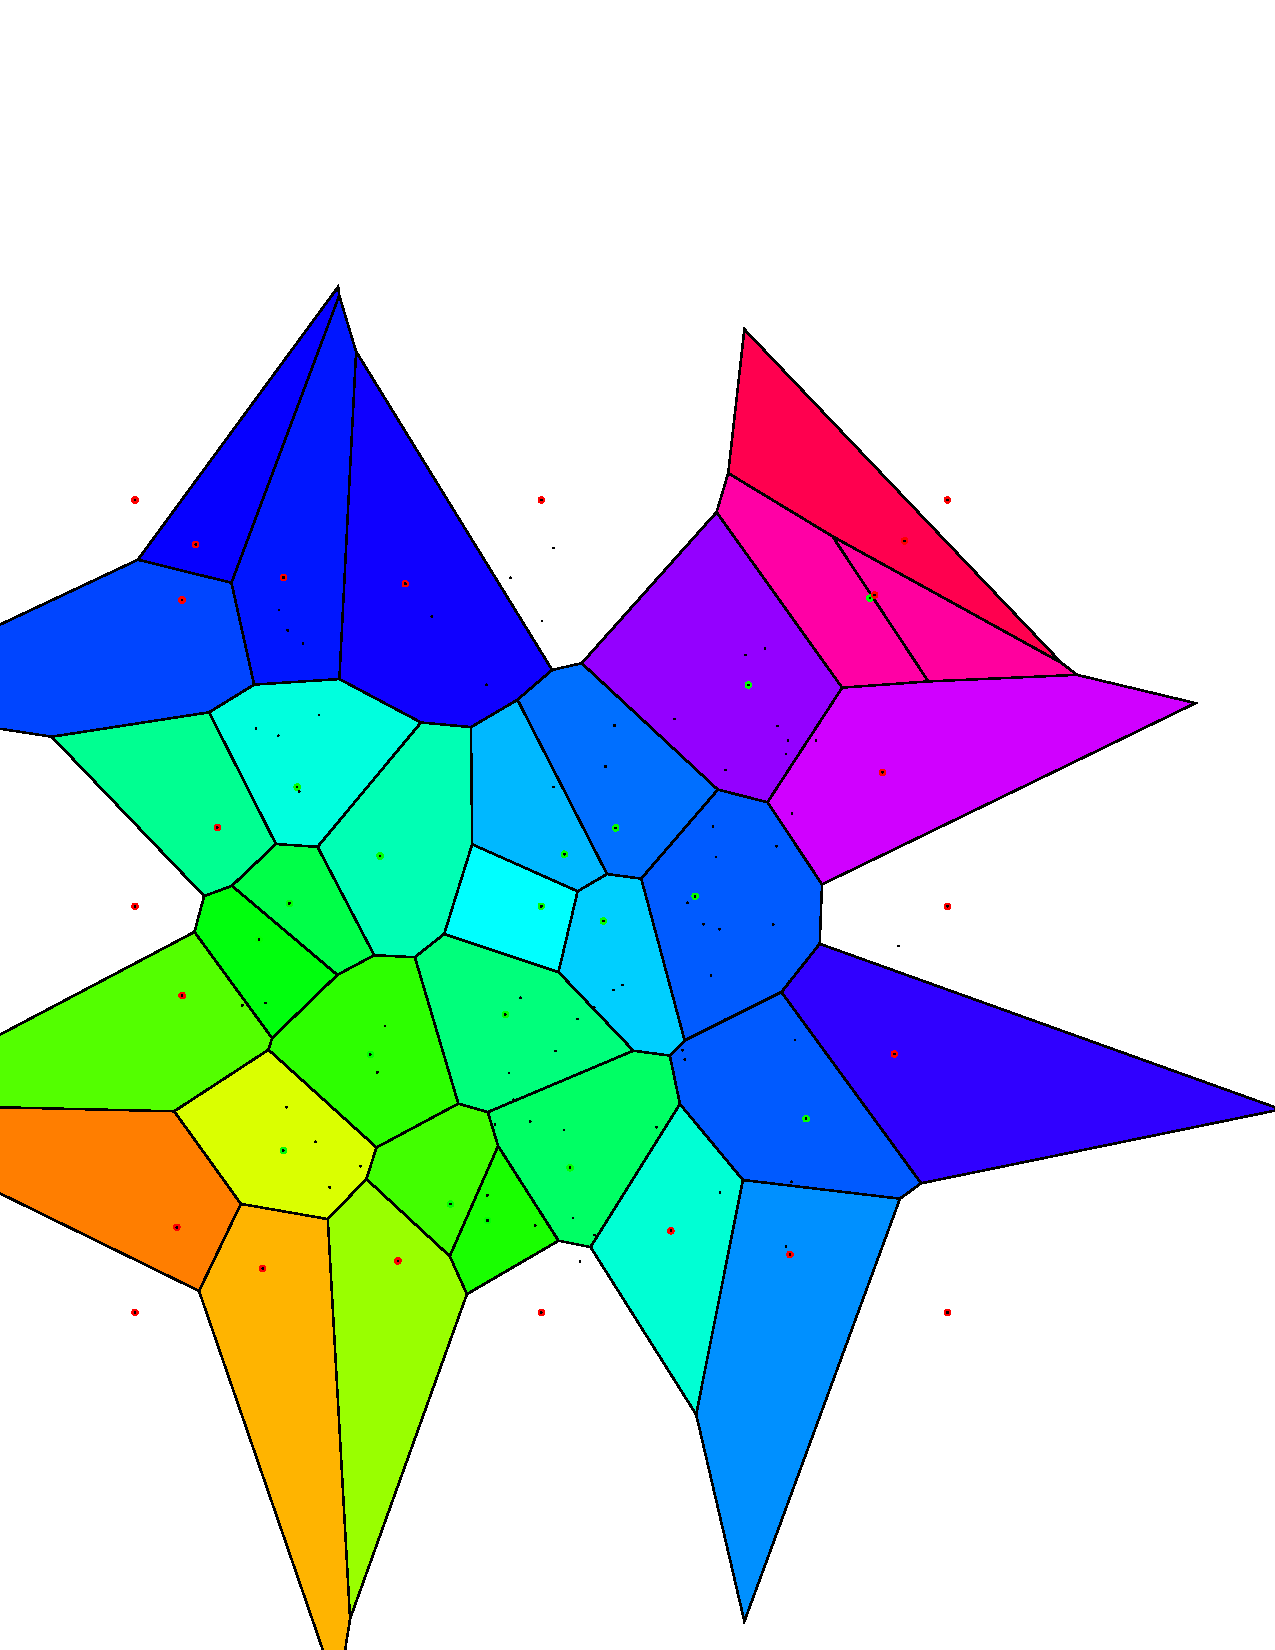
\includegraphics[trim={0 0 0 4cm},clip, width=0.45\textwidth]{../viz/100/voro17.pdf}}
   \subfloat {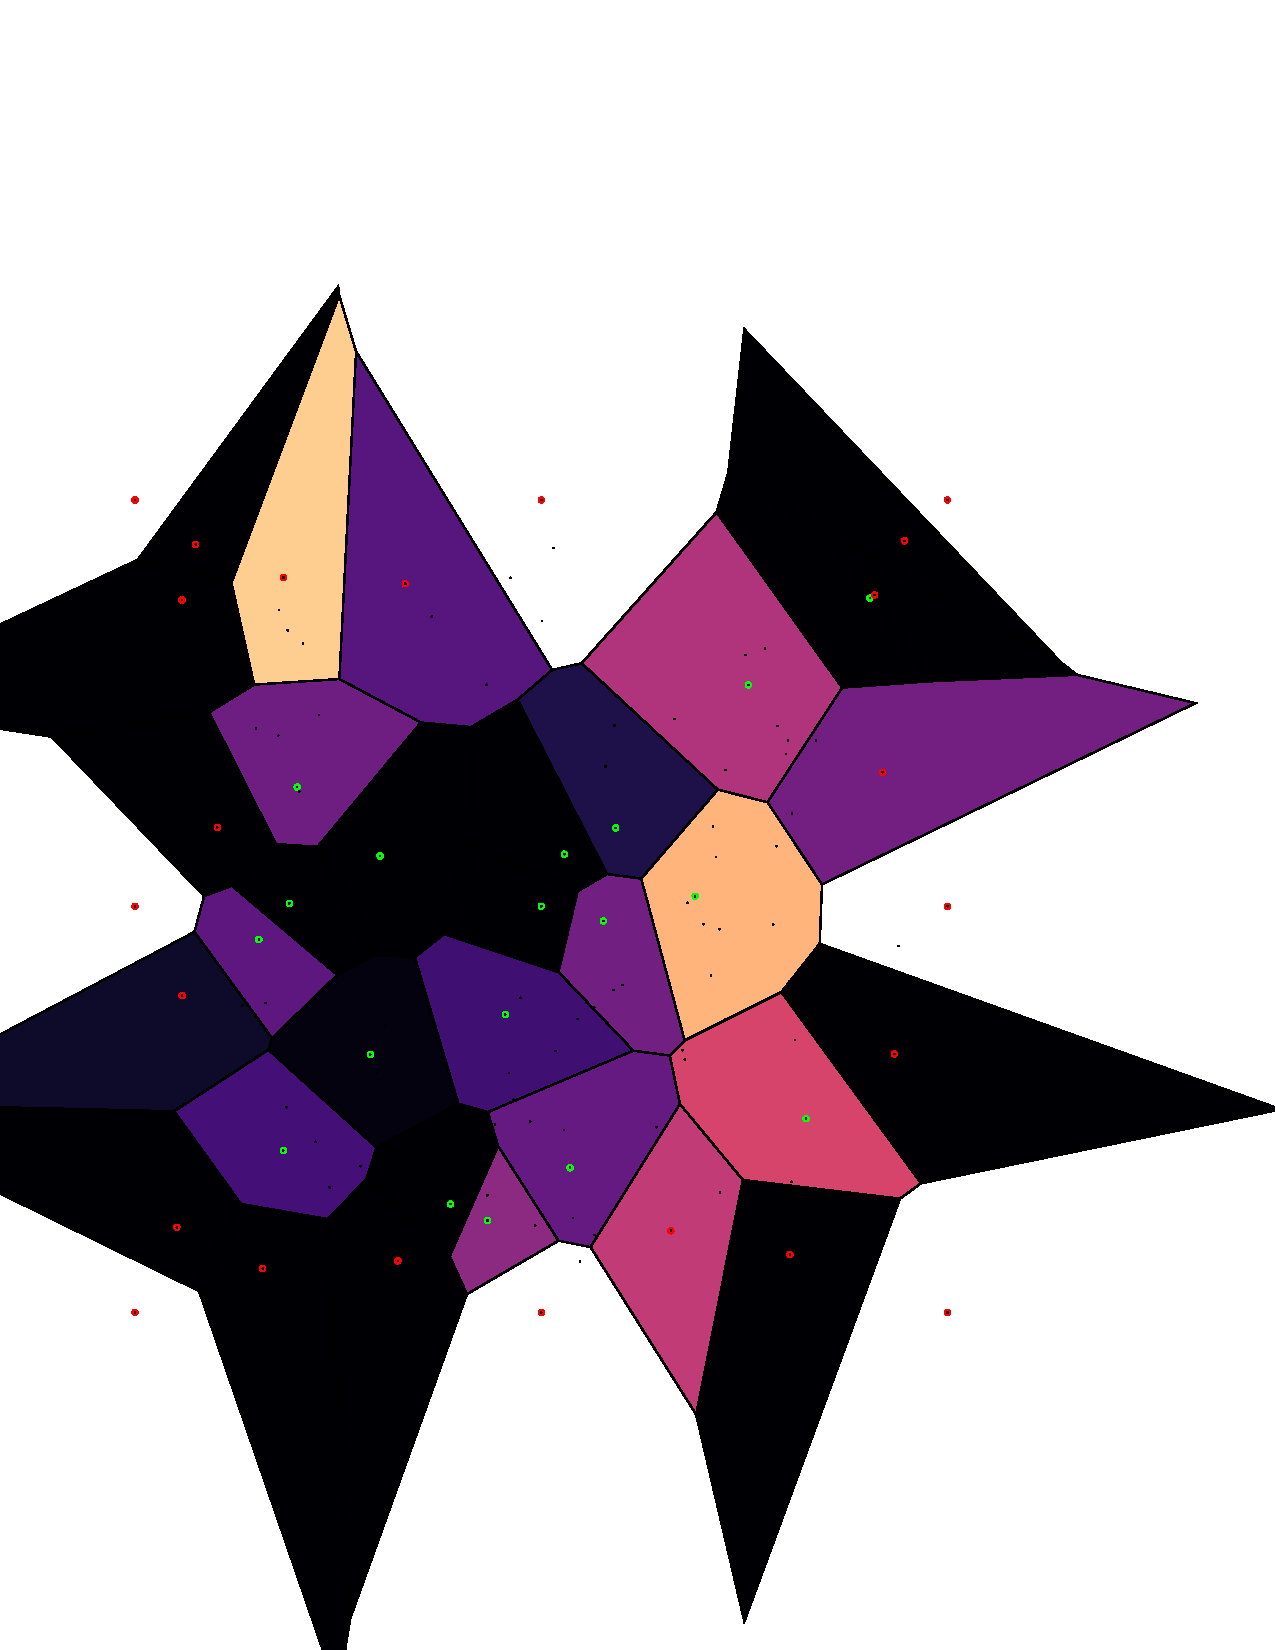
\includegraphics[trim={0 0 0 4cm},clip, width=0.45\textwidth]{../viz/100/voro_err17.pdf}}
\end{figure}
%======================================================

\newpage
\begin{figure}[!tbh]
\centering           
   \subfloat {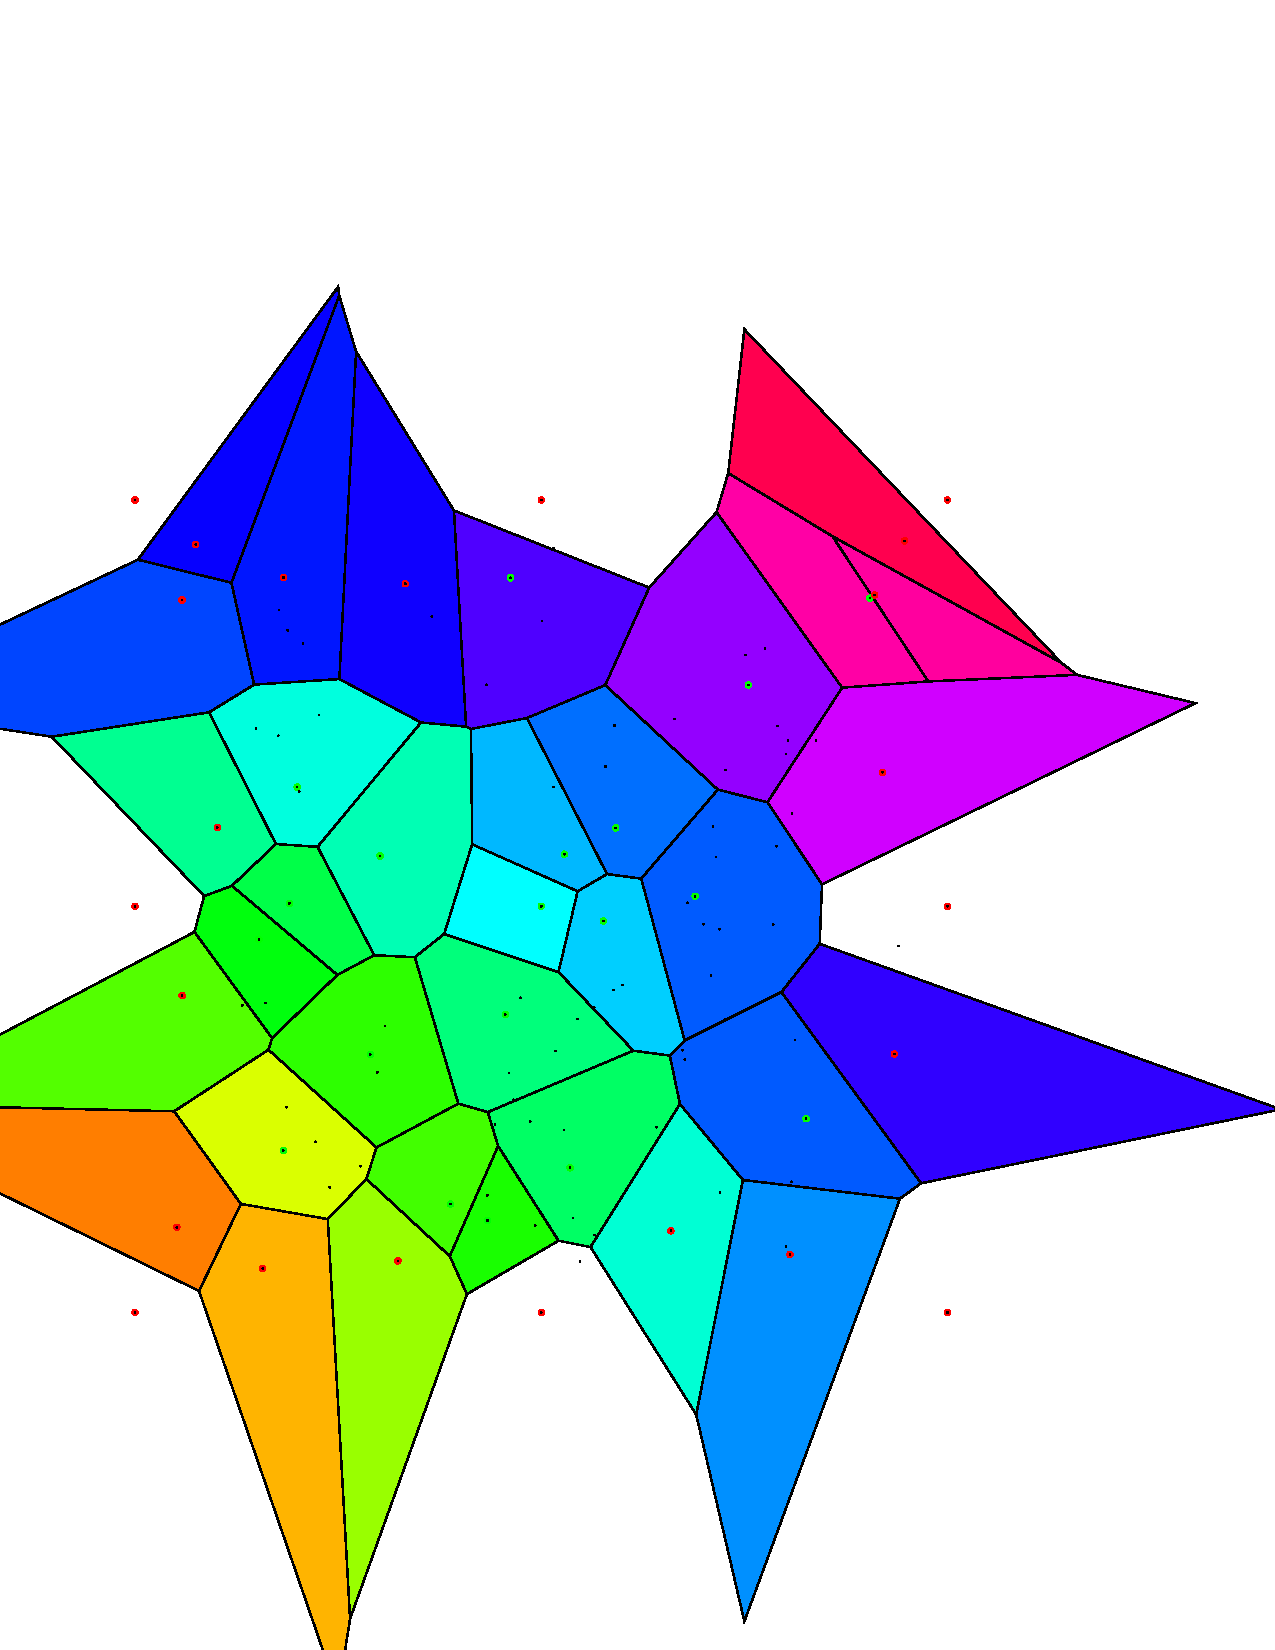
\includegraphics[trim={0 0 0 4cm},clip, width=0.45\textwidth]{../viz/100/voro18.pdf}}
   \subfloat {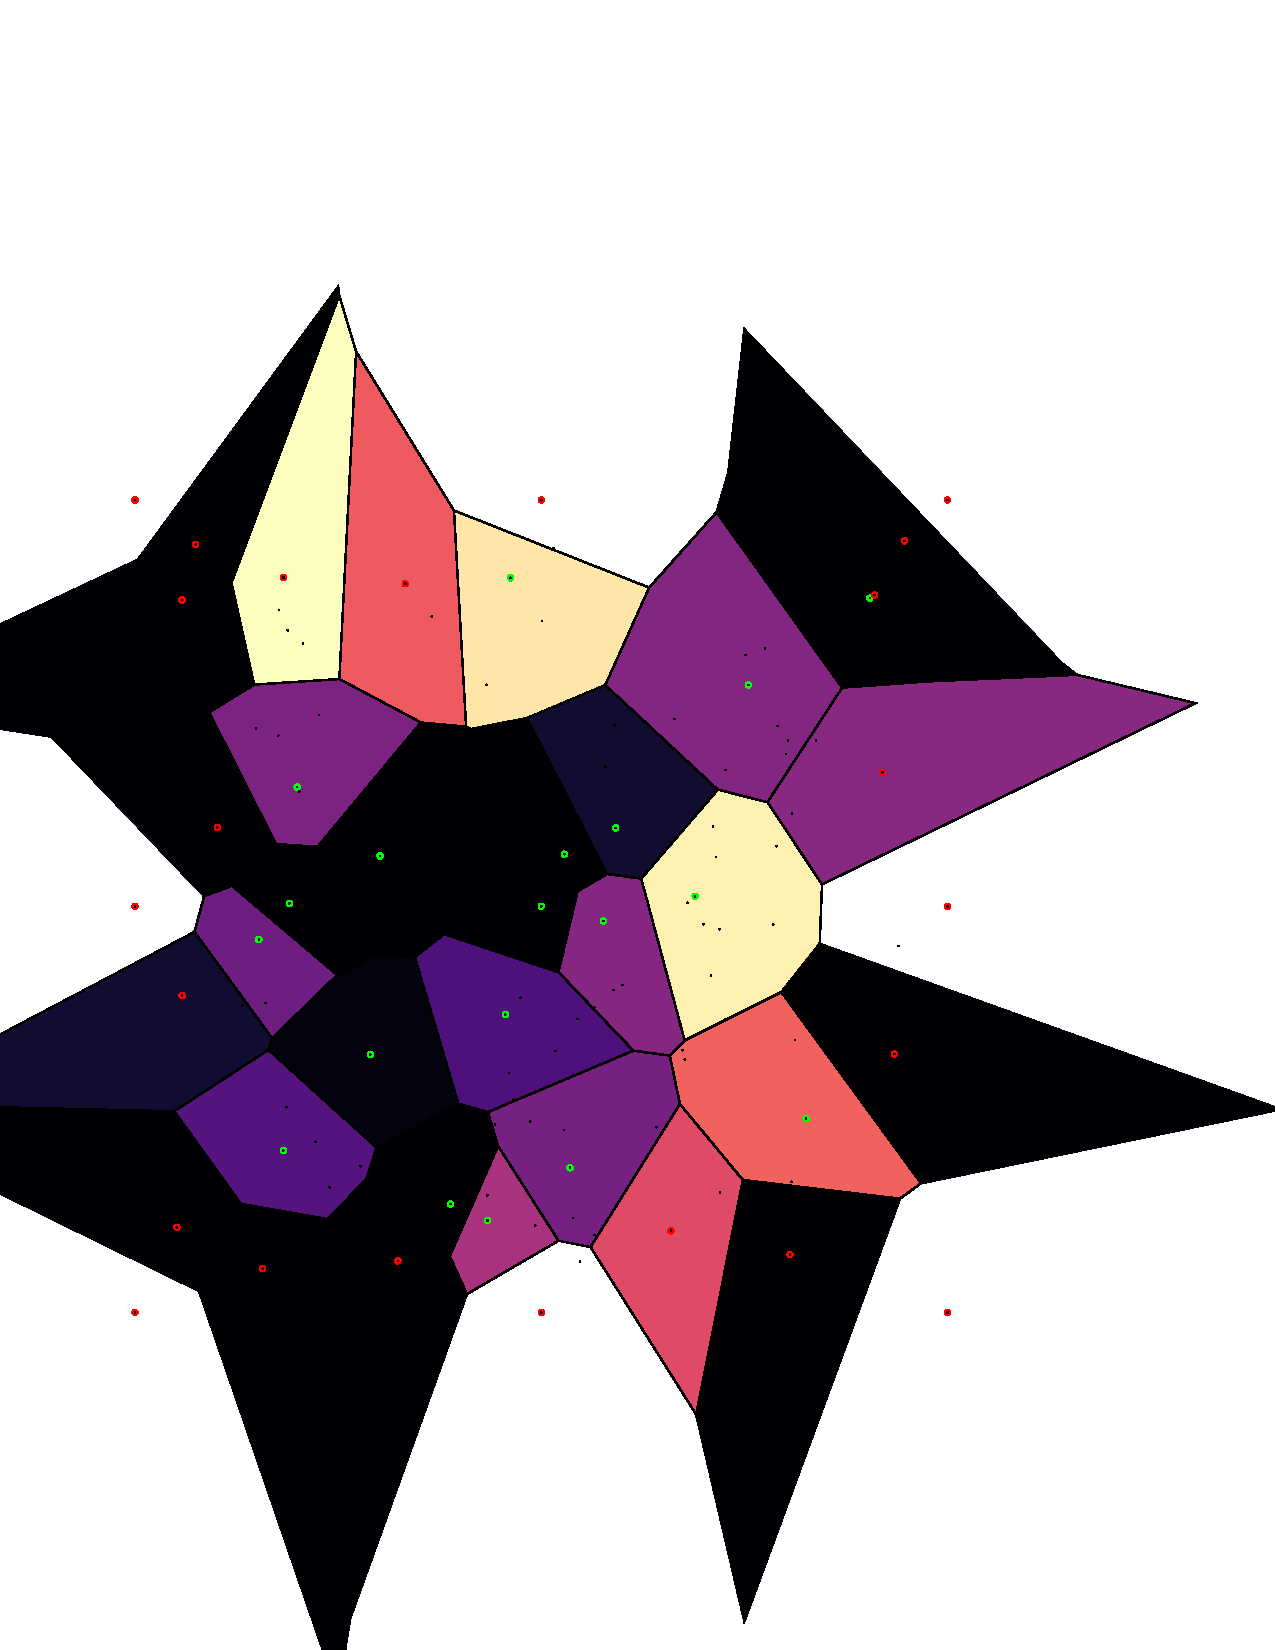
\includegraphics[trim={0 0 0 4cm},clip, width=0.45\textwidth]{../viz/100/voro_err18.pdf}}
   
   \subfloat {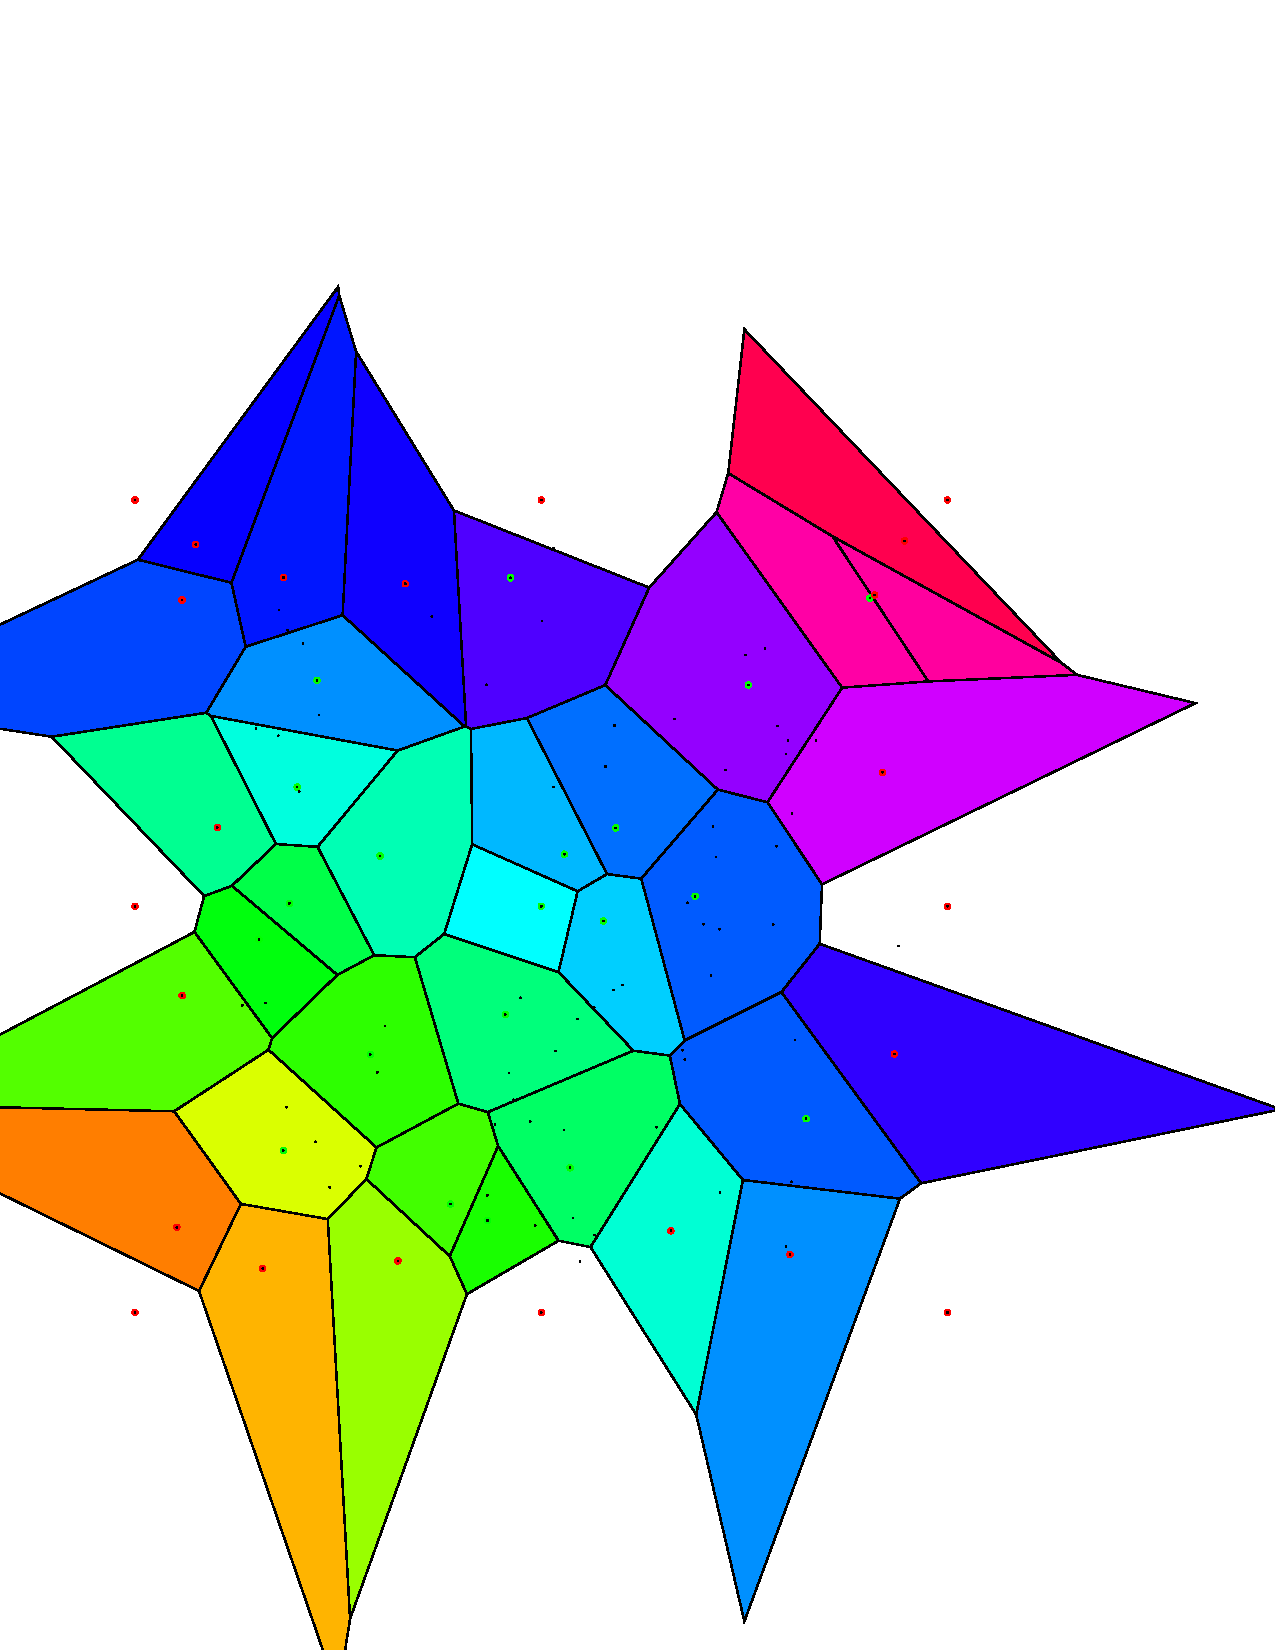
\includegraphics[trim={0 0 0 4cm},clip, width=0.45\textwidth]{../viz/100/voro19.pdf}}
   \subfloat {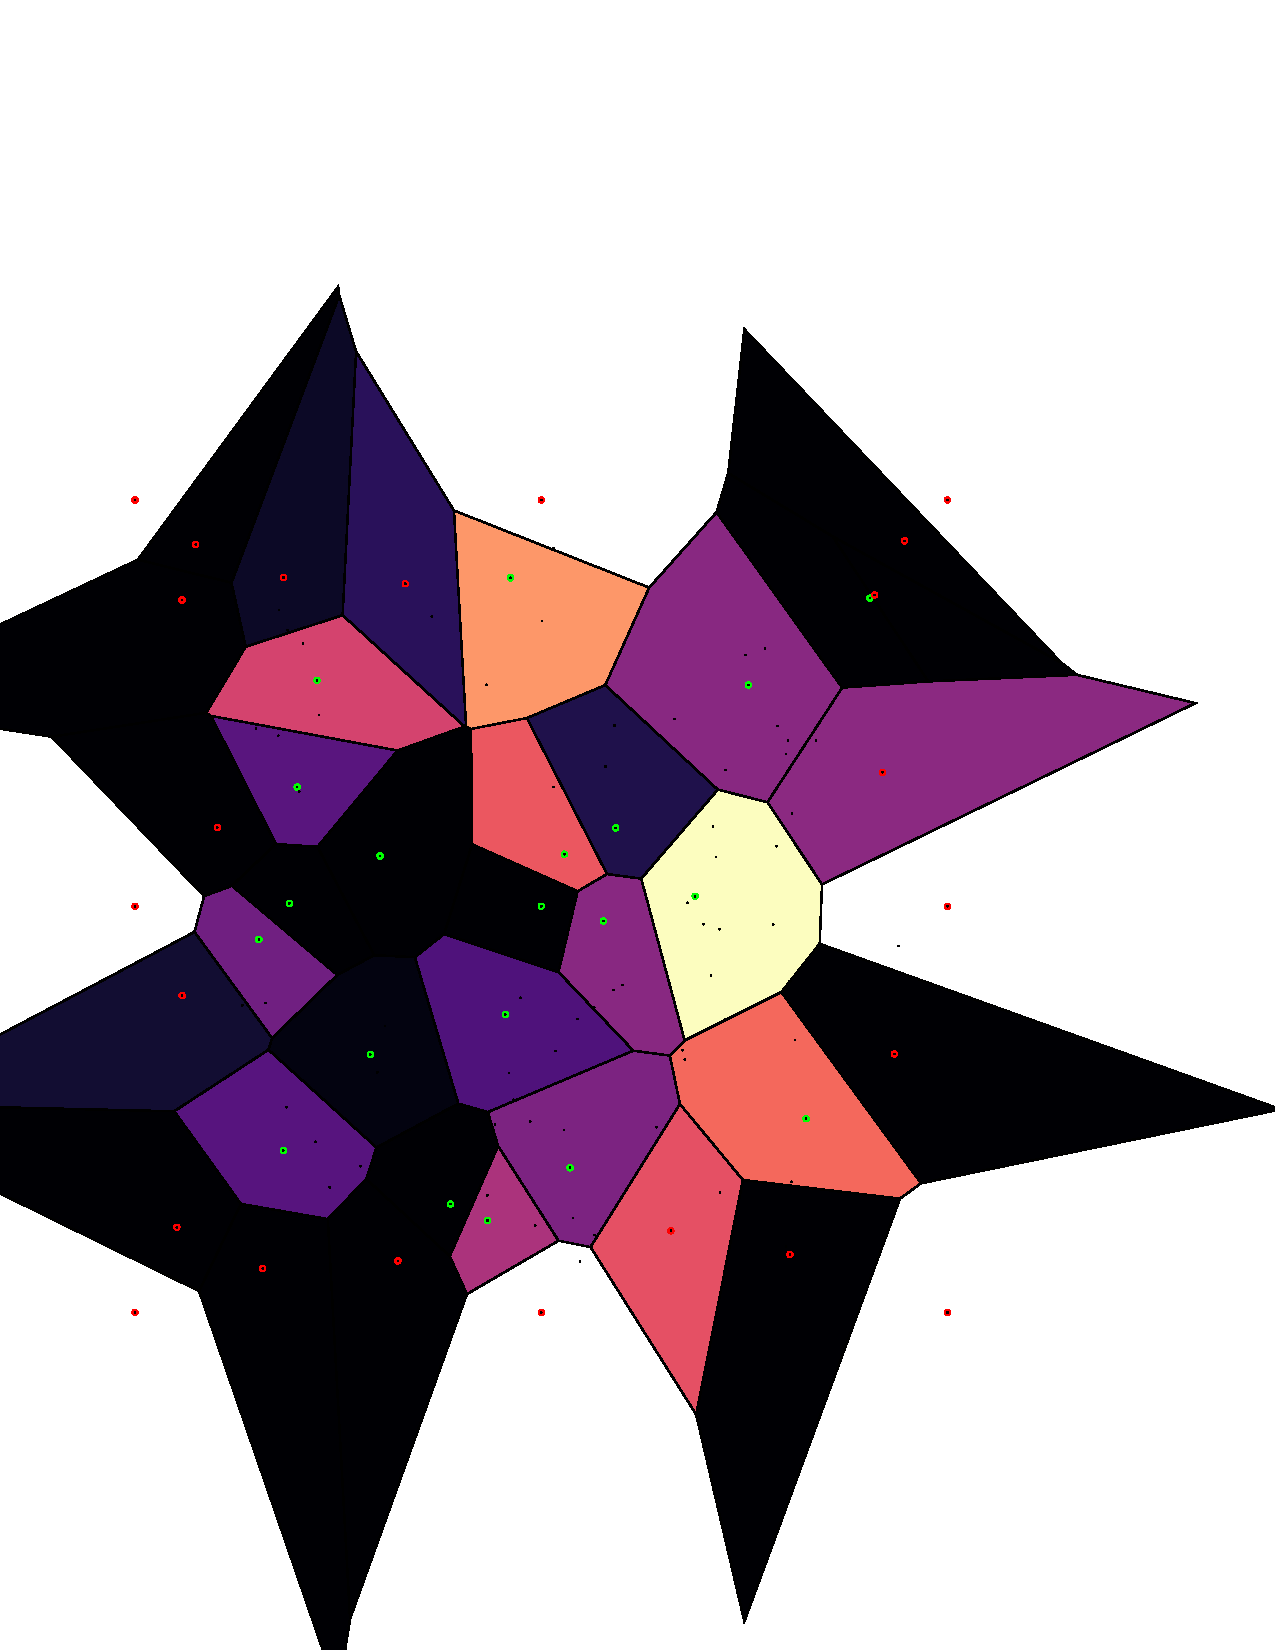
\includegraphics[trim={0 0 0 4cm},clip, width=0.45\textwidth]{../viz/100/voro_err19.pdf}}
\end{figure}
%======================================================


\newpage
\begin{figure}[!tbh]
\centering           
   \subfloat {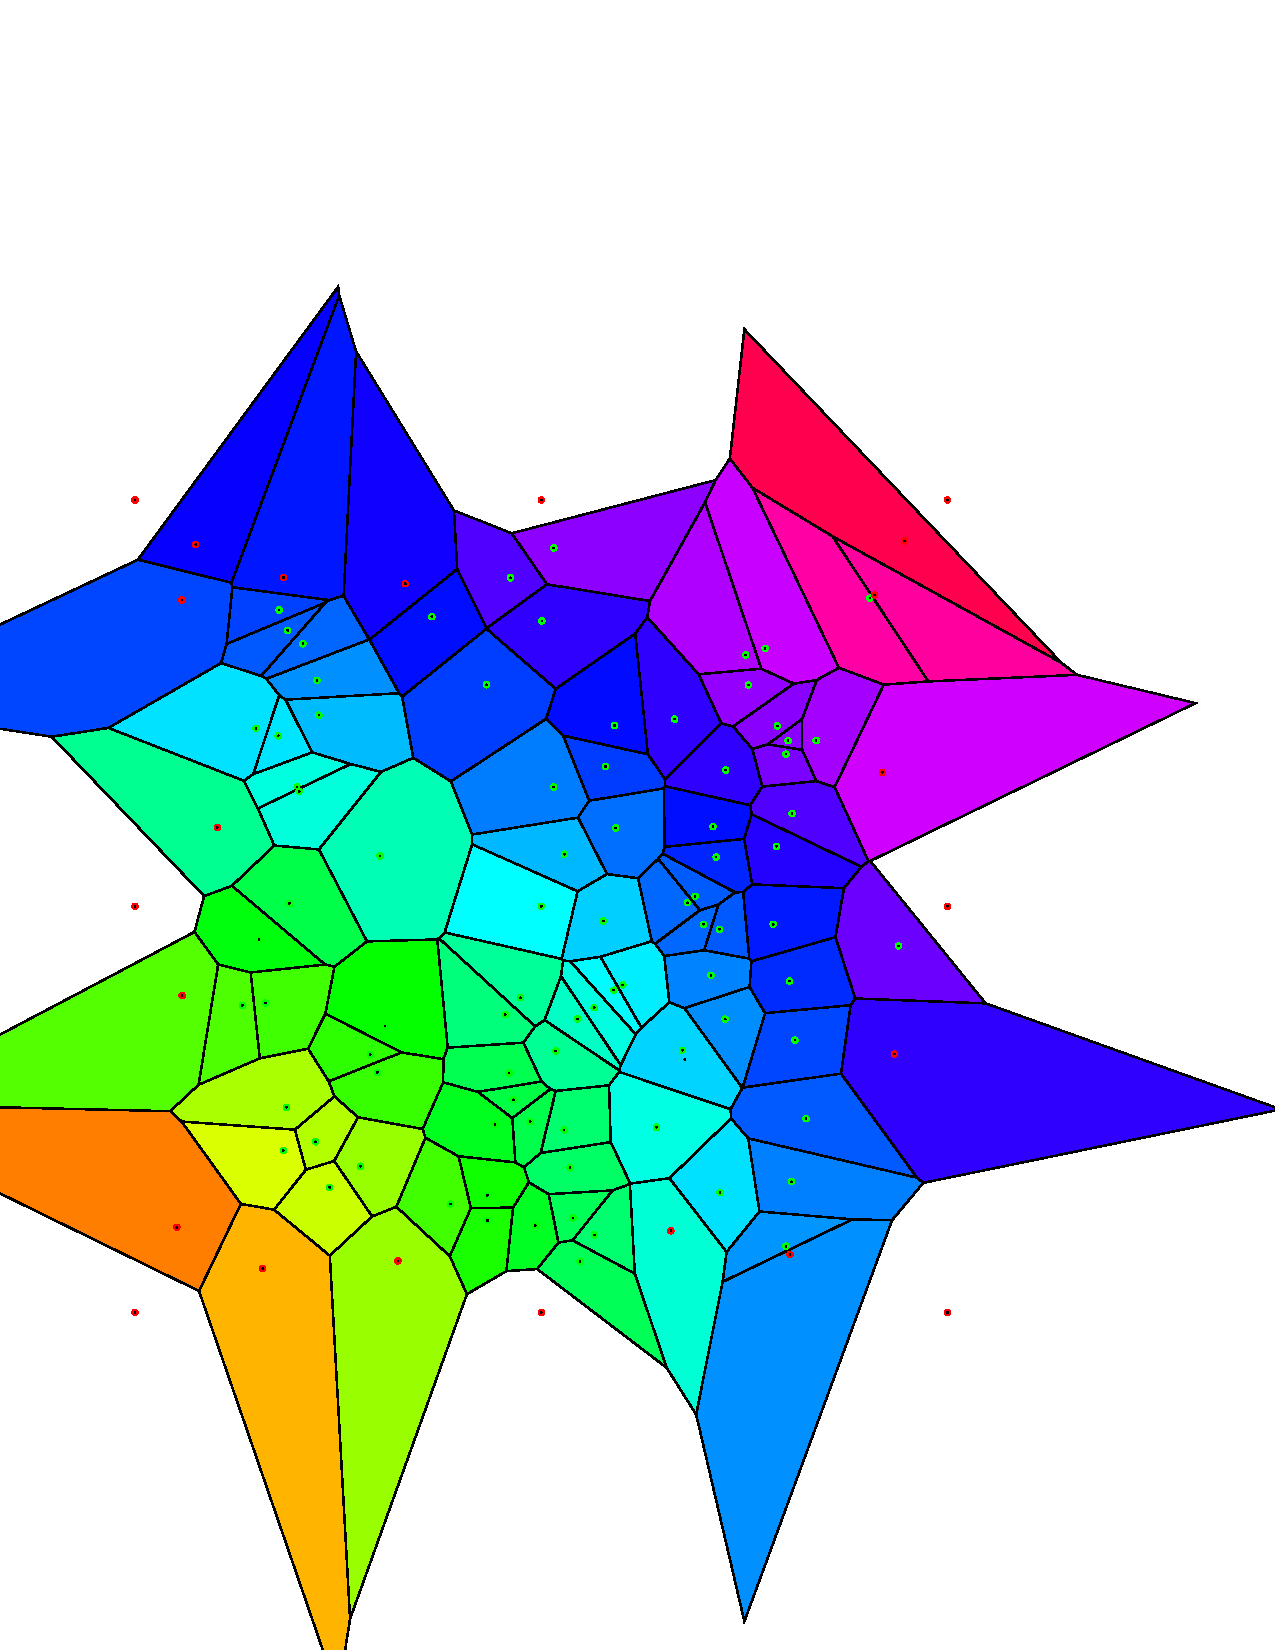
\includegraphics[trim={0 0 0 4cm},clip, width=0.45\textwidth]{../viz/100/voro83.pdf}}
   \subfloat {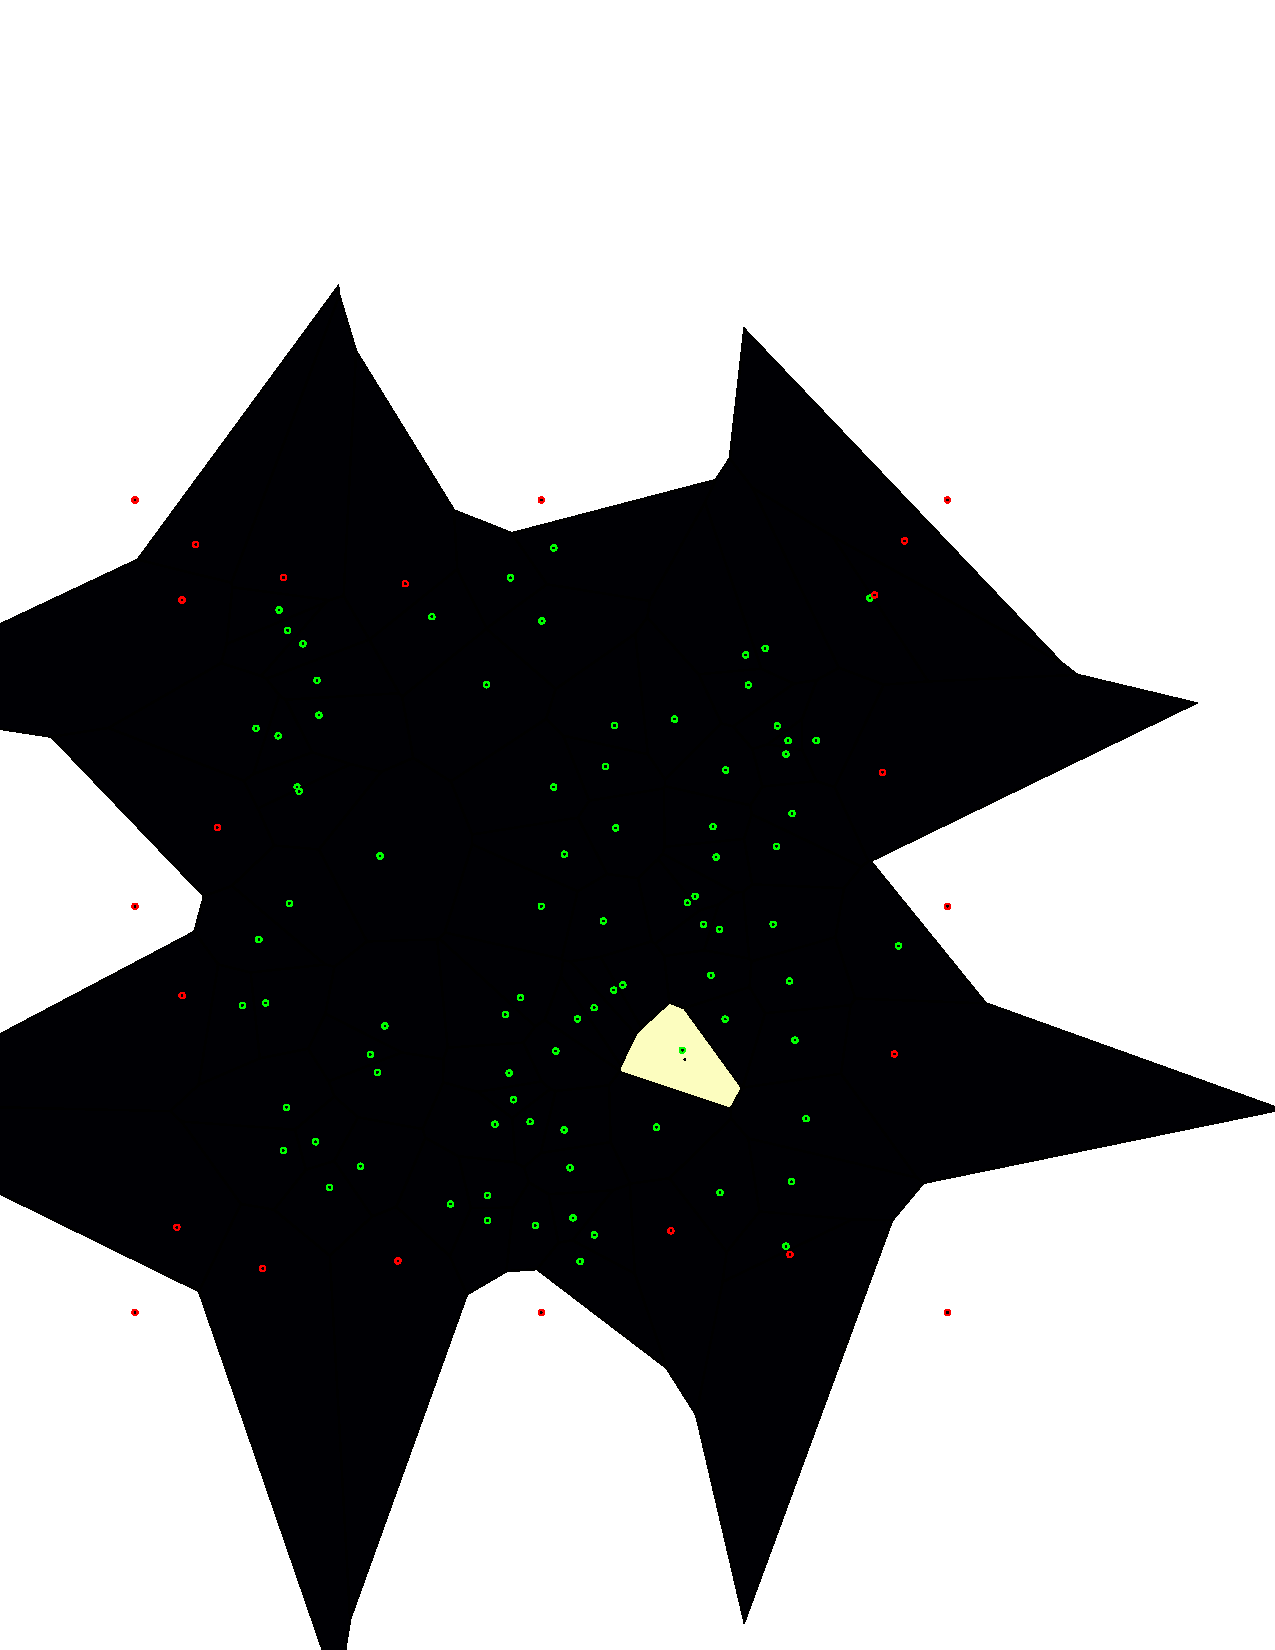
\includegraphics[trim={0 0 0 4cm},clip, width=0.45\textwidth]{../viz/100/voro_err83.pdf}}
   
   \subfloat [Final] {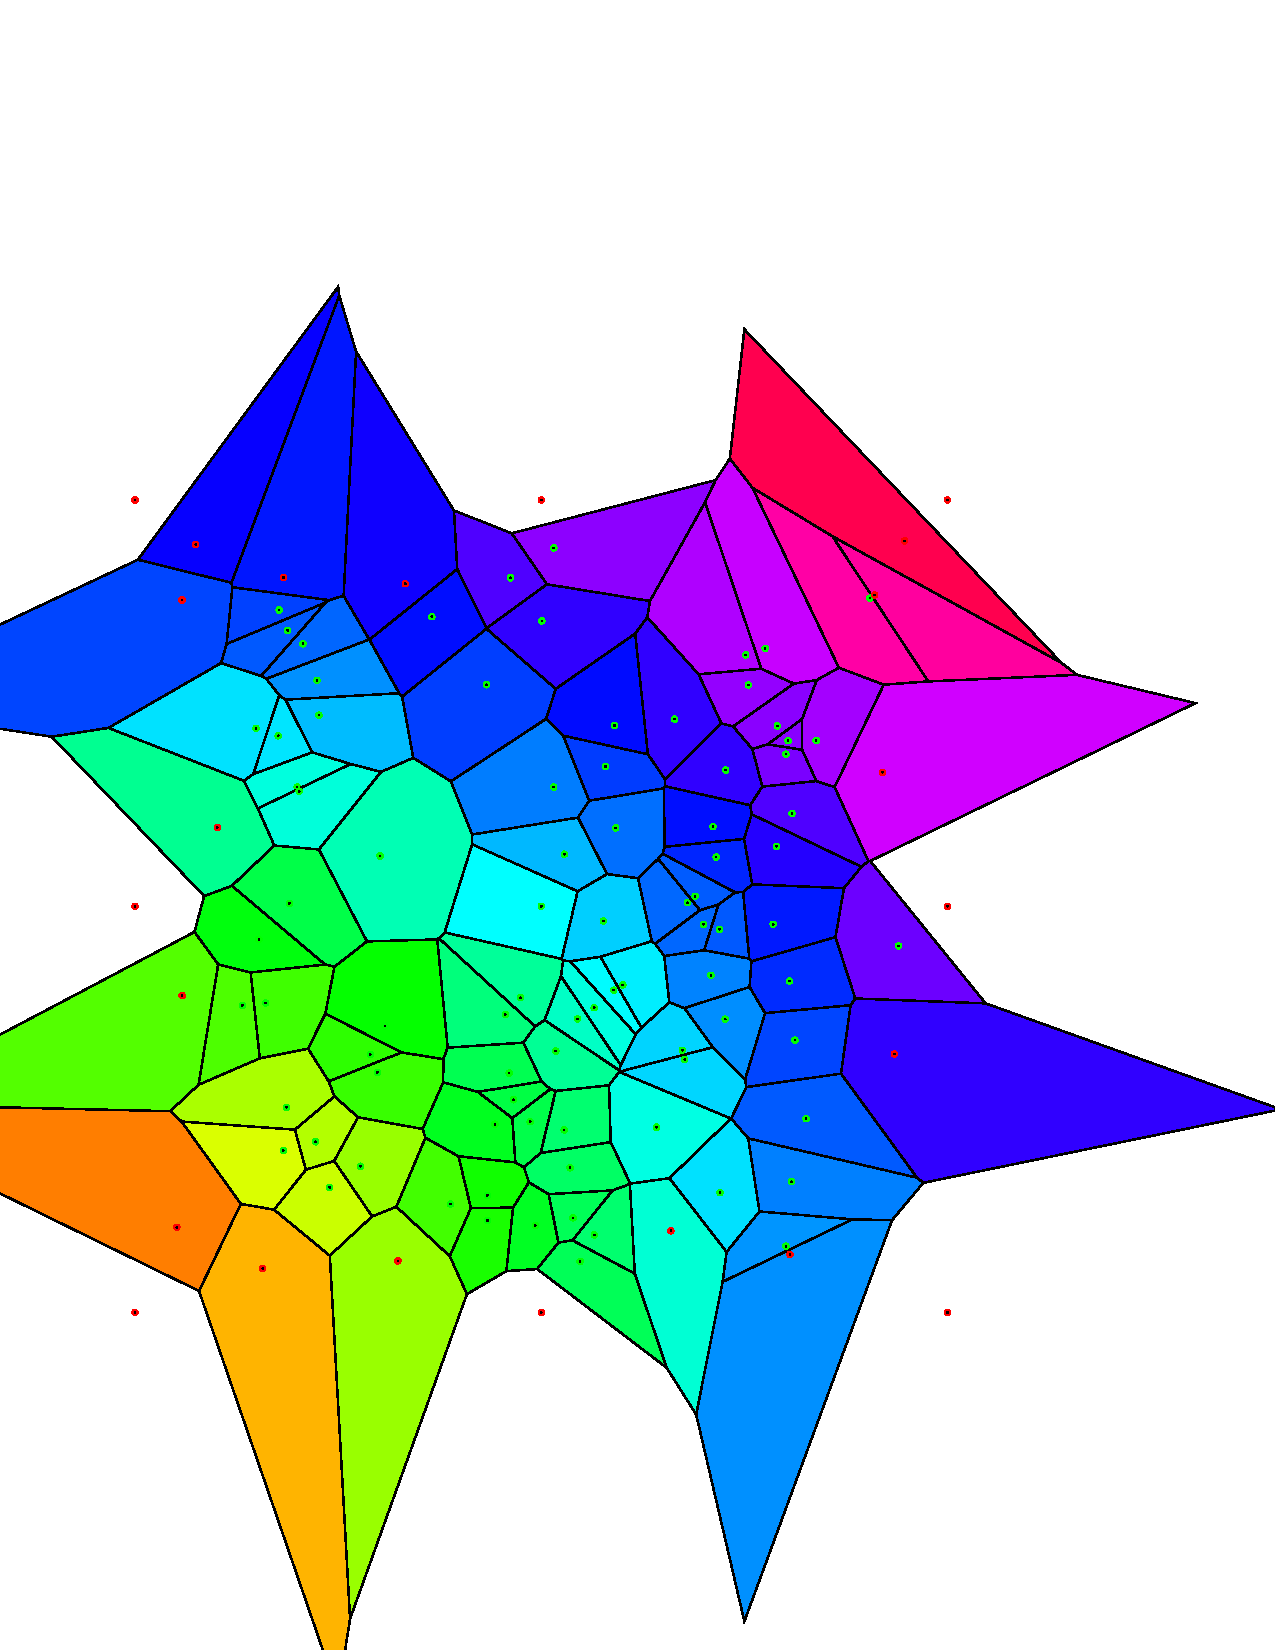
\includegraphics[trim={0 0 0 4cm},clip, width=0.45\textwidth]{../viz/100/voro84.pdf}}
\end{figure}
%======================================================

\newpage
The following is a snapshots of the insertion process after each 100 point being inserted in a 508 original data points. 



\newpage
\begin{figure}[!tbh]
\centering           
   \subfloat [A] {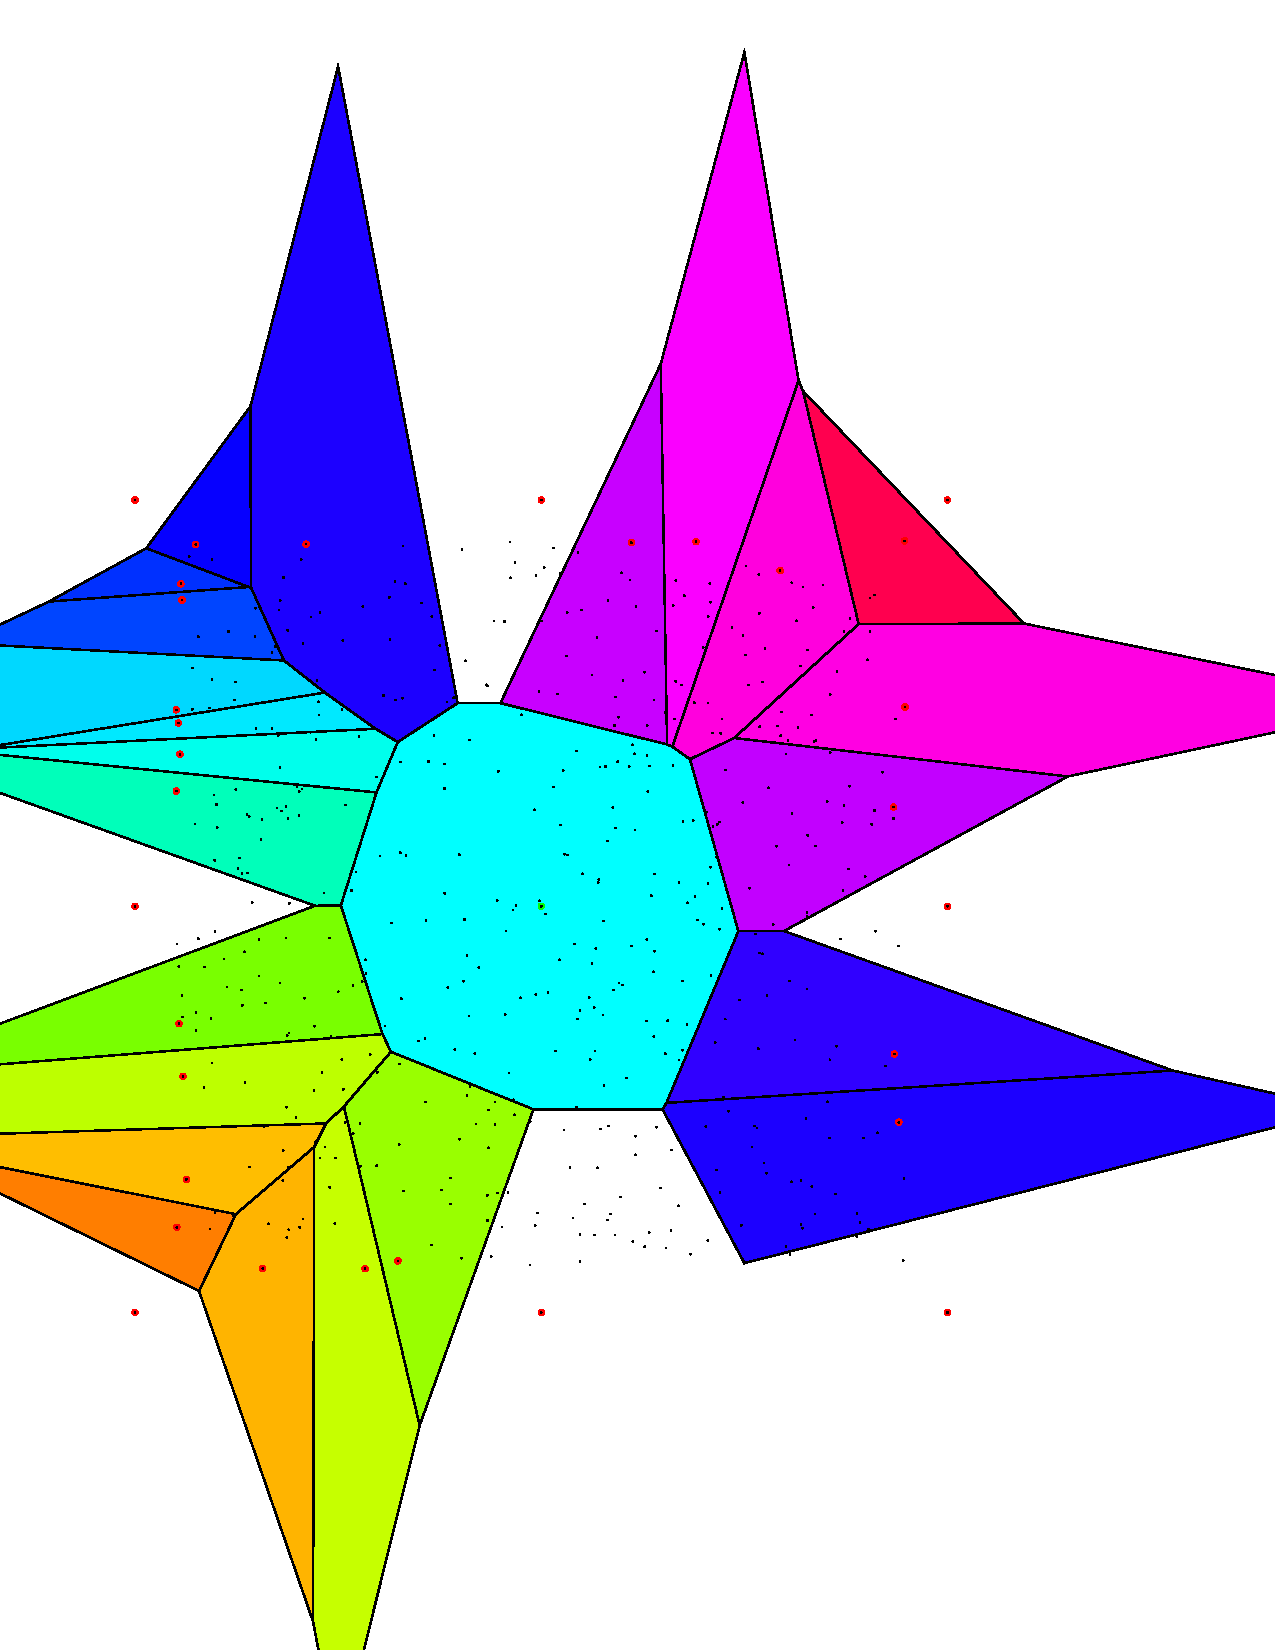
\includegraphics[trim={0 0 0 2cm},clip, width=0.33\textwidth]{../viz/500/voro0.pdf}}
   \subfloat [B] {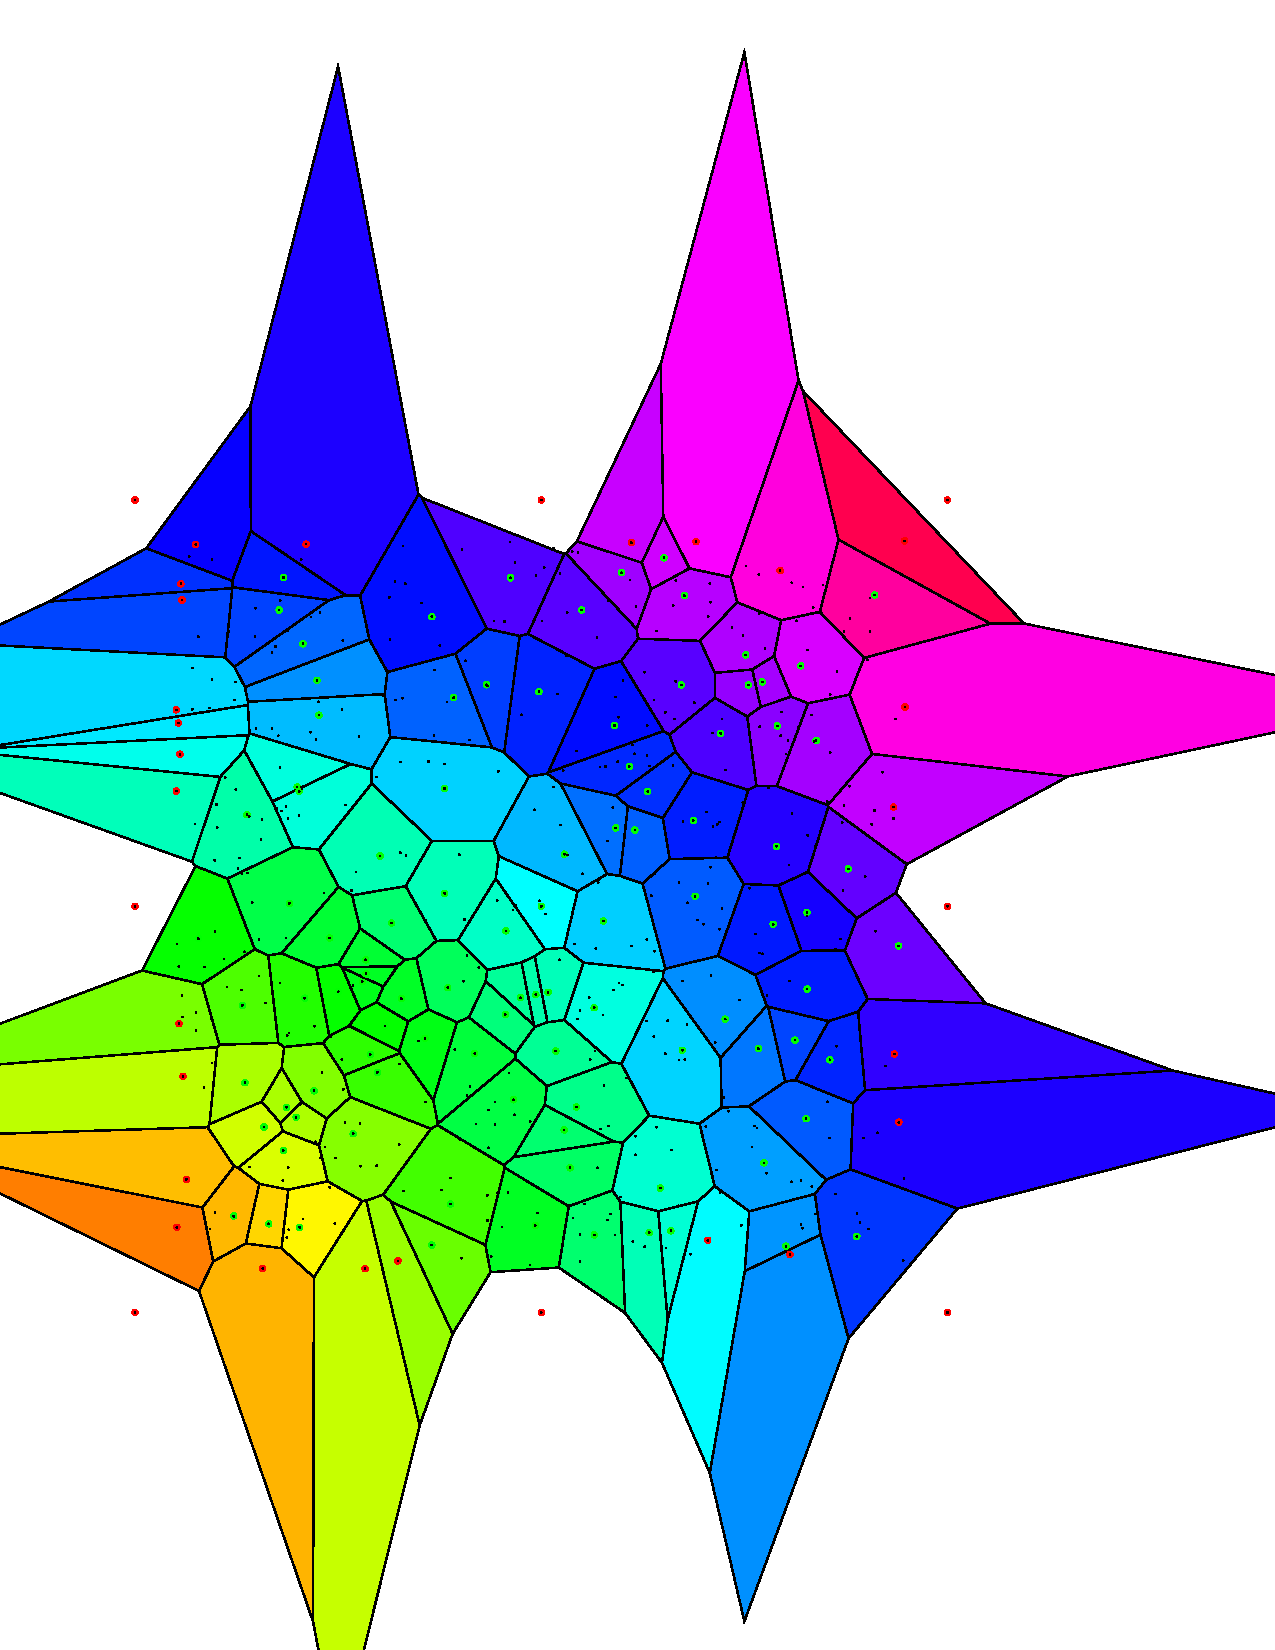
\includegraphics[trim={0 0 0 2cm},clip, width=0.33\textwidth]{../viz/500/voro100.pdf}}
   \subfloat [C] {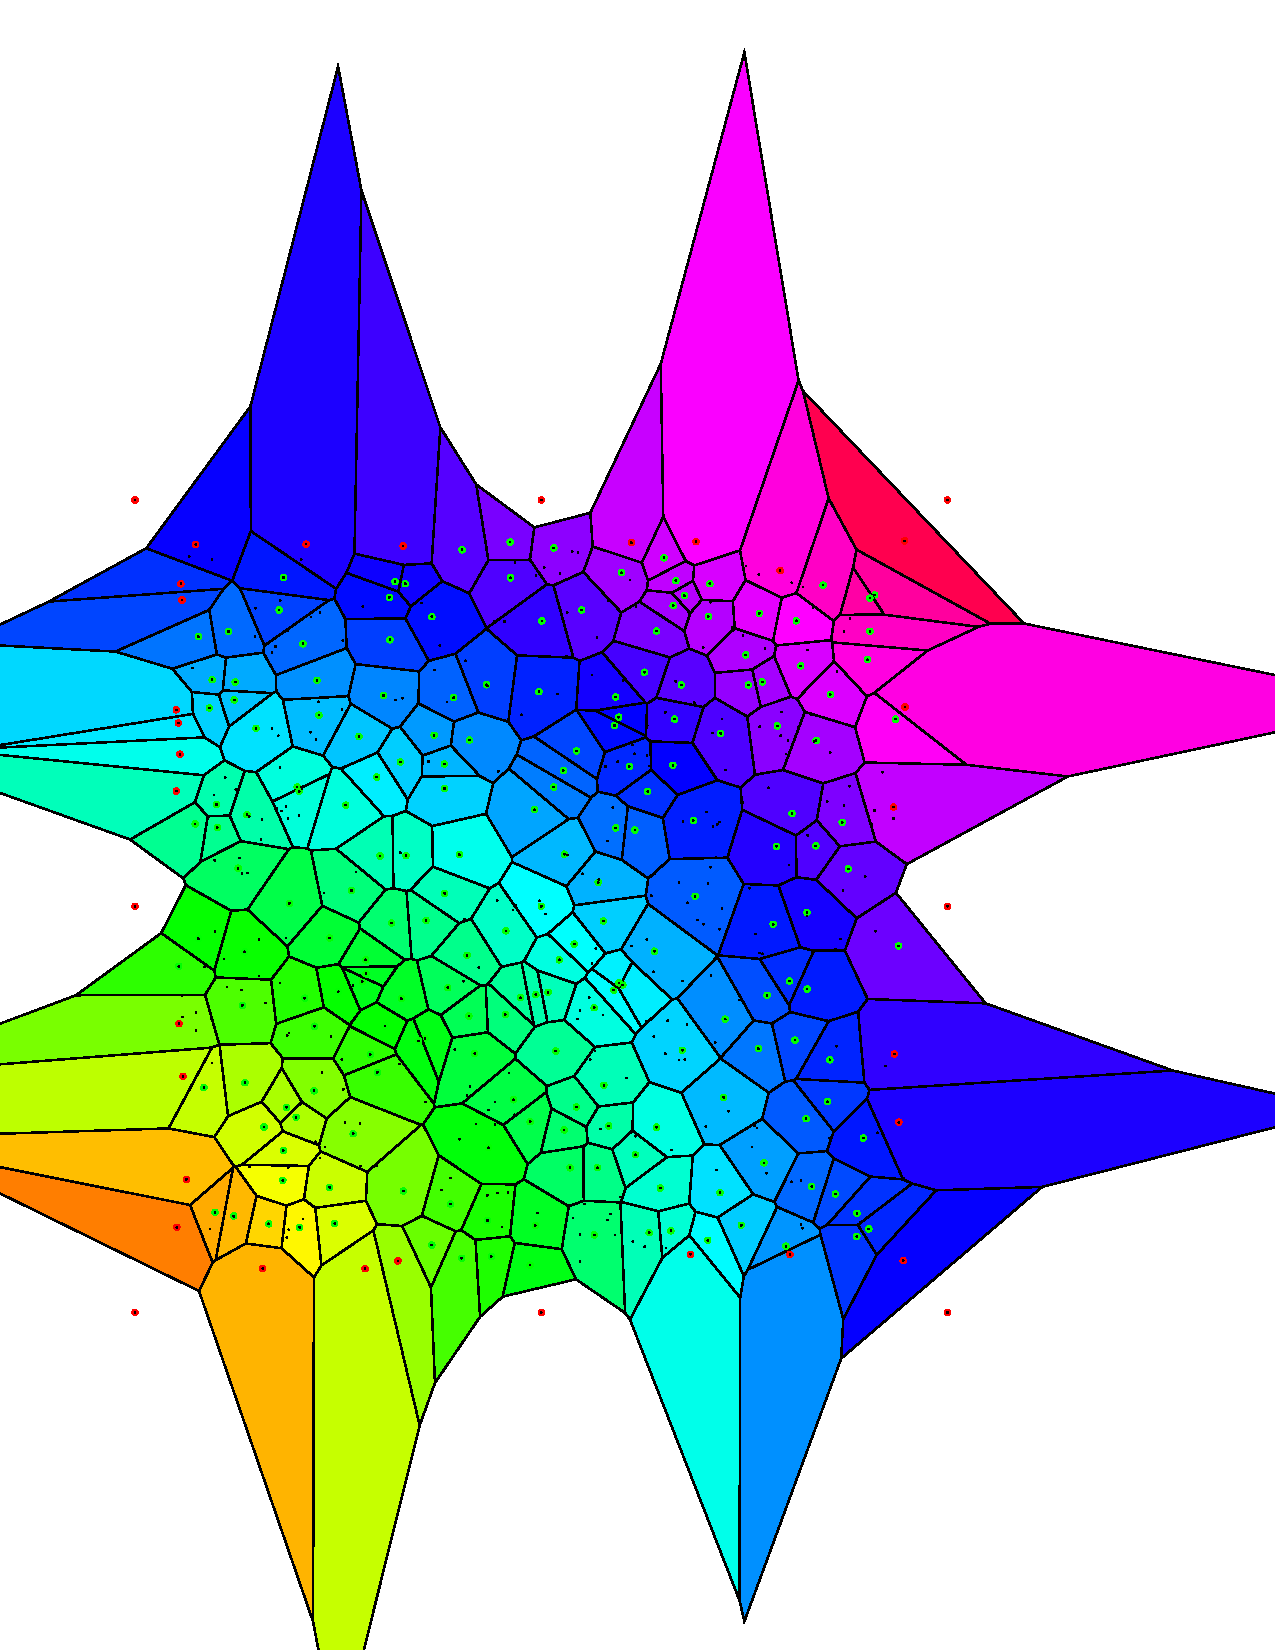
\includegraphics[trim={0 0 0 2cm},clip, width=0.33\textwidth]{../viz/500/voro200.pdf}}
   
   \subfloat [D] {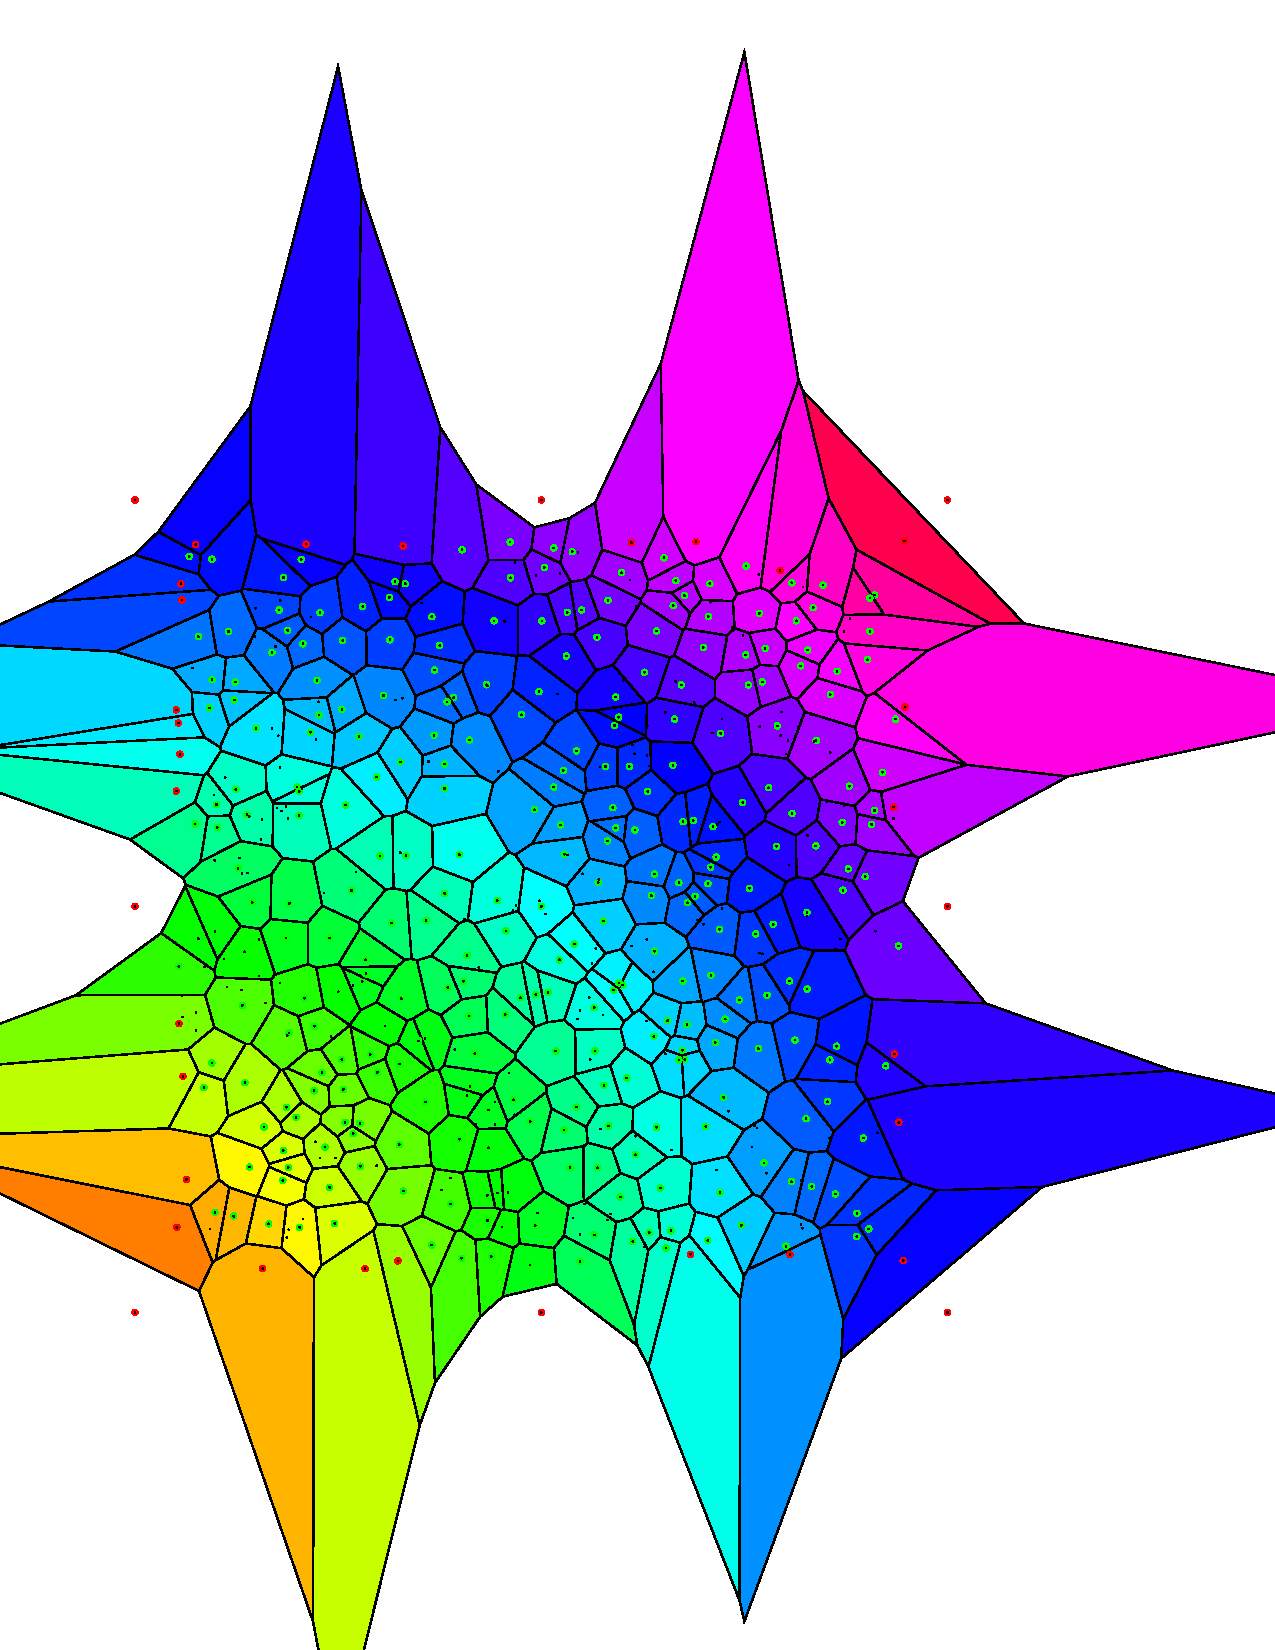
\includegraphics[trim={0 0 0 2cm},clip, width=0.33\textwidth]{../viz/500/voro300.pdf}}
   \subfloat [E] {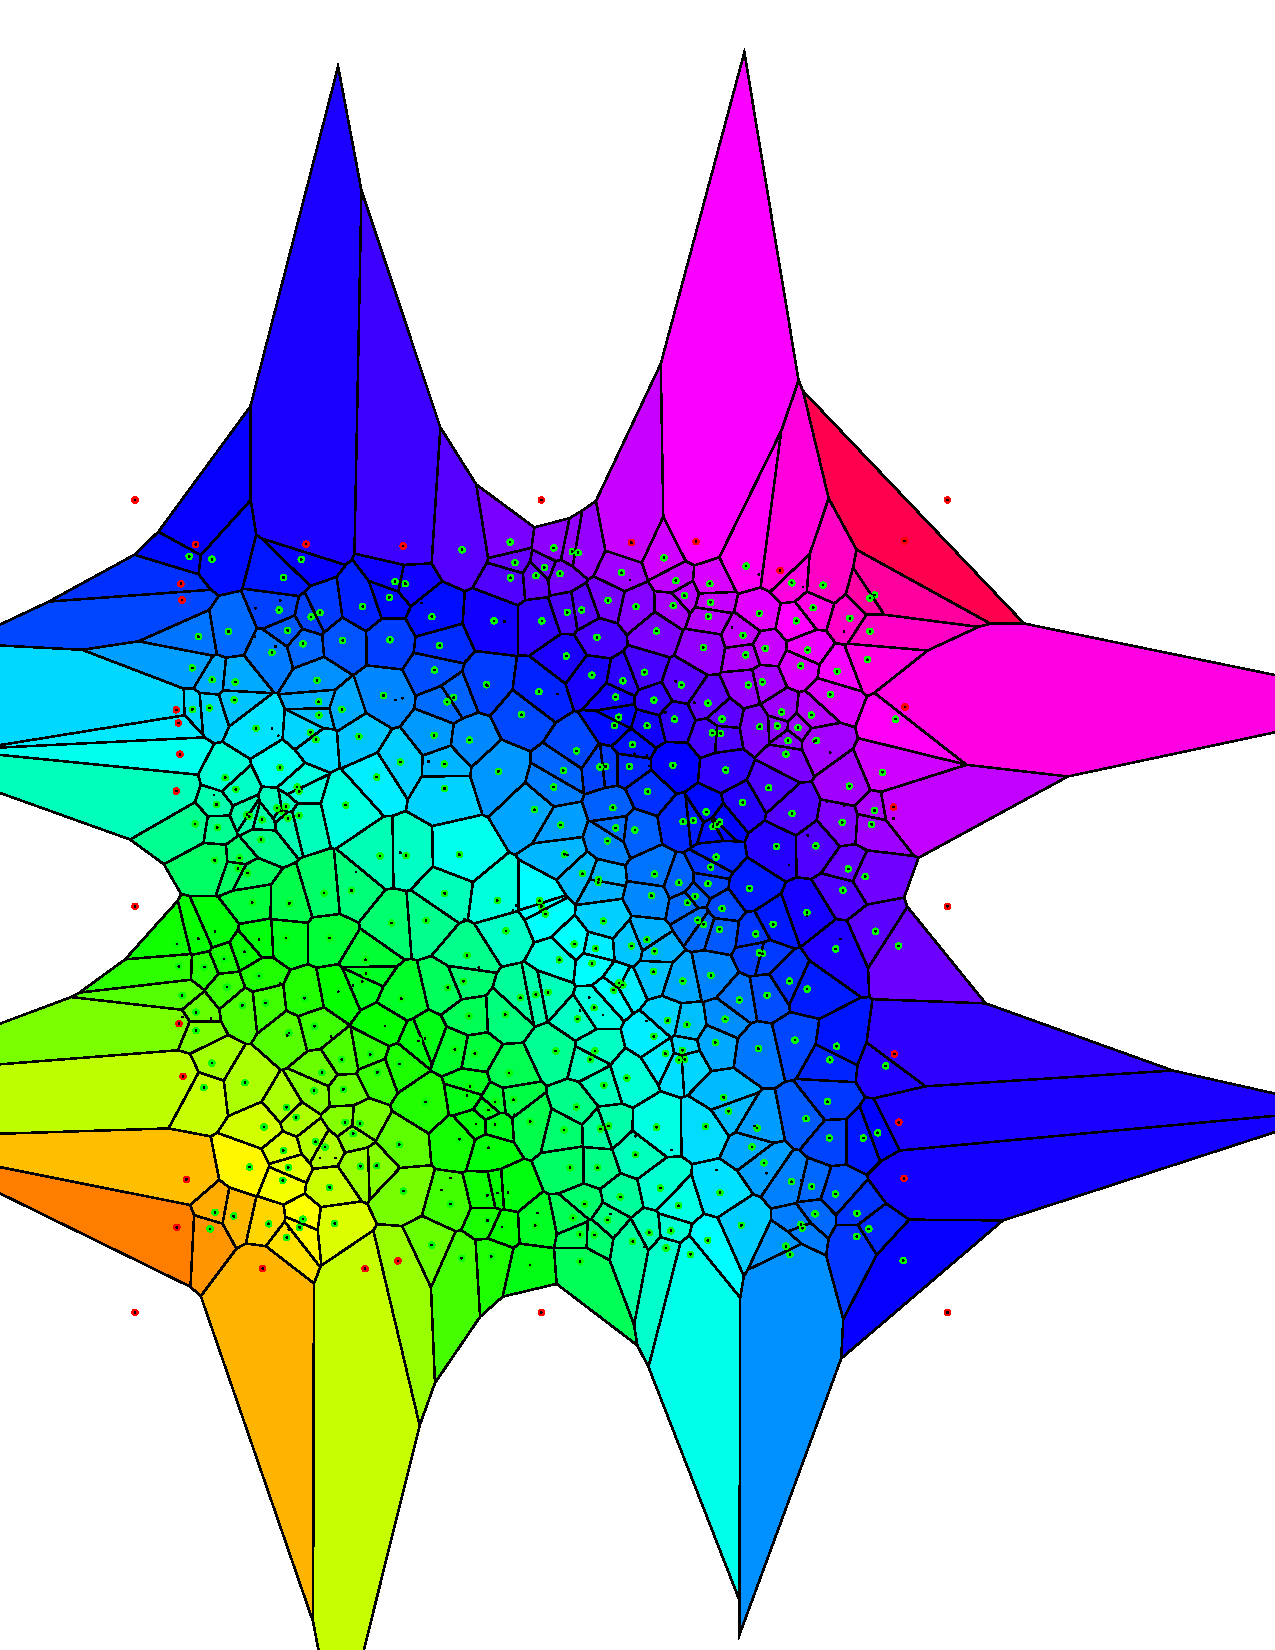
\includegraphics[trim={0 0 0 2cm},clip, width=0.33\textwidth]{../viz/500/voro400.pdf}}
   \subfloat [Final] {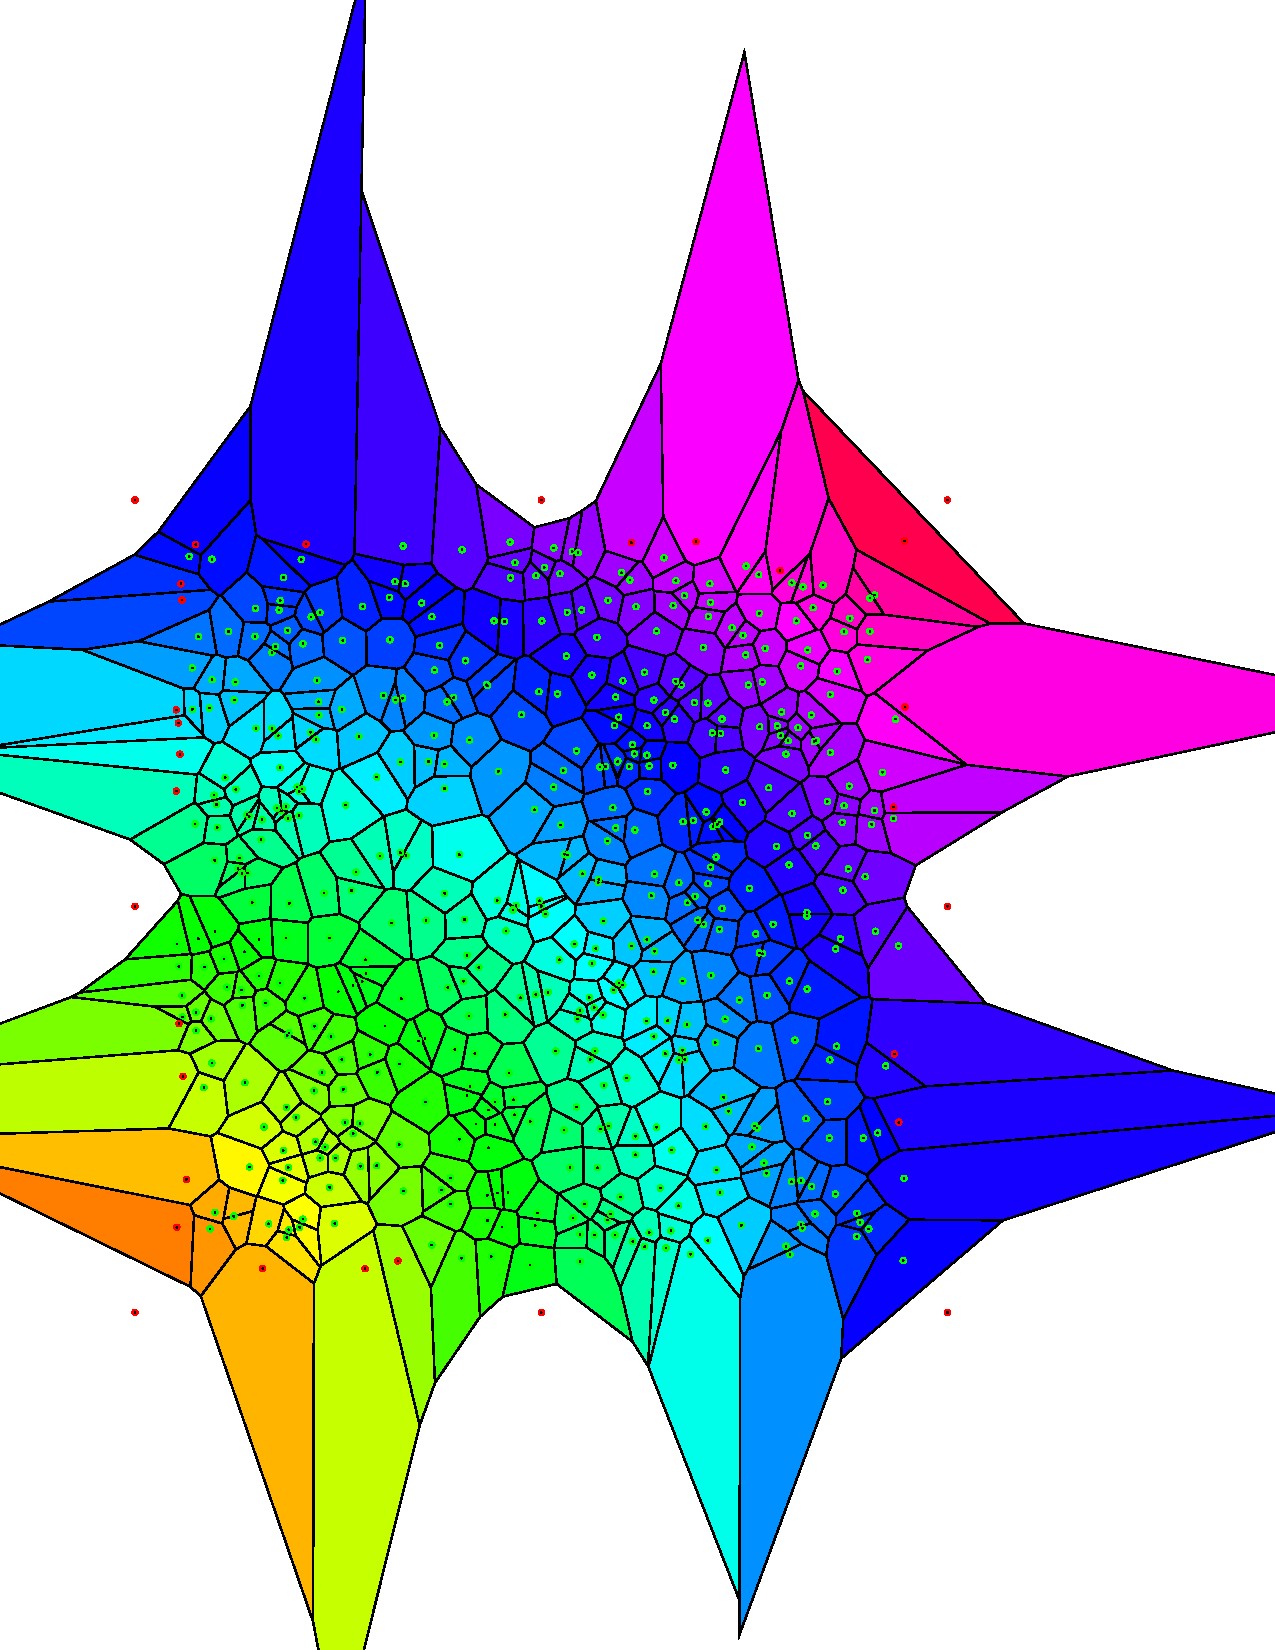
\includegraphics[trim={0 0 0 2cm},clip, width=0.33\textwidth]{../viz/500/voro476.pdf}}
   
   \subfloat [A] {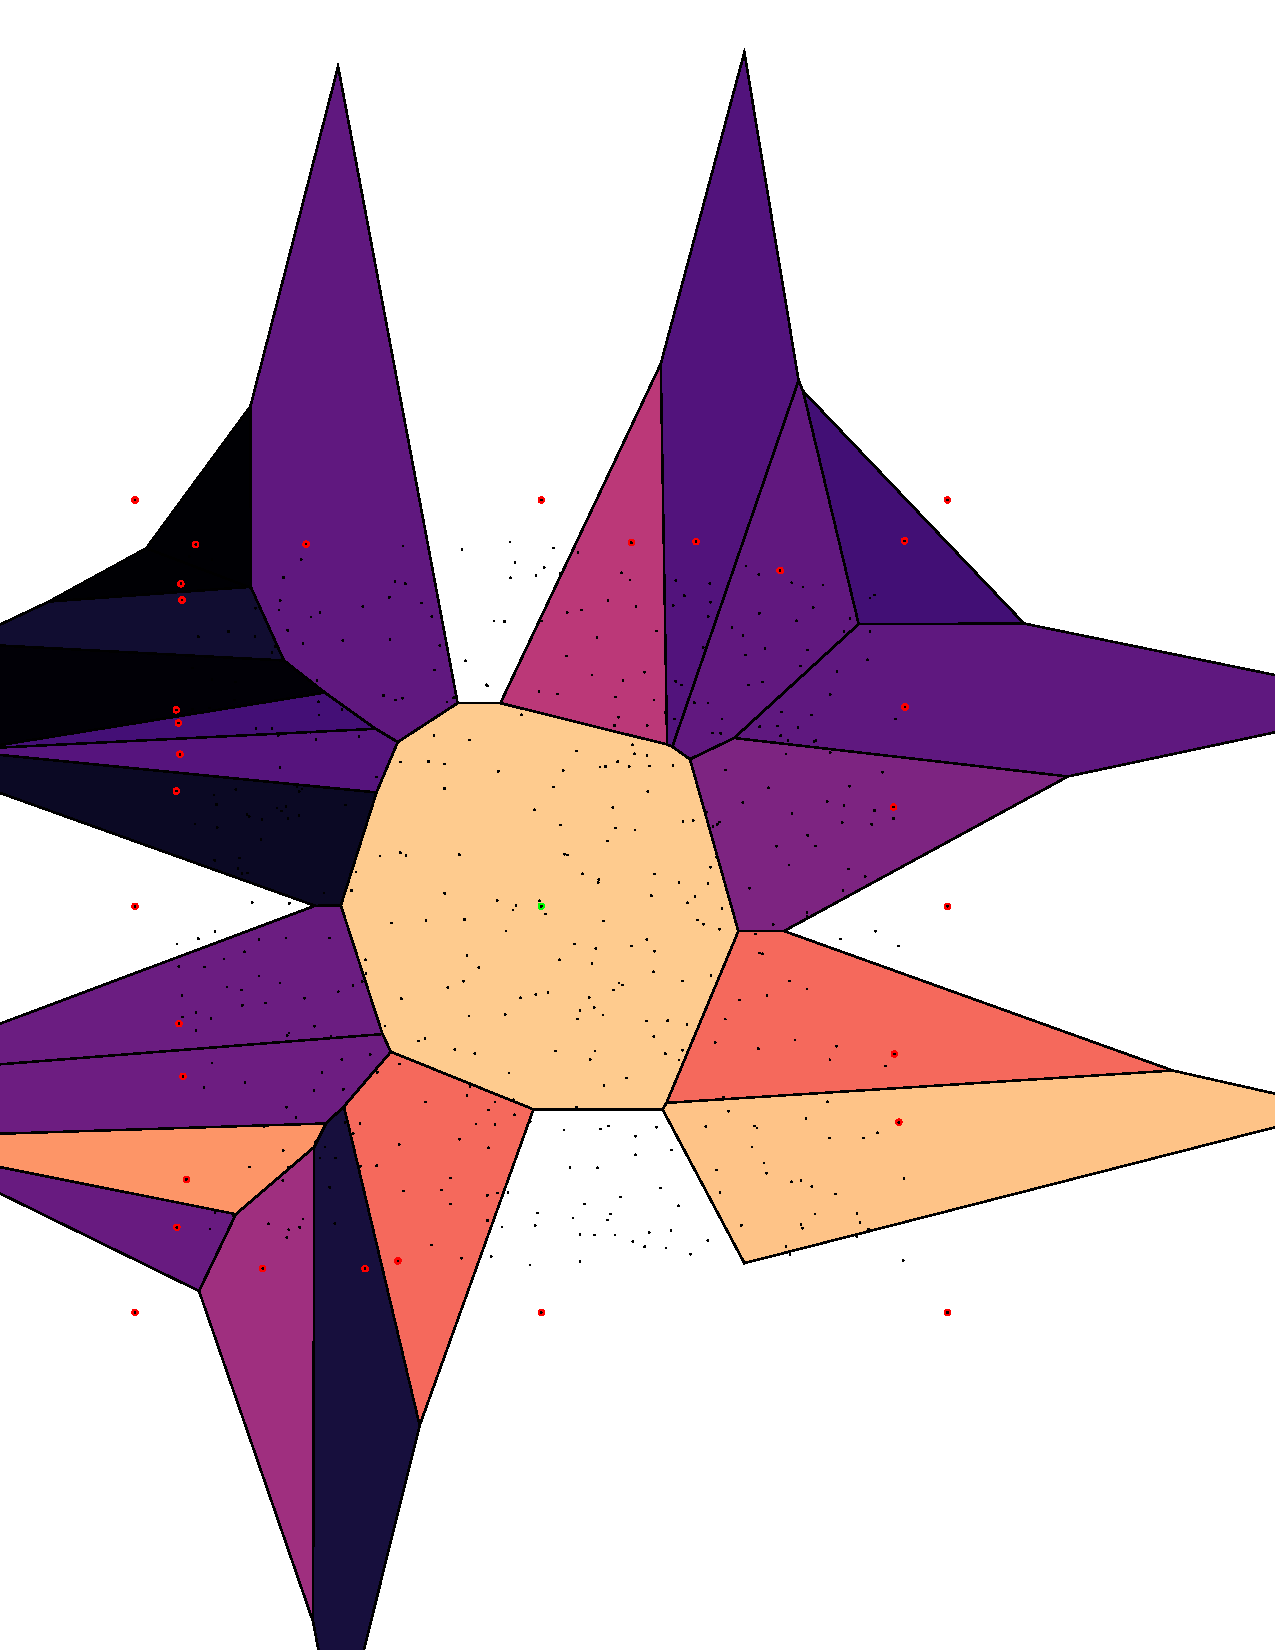
\includegraphics[trim={0 0 0 2cm},clip, width=0.2\textwidth]{../viz/500/voro_err0.pdf}}
   \subfloat [B] {\includegraphics[trim={0 0 0 2cm},clip, width=0.2\textwidth]{../viz/500/voro_err100.pdf}}
   \subfloat [C] {\includegraphics[trim={0 0 0 2cm},clip, width=0.2\textwidth]{../viz/500/voro_err200.pdf}}   
   \subfloat [D] {\includegraphics[trim={0 0 0 2cm},clip, width=0.2\textwidth]{../viz/500/voro_err300.pdf}}   
   \subfloat [E] {\includegraphics[trim={0 0 0 2cm},clip, width=0.2\textwidth]{../viz/500/voro_err400.pdf}}   

   

\end{figure}
%======================================================

\end{document}